%&preformat-disser
\RequirePackage[l2tabu,orthodox]{nag} % Раскомментировав, можно в логе получать рекомендации относительно правильного использования пакетов и предупреждения об устаревших и нерекомендуемых пакетах
% Формат А4, 14pt (ГОСТ Р 7.0.11-2011, 5.3.6)
\documentclass[a4paper,14pt,oneside,openany]{memoir}

%%%%%%%%%%%%%%%%%%%%%%%%%%%%%%%%%%%%%%%%%%%%%%%%%%%%%%%%%%%%%%%%%%%%%%%%%%%%%%%%
%%%% Файл упрощённых настроек шаблона, общих для диссертации и автореферата %%%%
%%%%%%%%%%%%%%%%%%%%%%%%%%%%%%%%%%%%%%%%%%%%%%%%%%%%%%%%%%%%%%%%%%%%%%%%%%%%%%%%

%%% Режим черновика %%%
\makeatletter
\@ifundefined{c@draft}{
  \newcounter{draft}
  \setcounter{draft}{0}  % 0 --- чистовик (максимальное соблюдение ГОСТ)
                         % 1 --- черновик (отклонения от ГОСТ, но быстрая
                         %       сборка итоговых PDF)
}{}
\makeatother

%%% Пометки в тексте %%%
\makeatletter
\@ifundefined{c@showmarkup}{
  \newcounter{showmarkup}
  \setcounter{showmarkup}{0}  % 0 --- скрыть пометки
                              % 1 --- показывать пометки
}{}
\makeatother

%%% Использование в pdflatex шрифтов не по-умолчанию %%%
\makeatletter
\@ifundefined{c@usealtfont}{
  \newcounter{usealtfont}
  \setcounter{usealtfont}{1}    % 0 --- шрифты на базе Computer Modern
                                % 1 --- использовать пакет pscyr, при его
                                %       наличии
                                % 2 --- использовать пакет XCharter, при наличии
                                %       подходящей версии
}{}
\makeatother

%%% Использование в xelatex и lualatex семейств шрифтов %%%
\makeatletter
\@ifundefined{c@fontfamily}{
  \newcounter{fontfamily}
  \setcounter{fontfamily}{1}  % 0 --- CMU семейство. Используется как fallback;
                              % 1 --- Шрифты от MS (Times New Roman и компания)
                              % 2 --- Семейство Liberation
}{}
\makeatother

%%% Библиография %%%
\makeatletter
\@ifundefined{c@bibliosel}{
  \newcounter{bibliosel}
  \setcounter{bibliosel}{1}   % 0 --- встроенная реализация с загрузкой файла
                              %       через движок bibtex8;
                              % 1 --- реализация пакетом biblatex через движок
                              %       biber
}{}
\makeatother

%%% Предкомпиляция tikz рисунков для ускорения работы %%%
\makeatletter
\@ifundefined{c@imgprecompile}{
  \newcounter{imgprecompile}
  \setcounter{imgprecompile}{0}   % 0 --- без предкомпиляции;
                                  % 1 --- пользоваться предварительно
                                  %       скомпилированными pdf вместо генерации
                                  %       заново из tikz
}{}
\makeatother
            % общие настройки шаблона
%%% Проверка используемого TeX-движка %%%
\newif\ifxetexorluatex   % определяем новый условный оператор (http://tex.stackexchange.com/a/47579)
\ifxetex
    \xetexorluatextrue
\else
    \ifluatex
        \xetexorluatextrue
    \else
        \xetexorluatexfalse
    \fi
\fi

\newif\ifsynopsis           % Условие, проверяющее, что документ --- автореферат

\usepackage{etoolbox}[2015/08/02]   % Для продвинутой проверки разных условий
\providebool{presentation}

\usepackage{comment}    % Позволяет убирать блоки текста (добавляет
                        % окружение comment и команду \excludecomment)

%%% Поля и разметка страницы %%%
\usepackage{pdflscape}  % Для включения альбомных страниц
\usepackage{geometry}   % Для последующего задания полей

%%% Математические пакеты %%%
\usepackage{amsthm,amsmath,amscd}   % Математические дополнения от AMS
\usepackage{amsfonts,amssymb}       % Математические дополнения от AMS
\usepackage{mathtools}              % Добавляет окружение multlined
\usepackage{xfrac}                  % Красивые дроби
\usepackage[
    locale = DE,
    list-separator       = {;\,},
    list-final-separator = {;\,},
    list-pair-separator  = {;\,},
    list-units           = single,
    range-units          = single,
    range-phrase={\text{\ensuremath{-}}},
    % quotient-mode        = fraction, % красивые дроби могут не соответствовать ГОСТ
    fraction-function    = \sfrac,
    separate-uncertainty,
    ]{siunitx}                      % Размерности SI
\sisetup{inter-unit-product = \ensuremath{{}\cdot{}}}

% Кириллица в нумерации subequations
% Для правильной работы требуется выполнение сразу после загрузки пакетов
\patchcmd{\subequations}{\def\theequation{\theparentequation\alph{equation}}}
{\def\theequation{\theparentequation\asbuk{equation}}}
{\typeout{subequations patched}}{\typeout{subequations not patched}}

%%%% Установки для размера шрифта 14 pt %%%%
%% Формирование переменных и констант для сравнения (один раз для всех подключаемых файлов)%%
%% должно располагаться до вызова пакета fontspec или polyglossia, потому что они сбивают его работу
\newlength{\curtextsize}
\newlength{\bigtextsize}
\setlength{\bigtextsize}{13.9pt}

\makeatletter
%\show\f@size    % неплохо для отслеживания, но вызывает стопорение процесса,
                 % если документ компилируется без команды  -interaction=nonstopmode
\setlength{\curtextsize}{\f@size pt}
\makeatother

%%% Кодировки и шрифты %%%
\ifxetexorluatex
    \PassOptionsToPackage{no-math}{fontspec}    % https://tex.stackexchange.com/a/26295/104425
    \usepackage{polyglossia}[2014/05/21]        % Поддержка многоязычности
                                        % (fontspec подгружается автоматически)
\else
   %%% Решение проблемы копирования текста в буфер кракозябрами
    \ifnumequal{\value{usealtfont}}{0}{}{
        \input glyphtounicode.tex
        \input glyphtounicode-cmr.tex %from pdfx package
        \pdfgentounicode=1
    }
    \usepackage{cmap}   % Улучшенный поиск русских слов в полученном pdf-файле
    \ifnumequal{\value{usealtfont}}{2}{}{
        \defaulthyphenchar=127  % Если стоит до fontenc, то переносы
                                % не впишутся в выделяемый текст при
                                % копировании его в буфер обмена
    }
    \usepackage{textcomp}
    \usepackage[T1,T2A]{fontenc}                    % Поддержка русских букв
    \ifnumequal{\value{usealtfont}}{1}{% Используется pscyr, при наличии
        \IfFileExists{pscyr.sty}{\usepackage{pscyr}}{}  % Подключение pscyr
    }{}
    \usepackage[utf8]{inputenc}[2014/04/30]         % Кодировка utf8
    \usepackage[english, russian]{babel}[2014/03/24]% Языки: русский, английский
    \makeatletter\AtBeginDocument{\let\@elt\relax}\makeatother % babel 3.40 fix
    \ifnumequal{\value{usealtfont}}{2}{
        % http://dxdy.ru/post1238763.html#p1238763
        \usepackage[scaled=0.960]{XCharter}[2017/12/19] % Подключение русифицированных шрифтов XCharter
        \usepackage[charter, vvarbb, scaled=1.048]{newtxmath}[2017/12/14]
        \ifpresentation
        \else
            \setDisplayskipStretch{-0.078}
        \fi
    }{}
\fi

%%% Оформление абзацев %%%
\ifpresentation
\else
    \indentafterchapter     % Красная строка после заголовков типа chapter
\fi

%%% Цвета %%%
\ifpresentation
\else
    \usepackage[dvipsnames, table, hyperref]{xcolor} % Совместимо с tikz
\fi

%%% Таблицы %%%
\usepackage{longtable,ltcaption} % Длинные таблицы
\usepackage{multirow,makecell}   % Улучшенное форматирование таблиц
\usepackage{tabu, tabulary}      % таблицы с автоматически подбирающейся
                                 % шириной столбцов (tabu обязательно
                                 % до hyperref вызывать)
\usepackage{threeparttable}      % автоматический подгон ширины подписи таблицы

%%% Общее форматирование
\usepackage{soulutf8}% Поддержка переносоустойчивых подчёркиваний и зачёркиваний
\usepackage{icomma}  % Запятая в десятичных дробях

%%% Оптимизация расстановки переносов и длины последней строки абзаца
\IfFileExists{impnattypo.sty}{% проверка установленности пакета impnattypo
    \ifluatex
        \ifnumequal{\value{draft}}{1}{% Черновик
            \usepackage[hyphenation, lastparline, nosingleletter, homeoarchy,
            rivers, draft]{impnattypo}
        }{% Чистовик
            \usepackage[hyphenation, lastparline, nosingleletter]{impnattypo}
        }
    \else
        \usepackage[hyphenation, lastparline]{impnattypo}
    \fi
}{}

%% Векторная графика

\usepackage{tikz}                   % Продвинутый пакет векторной графики
\usetikzlibrary{chains}             % Для примера tikz рисунка
\usetikzlibrary{shapes.geometric}   % Для примера tikz рисунка
\usetikzlibrary{shapes.symbols}     % Для примера tikz рисунка
\usetikzlibrary{arrows}             % Для примера tikz рисунка

%%% Гиперссылки %%%
\usepackage{hyperref}[2012/11/06]

%%% Изображения %%%
\usepackage{graphicx}[2014/04/25]   % Подключаем пакет работы с графикой
\usepackage{caption}                % Подписи рисунков и таблиц
\usepackage{subcaption}             % Подписи подрисунков и подтаблиц
\usepackage{pdfpages}               % Добавление внешних pdf файлов

%%% Счётчики %%%
\usepackage[figure,table]{totalcount}   % Счётчик рисунков и таблиц
\usepackage{totcount}   % Пакет создания счётчиков на основе последнего номера
                        % подсчитываемого элемента (может требовать дважды
                        % компилировать документ)
\usepackage{totpages}   % Счётчик страниц, совместимый с hyperref (ссылается
                        % на номер последней страницы). Желательно ставить
                        % последним пакетом в преамбуле

%%% Продвинутое управление групповыми ссылками (пока только формулами) %%%
\ifpresentation
\else
    \usepackage[russian]{cleveref} % cleveref имеет сложности со считыванием
    % языка из babel. Такое решение русификации вывода выбрано вместо
    % определения в documentclass из опасности что-то лишнее передать во все
    % остальные пакеты, включая библиографию.
    \creflabelformat{equation}{#2#1#3} % Формат по умолчанию ставил круглые
    % скобки вокруг каждого номера ссылки, теперь просто номера ссылок без
    % какого-либо дополнительного оформления
    \crefrangelabelformat{equation}{#3#1#4\cyrdash#5#2#6} % Интервалы в русском
    % языке принято делать через тире, если иное не оговорено

    % решение проблемы с "и" в \labelcref
    % https://tex.stackexchange.com/a/455124/104425
    \ifxetexorluatex
        \DeclareTextSymbol{\cyri}\UnicodeEncodingName{"0438} % и
    \fi

    % Добавление возможности использования пробелов в \labelcref
    % https://tex.stackexchange.com/a/340502/104425
    \usepackage{kvsetkeys}
    \makeatletter
    \let\org@@cref\@cref
    \renewcommand*{\@cref}[2]{%
        \edef\process@me{%
            \noexpand\org@@cref{#1}{\zap@space#2 \@empty}%
        }\process@me
    }
    \makeatother

    \newcommand{\eqrefs}[1]{(\labelcref{#1})}
    \newcommand{\refs}[1]{\labelcref{#1}}
\fi

\usepackage{placeins} % для \FloatBarrier

\ifnumequal{\value{draft}}{1}{% Черновик
    \usepackage[firstpage]{draftwatermark}
    \SetWatermarkText{DRAFT}
    \SetWatermarkFontSize{14pt}
    \SetWatermarkScale{15}
    \SetWatermarkAngle{45}
}{}

%%% Цитата, не приводимая в автореферате:
% возможно, актуальна только для biblatex
%\newcommand{\citeinsynopsis}[1]{\ifsynopsis\else ~\cite{#1} \fi}

% если текущий процесс запущен библиотекой tikz-external, то прекомпиляция должна быть включена
\ifdefined\tikzexternalrealjob
    \setcounter{imgprecompile}{1}
\fi

\ifnumequal{\value{imgprecompile}}{1}{% Только если у нас включена предкомпиляция
    \usetikzlibrary{external}   % подключение возможности предкомпиляции
    \tikzexternalize[prefix=images/cache/,optimize command away=\includepdf] % activate! % здесь можно указать отдельную папку для скомпилированных файлов
    \ifxetex
        \tikzset{external/up to date check={diff}}
    \fi
}{}
         % Пакеты общие для диссертации и автореферата
\synopsisfalse                      % Этот документ --- не автореферат
\input{Dissertation/dispackages}    % Пакеты для диссертации
\input{Dissertation/userpackages}   % Пакеты для специфических пользовательских задач

%%%%%%%%%%%%%%%%%%%%%%%%%%%%%%%%%%%%%%%%%%%%%%%%%%%%%%%%%%%%%%%%%%%%%%%%%%%%%%%%
%%%% Файл упрощённых настроек шаблона, общих для диссертации и автореферата %%%%
%%%%%%%%%%%%%%%%%%%%%%%%%%%%%%%%%%%%%%%%%%%%%%%%%%%%%%%%%%%%%%%%%%%%%%%%%%%%%%%%

%%% Режим черновика %%%
\makeatletter
\@ifundefined{c@draft}{
  \newcounter{draft}
  \setcounter{draft}{0}  % 0 --- чистовик (максимальное соблюдение ГОСТ)
                         % 1 --- черновик (отклонения от ГОСТ, но быстрая
                         %       сборка итоговых PDF)
}{}
\makeatother

%%% Пометки в тексте %%%
\makeatletter
\@ifundefined{c@showmarkup}{
  \newcounter{showmarkup}
  \setcounter{showmarkup}{0}  % 0 --- скрыть пометки
                              % 1 --- показывать пометки
}{}
\makeatother

%%% Использование в pdflatex шрифтов не по-умолчанию %%%
\makeatletter
\@ifundefined{c@usealtfont}{
  \newcounter{usealtfont}
  \setcounter{usealtfont}{1}    % 0 --- шрифты на базе Computer Modern
                                % 1 --- использовать пакет pscyr, при его
                                %       наличии
                                % 2 --- использовать пакет XCharter, при наличии
                                %       подходящей версии
}{}
\makeatother

%%% Использование в xelatex и lualatex семейств шрифтов %%%
\makeatletter
\@ifundefined{c@fontfamily}{
  \newcounter{fontfamily}
  \setcounter{fontfamily}{1}  % 0 --- CMU семейство. Используется как fallback;
                              % 1 --- Шрифты от MS (Times New Roman и компания)
                              % 2 --- Семейство Liberation
}{}
\makeatother

%%% Библиография %%%
\makeatletter
\@ifundefined{c@bibliosel}{
  \newcounter{bibliosel}
  \setcounter{bibliosel}{1}   % 0 --- встроенная реализация с загрузкой файла
                              %       через движок bibtex8;
                              % 1 --- реализация пакетом biblatex через движок
                              %       biber
}{}
\makeatother

%%% Предкомпиляция tikz рисунков для ускорения работы %%%
\makeatletter
\@ifundefined{c@imgprecompile}{
  \newcounter{imgprecompile}
  \setcounter{imgprecompile}{0}   % 0 --- без предкомпиляции;
                                  % 1 --- пользоваться предварительно
                                  %       скомпилированными pdf вместо генерации
                                  %       заново из tikz
}{}
\makeatother
      % Упрощённые настройки шаблона

% Новые переменные, которые могут использоваться во всём проекте
% ГОСТ 7.0.11-2011
% 9.2 Оформление текста автореферата диссертации
% 9.2.1 Общая характеристика работы включает в себя следующие основные структурные
% элементы:
% актуальность темы исследования;
\newcommand{\actualityTXT}{Актуальность темы.}
% степень ее разработанности;
\newcommand{\progressTXT}{Степень разработанности темы.}
% цели и задачи;
\newcommand{\aimTXT}{Целью}
\newcommand{\tasksTXT}{задачи}
% научную новизну;
\newcommand{\noveltyTXT}{Научная новизна:}
% теоретическую и практическую значимость работы;
%\newcommand{\influenceTXT}{Теоретическая и практическая значимость}
% или чаще используют просто
\newcommand{\influenceTXT}{Практическая значимость}
% методологию и методы исследования;
\newcommand{\methodsTXT}{Методология и методы исследования.}
% положения, выносимые на защиту;
\newcommand{\defpositionsTXT}{Основные положения, выносимые на~защиту:}
% степень достоверности и апробацию результатов.
\newcommand{\reliabilityTXT}{Достоверность}
\newcommand{\probationTXT}{Апробация работы.}

\newcommand{\contributionTXT}{Личный вклад.}
\newcommand{\publicationsTXT}{Публикации.}


%%% Заголовки библиографии:

% для автореферата:
\newcommand{\bibtitleauthor}{Публикации автора по теме диссертации}

% для стиля библиографии `\insertbiblioauthorgrouped`
\newcommand{\bibtitleauthorvak}{В изданиях из списка ВАК РФ}
\newcommand{\bibtitleauthorscopus}{В изданиях, входящих в международную базу цитирования Scopus}
\newcommand{\bibtitleauthorwos}{В изданиях, входящих в международную базу цитирования Web of Science}
\newcommand{\bibtitleauthorother}{В прочих изданиях}
\newcommand{\bibtitleauthorconf}{В сборниках трудов конференций}

% для стиля библиографии `\insertbiblioauthorimportant`:
\newcommand{\bibtitleauthorimportant}{Наиболее значимые \protect\MakeLowercase\bibtitleauthor}

% для списка литературы в диссертации и списка чужих работ в автореферате:
\newcommand{\bibtitlefull}{Список литературы} % (ГОСТ Р 7.0.11-2011, 4)
         % Новые переменные, для всего проекта

%%% Основные сведения %%%
\newcommand{\thesisAuthorLastName}{Чепрасов}
\newcommand{\thesisAuthorOtherNames}{Иван Андреевич}
\newcommand{\thesisAuthorInitials}{И.\,А.}
\newcommand{\thesisAuthor}             % Диссертация, ФИО автора
{%
    \texorpdfstring{% \texorpdfstring takes two arguments and uses the first for (La)TeX and the second for pdf
        \thesisAuthorLastName~\thesisAuthorOtherNames% так будет отображаться на титульном листе или в тексте, где будет использоваться переменная
    }{%
        \thesisAuthorLastName, \thesisAuthorOtherNames% эта запись для свойств pdf-файла. В таком виде, если pdf будет обработан программами для сбора библиографических сведений, будет правильно представлена фамилия.
    }
}
\newcommand{\thesisAuthorShort}        % Диссертация, ФИО автора инициалами
{\thesisAuthorInitials~\thesisAuthorLastName}
%\newcommand{\thesisUdk}                % Диссертация, УДК
%{\fixme{xxx.xxx}}
\newcommand{\thesisTitle}              % Диссертация, название
{{Термодинамически согласованная модель фильтрации в упругой хрупкой среде с двойной пористостью}}
\newcommand{\thesisSpecialtyNumber}    % Диссертация, специальность, номер
{03.04.01}
\newcommand{\thesisSpecialtyTitle}     % Диссертация, специальность, название (название взято с сайта ВАК для примера)
{{Прикладные математика и физика}}
%% \newcommand{\thesisSpecialtyTwoNumber} % Диссертация, вторая специальность, номер
%% {\fixme{XX.XX.XX}}
%% \newcommand{\thesisSpecialtyTwoTitle}  % Диссертация, вторая специальность, название
%% {\fixme{Теория и~методика физического воспитания, спортивной тренировки,
%% оздоровительной и~адаптивной физической культуры}}
\newcommand{\thesisDegree}             % Диссертация, ученая степень
{{магистра}}
\newcommand{\thesisDegreeShort}        % Диссертация, ученая степень, краткая запись
{\fixme{канд. физ.-мат. наук}}
\newcommand{\thesisCity}               % Диссертация, город написания диссертации
{{Долгопрудный}}
\newcommand{\thesisYear}               % Диссертация, год написания диссертации
{\the\year}
\newcommand{\thesisOrganization}       % Диссертация, организация
{{Федеральное государственное автономное образовательное учреждение высшего образования <<Московский физико-технический институт (национальный исследовательский университет)>>
\\
<<МФТИ>>}}
\newcommand{\thesisOrganizationShort}  % Диссертация, краткое название организации для доклада
{\fixme{МФТИ}}

\newcommand{\thesisInOrganization}     % Диссертация, организация в предложном падеже: Работа выполнена в ...
{Московском физико-техническом институте (НИУ)}

%% \newcommand{\supervisorDead}{}           % Рисовать рамку вокруг фамилии
\newcommand{\supervisorFio}              % Научный руководитель, ФИО
{{Извеков Олег Ярославович}}
\newcommand{\supervisorRegalia}          % Научный руководитель, регалии
{{кандидат физико-математических наук}}
\newcommand{\supervisorFioShort}         % Научный руководитель, ФИО
{{О.\,Я.~Извеков}}
\newcommand{\supervisorRegaliaShort}     % Научный руководитель, регалии
{{к.ф.-м.н.}}

%% \newcommand{\supervisorTwoDead}{}        % Рисовать рамку вокруг фамилии
%% \newcommand{\supervisorTwoFio}           % Второй научный руководитель, ФИО
%% {\fixme{Фамилия Имя Отчество}}
%% \newcommand{\supervisorTwoRegalia}       % Второй научный руководитель, регалии
%% {\fixme{уч. степень, уч. звание}}
%% \newcommand{\supervisorTwoFioShort}      % Второй научный руководитель, ФИО
%% {\fixme{И.\,О.~Фамилия}}
%% \newcommand{\supervisorTwoRegaliaShort}  % Второй научный руководитель, регалии
%% {\fixme{уч.~ст.,~уч.~зв.}}

\newcommand{\opponentOneFio}           % Оппонент 1, ФИО
{\fixme{Фамилия Имя Отчество}}
\newcommand{\opponentOneRegalia}       % Оппонент 1, регалии
{\fixme{доктор физико-математических наук, профессор}}
\newcommand{\opponentOneJobPlace}      % Оппонент 1, место работы
{\fixme{Не очень длинное название для места работы}}
\newcommand{\opponentOneJobPost}       % Оппонент 1, должность
{\fixme{старший научный сотрудник}}

\newcommand{\opponentTwoFio}           % Оппонент 2, ФИО
{\fixme{Фамилия Имя Отчество}}
\newcommand{\opponentTwoRegalia}       % Оппонент 2, регалии
{\fixme{кандидат физико-математических наук}}
\newcommand{\opponentTwoJobPlace}      % Оппонент 2, место работы
{\fixme{Основное место работы c длинным длинным длинным длинным названием}}
\newcommand{\opponentTwoJobPost}       % Оппонент 2, должность
{\fixme{старший научный сотрудник}}

%% \newcommand{\opponentThreeFio}         % Оппонент 3, ФИО
%% {\fixme{Фамилия Имя Отчество}}
%% \newcommand{\opponentThreeRegalia}     % Оппонент 3, регалии
%% {\fixme{кандидат физико-математических наук}}
%% \newcommand{\opponentThreeJobPlace}    % Оппонент 3, место работы
%% {\fixme{Основное место работы c длинным длинным длинным длинным названием}}
%% \newcommand{\opponentThreeJobPost}     % Оппонент 3, должность
%% {\fixme{старший научный сотрудник}}

\newcommand{\leadingOrganizationTitle} % Ведущая организация, дополнительные строки. Удалить, чтобы не отображать в автореферате
{\fixme{Федеральное государственное бюджетное образовательное учреждение высшего
профессионального образования с~длинным длинным длинным длинным названием}}

\newcommand{\defenseDate}              % Защита, дата
{\fixme{DD mmmmmmmm YYYY~г.~в~XX часов}}
\newcommand{\defenseCouncilNumber}     % Защита, номер диссертационного совета
{\fixme{Д\,123.456.78}}
\newcommand{\defenseCouncilTitle}      % Защита, учреждение диссертационного совета
{\fixme{Название учреждения}}
\newcommand{\defenseCouncilAddress}    % Защита, адрес учреждение диссертационного совета
{\fixme{Адрес}}
\newcommand{\defenseCouncilPhone}      % Телефон для справок
{\fixme{+7~(0000)~00-00-00}}

\newcommand{\defenseSecretaryFio}      % Секретарь диссертационного совета, ФИО
{\fixme{Фамилия Имя Отчество}}
\newcommand{\defenseSecretaryRegalia}  % Секретарь диссертационного совета, регалии
{\fixme{д-р~физ.-мат. наук}}            % Для сокращений есть ГОСТы, например: ГОСТ Р 7.0.12-2011 + http://base.garant.ru/179724/#block_30000

\newcommand{\synopsisLibrary}          % Автореферат, название библиотеки
{\fixme{Название библиотеки}}
\newcommand{\synopsisDate}             % Автореферат, дата рассылки
{\fixme{DD mmmmmmmm}\the\year~года}

% To avoid conflict with beamer class use \providecommand
\providecommand{\keywords}%            % Ключевые слова для метаданных PDF диссертации и автореферата
{}
             % Основные сведения
%%% Кодировки и шрифты %%%
\ifxetexorluatex
    \setmainlanguage[babelshorthands=true]{russian}    % Язык по-умолчанию русский с поддержкой приятных команд пакета babel
    \setotherlanguage{english}                         % Дополнительный язык = английский (в американской вариации по-умолчанию)

    % Проверка существования шрифтов. Недоступна в pdflatex
    \ifnumequal{\value{fontfamily}}{1}{
        \IfFontExistsTF{Times New Roman}{}{\setcounter{fontfamily}{0}}
    }{}
    \ifnumequal{\value{fontfamily}}{2}{
        \IfFontExistsTF{LiberationSerif}{}{\setcounter{fontfamily}{0}}
    }{}

    \ifnumequal{\value{fontfamily}}{0}{                    % Семейство шрифтов CMU. Используется как fallback
        \setmonofont{CMU Typewriter Text}                  % моноширинный шрифт
        \newfontfamily\cyrillicfonttt{CMU Typewriter Text} % моноширинный шрифт для кириллицы
        \defaultfontfeatures{Ligatures=TeX}                % стандартные лигатуры TeX, замены нескольких дефисов на тире и т. п. Настройки моноширинного шрифта должны идти до этой строки, чтобы при врезках кода программ в коде не применялись лигатуры и замены дефисов
        \setmainfont{CMU Serif}                            % Шрифт с засечками
        \newfontfamily\cyrillicfont{CMU Serif}             % Шрифт с засечками для кириллицы
        \setsansfont{CMU Sans Serif}                       % Шрифт без засечек
        \newfontfamily\cyrillicfontsf{CMU Sans Serif}      % Шрифт без засечек для кириллицы
    }

    \ifnumequal{\value{fontfamily}}{1}{                    % Семейство MS шрифтов
        \setmonofont{Courier New}                          % моноширинный шрифт
        \newfontfamily\cyrillicfonttt{Courier New}         % моноширинный шрифт для кириллицы
        \defaultfontfeatures{Ligatures=TeX}                % стандартные лигатуры TeX, замены нескольких дефисов на тире и т. п. Настройки моноширинного шрифта должны идти до этой строки, чтобы при врезках кода программ в коде не применялись лигатуры и замены дефисов
        \setmainfont{Times New Roman}                      % Шрифт с засечками
        \newfontfamily\cyrillicfont{Times New Roman}       % Шрифт с засечками для кириллицы
        \setsansfont{Arial}                                % Шрифт без засечек
        \newfontfamily\cyrillicfontsf{Arial}               % Шрифт без засечек для кириллицы
    }

    \ifnumequal{\value{fontfamily}}{2}{                    % Семейство шрифтов Liberation (https://pagure.io/liberation-fonts)
        \setmonofont{LiberationMono}[Scale=0.87] % моноширинный шрифт
        \newfontfamily\cyrillicfonttt{LiberationMono}[     % моноширинный шрифт для кириллицы
            Scale=0.87]
        \defaultfontfeatures{Ligatures=TeX}                % стандартные лигатуры TeX, замены нескольких дефисов на тире и т. п. Настройки моноширинного шрифта должны идти до этой строки, чтобы при врезках кода программ в коде не применялись лигатуры и замены дефисов
        \setmainfont{LiberationSerif}                      % Шрифт с засечками
        \newfontfamily\cyrillicfont{LiberationSerif}       % Шрифт с засечками для кириллицы
        \setsansfont{LiberationSans}                       % Шрифт без засечек
        \newfontfamily\cyrillicfontsf{LiberationSans}      % Шрифт без засечек для кириллицы
    }

\else
    \ifnumequal{\value{usealtfont}}{1}{% Используется pscyr, при наличии
        \IfFileExists{pscyr.sty}{\renewcommand{\rmdefault}{ftm}}{}
    }{}
\fi
            % Определение шрифтов (частичное)
%%% Шаблон %%%
\DeclareRobustCommand{\fixme}{\textcolor{red}}  % решаем проблему превращения
                                % названия цвета в результате \MakeUppercase,
                                % http://tex.stackexchange.com/a/187930,
                                % \DeclareRobustCommand protects \fixme
                                % from expanding inside \MakeUppercase
\AtBeginDocument{%
    \setlength{\parindent}{2.5em}                   % Абзацный отступ. Должен быть одинаковым по всему тексту и равен пяти знакам (ГОСТ Р 7.0.11-2011, 5.3.7).
}

%%% Таблицы %%%
\DeclareCaptionLabelSeparator{tabsep}{\tablabelsep} % нумерация таблиц
\DeclareCaptionFormat{split}{\splitformatlabel#1\par\splitformattext#3}

\captionsetup[table]{
        format=\tabformat,                % формат подписи (plain|hang)
        font=normal,                      % нормальные размер, цвет, стиль шрифта
        skip=.0pt,                        % отбивка под подписью
        parskip=.0pt,                     % отбивка между параграфами подписи
        position=above,                   % положение подписи
        justification=\tabjust,           % центровка
        indent=\tabindent,                % смещение строк после первой
        labelsep=tabsep,                  % разделитель
        singlelinecheck=\tabsinglecenter, % не выравнивать по центру, если умещается в одну строку
}

%%% Рисунки %%%
\DeclareCaptionLabelSeparator{figsep}{\figlabelsep} % нумерация рисунков

\captionsetup[figure]{
        format=plain,                     % формат подписи (plain|hang)
        font=normal,                      % нормальные размер, цвет, стиль шрифта
        skip=.0pt,                        % отбивка под подписью
        parskip=.0pt,                     % отбивка между параграфами подписи
        position=below,                   % положение подписи
        singlelinecheck=true,             % выравнивание по центру, если умещается в одну строку
        justification=centerlast,         % центровка
        labelsep=figsep,                  % разделитель
}

%%% Подписи подрисунков %%%
\DeclareCaptionSubType{figure}
\renewcommand\thesubfigure{\asbuk{subfigure}} % нумерация подрисунков
\ifsynopsis
\DeclareCaptionFont{norm}{\fontsize{10pt}{11pt}\selectfont}
\newcommand{\subfigureskip}{2.pt}
\else
\DeclareCaptionFont{norm}{\fontsize{14pt}{16pt}\selectfont}
\newcommand{\subfigureskip}{0.pt}
\fi

\captionsetup[subfloat]{
        labelfont=norm,                 % нормальный размер подписей подрисунков
        textfont=norm,                  % нормальный размер подписей подрисунков
        labelsep=space,                 % разделитель
        labelformat=brace,              % одна скобка справа от номера
        justification=centering,        % центровка
        singlelinecheck=true,           % выравнивание по центру, если умещается в одну строку
        skip=\subfigureskip,            % отбивка над подписью
        parskip=.0pt,                   % отбивка между параграфами подписи
        position=below,                 % положение подписи
}

%%% Настройки гиперссылок %%%
\ifluatex
    \hypersetup{
        unicode,                % Unicode encoded PDF strings
    }
\fi

\hypersetup{
    linktocpage=true,           % ссылки с номера страницы в оглавлении, списке таблиц и списке рисунков
%    linktoc=all,                % both the section and page part are links
%    pdfpagelabels=false,        % set PDF page labels (true|false)
    plainpages=false,           % Forces page anchors to be named by the Arabic form  of the page number, rather than the formatted form
    colorlinks,                 % ссылки отображаются раскрашенным текстом, а не раскрашенным прямоугольником, вокруг текста
    linkcolor={linkcolor},      % цвет ссылок типа ref, eqref и подобных
    citecolor={citecolor},      % цвет ссылок-цитат
    urlcolor={urlcolor},        % цвет гиперссылок
%    hidelinks,                  % Hide links (removing color and border)
    pdftitle={\thesisTitle},    % Заголовок
    pdfauthor={\thesisAuthor},  % Автор
    pdfsubject={\thesisSpecialtyNumber\ \thesisSpecialtyTitle},      % Тема
%    pdfcreator={Создатель},     % Создатель, Приложение
%    pdfproducer={Производитель},% Производитель, Производитель PDF
    pdfkeywords={\keywords},    % Ключевые слова
    pdflang={ru},
}
\ifnumequal{\value{draft}}{1}{% Черновик
    \hypersetup{
        draft,
    }
}{}

%%% Списки %%%
% Используем короткое тире (endash) для ненумерованных списков (ГОСТ 2.105-95, пункт 4.1.7, требует дефиса, но так лучше смотрится)
\renewcommand{\labelitemi}{\normalfont\bfseries{--}}

% Перечисление строчными буквами латинского алфавита (ГОСТ 2.105-95, 4.1.7)
%\renewcommand{\theenumi}{\alph{enumi}}
%\renewcommand{\labelenumi}{\theenumi)}

% Перечисление строчными буквами русского алфавита (ГОСТ 2.105-95, 4.1.7)
\makeatletter
\AddEnumerateCounter{\asbuk}{\russian@alph}{щ}      % Управляем списками/перечислениями через пакет enumitem, а он 'не знает' про asbuk, потому 'учим' его
\makeatother
%\renewcommand{\theenumi}{\asbuk{enumi}} %первый уровень нумерации
%\renewcommand{\labelenumi}{\theenumi)} %первый уровень нумерации
\renewcommand{\theenumii}{\asbuk{enumii}} %второй уровень нумерации
\renewcommand{\labelenumii}{\theenumii)} %второй уровень нумерации
\renewcommand{\theenumiii}{\arabic{enumiii}} %третий уровень нумерации
\renewcommand{\labelenumiii}{\theenumiii)} %третий уровень нумерации

\setlist{nosep,%                                    % Единый стиль для всех списков (пакет enumitem), без дополнительных интервалов.
    labelindent=\parindent,leftmargin=*%            % Каждый пункт, подпункт и перечисление записывают с абзацного отступа (ГОСТ 2.105-95, 4.1.8)
}

%%% Правильная нумерация приложений, рисунков и формул %%%
%% По ГОСТ 2.105, п. 4.3.8 Приложения обозначают заглавными буквами русского алфавита,
%% начиная с А, за исключением букв Ё, З, Й, О, Ч, Ь, Ы, Ъ.
%% Здесь также переделаны все нумерации русскими буквами.
\ifxetexorluatex
    \makeatletter
    \def\russian@Alph#1{\ifcase#1\or
       А\or Б\or В\or Г\or Д\or Е\or Ж\or
       И\or К\or Л\or М\or Н\or
       П\or Р\or С\or Т\or У\or Ф\or Х\or
       Ц\or Ш\or Щ\or Э\or Ю\or Я\else\xpg@ill@value{#1}{russian@Alph}\fi}
    \def\russian@alph#1{\ifcase#1\or
       а\or б\or в\or г\or д\or е\or ж\or
       и\or к\or л\or м\or н\or
       п\or р\or с\or т\or у\or ф\or х\or
       ц\or ш\or щ\or э\or ю\or я\else\xpg@ill@value{#1}{russian@alph}\fi}
    \def\cyr@Alph#1{\ifcase#1\or
        А\or Б\or В\or Г\or Д\or Е\or Ж\or
        И\or К\or Л\or М\or Н\or
        П\or Р\or С\or Т\or У\or Ф\or Х\or
        Ц\or Ш\or Щ\or Э\or Ю\or Я\else\xpg@ill@value{#1}{cyr@Alph}\fi}
    \def\cyr@alph#1{\ifcase#1\or
        а\or б\or в\or г\or д\or е\or ж\or
        и\or к\or л\or м\or н\or
        п\or р\or с\or т\or у\or ф\or х\or
        ц\or ш\or щ\or э\or ю\or я\else\xpg@ill@value{#1}{cyr@alph}\fi}
    \makeatother
\else
    \makeatletter
    \if@uni@ode
      \def\russian@Alph#1{\ifcase#1\or
        А\or Б\or В\or Г\or Д\or Е\or Ж\or
        И\or К\or Л\or М\or Н\or
        П\or Р\or С\or Т\or У\or Ф\or Х\or
        Ц\or Ш\or Щ\or Э\or Ю\or Я\else\@ctrerr\fi}
    \else
      \def\russian@Alph#1{\ifcase#1\or
        \CYRA\or\CYRB\or\CYRV\or\CYRG\or\CYRD\or\CYRE\or\CYRZH\or
        \CYRI\or\CYRK\or\CYRL\or\CYRM\or\CYRN\or
        \CYRP\or\CYRR\or\CYRS\or\CYRT\or\CYRU\or\CYRF\or\CYRH\or
        \CYRC\or\CYRSH\or\CYRSHCH\or\CYREREV\or\CYRYU\or
        \CYRYA\else\@ctrerr\fi}
    \fi
    \if@uni@ode
      \def\russian@alph#1{\ifcase#1\or
        а\or б\or в\or г\or д\or е\or ж\or
        и\or к\or л\or м\or н\or
        п\or р\or с\or т\or у\or ф\or х\or
        ц\or ш\or щ\or э\or ю\or я\else\@ctrerr\fi}
    \else
      \def\russian@alph#1{\ifcase#1\or
        \cyra\or\cyrb\or\cyrv\or\cyrg\or\cyrd\or\cyre\or\cyrzh\or
        \cyri\or\cyrk\or\cyrl\or\cyrm\or\cyrn\or
        \cyrp\or\cyrr\or\cyrs\or\cyrt\or\cyru\or\cyrf\or\cyrh\or
        \cyrc\or\cyrsh\or\cyrshch\or\cyrerev\or\cyryu\or
        \cyrya\else\@ctrerr\fi}
    \fi
    \makeatother
\fi

%%% Команды рецензирования %%%
\ifboolexpr{ (test {\ifnumequal{\value{draft}}{1}}) or (test {\ifnumequal{\value{showmarkup}}{1}})}{
        \newrobustcmd{\todo}[1]{\textcolor{red}{#1}}
        \newrobustcmd{\note}[2][]{\ifstrempty{#1}{#2}{\textcolor{#1}{#2}}}
        \newenvironment{commentbox}[1][]%
        {\ifstrempty{#1}{}{\color{#1}}}%
        {}
}{
        \newrobustcmd{\todo}[1]{}
        \newrobustcmd{\note}[2][]{}
        \excludecomment{commentbox}
}

           % Стили общие для диссертации и автореферата
%%% Переопределение именований, если иначе не сработает %%%
%\gappto\captionsrussian{
%    \renewcommand{\chaptername}{Глава}
%    \renewcommand{\appendixname}{Приложение} % (ГОСТ Р 7.0.11-2011, 5.7)
%}

%%% Изображения %%%
\graphicspath{{images/}{Dissertation/images/}}         % Пути к изображениям

%%% Интервалы %%%
%% По ГОСТ Р 7.0.11-2011, пункту 5.3.6 требуется полуторный интервал
%% Реализация средствами класса (на основе setspace) ближе к типографской классике.
%% И правит сразу и в таблицах (если со звёздочкой)
%\DoubleSpacing*     % Двойной интервал
\OnehalfSpacing*    % Полуторный интервал
%\setSpacing{1.42}   % Полуторный интервал, подобный Ворду (возможно, стоит включать вместе с предыдущей строкой)

%%% Макет страницы %%%
% Выставляем значения полей (ГОСТ 7.0.11-2011, 5.3.7)
\geometry{a4paper, top=2cm, bottom=2cm, left=2.5cm, right=1cm, nofoot, nomarginpar} %, heightrounded, showframe
\setlength{\topskip}{0pt}   %размер дополнительного верхнего поля
\setlength{\footskip}{12.3pt} % снимет warning, согласно https://tex.stackexchange.com/a/334346

%%% Выравнивание и переносы %%%
%% http://tex.stackexchange.com/questions/241343/what-is-the-meaning-of-fussy-sloppy-emergencystretch-tolerance-hbadness
%% http://www.latex-community.org/forum/viewtopic.php?p=70342#p70342
\tolerance 1414
\hbadness 1414
\emergencystretch 1.5em % В случае проблем регулировать в первую очередь
\hfuzz 0.3pt
\vfuzz \hfuzz
%\raggedbottom
%\sloppy                 % Избавляемся от переполнений
\clubpenalty=10000      % Запрещаем разрыв страницы после первой строки абзаца
\widowpenalty=10000     % Запрещаем разрыв страницы после последней строки абзаца
\brokenpenalty=4991     % Ограничение на разрыв страницы, если строка заканчивается переносом

%%% Блок управления параметрами для выравнивания заголовков в тексте %%%
\newlength{\otstuplen}
\setlength{\otstuplen}{\theotstup\parindent}
\ifnumequal{\value{headingalign}}{0}{% выравнивание заголовков в тексте
    \newcommand{\hdngalign}{\centering}                % по центру
    \newcommand{\hdngaligni}{}% по центру
    \setlength{\otstuplen}{0pt}
}{%
    \newcommand{\hdngalign}{}                 % по левому краю
    \newcommand{\hdngaligni}{\hspace{\otstuplen}}      % по левому краю
} % В обоих случаях вроде бы без переноса, как и надо (ГОСТ Р 7.0.11-2011, 5.3.5)

%%% Оглавление %%%
\renewcommand{\cftchapterdotsep}{\cftdotsep}                % отбивка точками до номера страницы начала главы/раздела

%% Переносить слова в заголовке не допускается (ГОСТ Р 7.0.11-2011, 5.3.5). Заголовки в оглавлении должны точно повторять заголовки в тексте (ГОСТ Р 7.0.11-2011, 5.2.3). Прямого указания на запрет переносов в оглавлении нет, но по той же логике невнесения искажений в смысл, лучше в оглавлении не переносить:
\setrmarg{2.55em plus1fil}                             %To have the (sectional) titles in the ToC, etc., typeset ragged right with no hyphenation
\renewcommand{\cftchapterpagefont}{\normalfont}        % нежирные номера страниц у глав в оглавлении
\renewcommand{\cftchapterleader}{\cftdotfill{\cftchapterdotsep}}% нежирные точки до номеров страниц у глав в оглавлении
%\renewcommand{\cftchapterfont}{}                       % нежирные названия глав в оглавлении

\ifnumgreater{\value{headingdelim}}{0}{%
    \renewcommand\cftchapteraftersnum{.\space}       % добавляет точку с пробелом после номера раздела в оглавлении
}{}
\ifnumgreater{\value{headingdelim}}{1}{%
    \renewcommand\cftsectionaftersnum{.\space}       % добавляет точку с пробелом после номера подраздела в оглавлении
    \renewcommand\cftsubsectionaftersnum{.\space}    % добавляет точку с пробелом после номера подподраздела в оглавлении
    \renewcommand\cftsubsubsectionaftersnum{.\space} % добавляет точку с пробелом после номера подподподраздела в оглавлении
    \AfterEndPreamble{% без этого polyglossia сама всё переопределяет
        \setsecnumformat{\csname the#1\endcsname.\space}
    }
}{%
    \AfterEndPreamble{% без этого polyglossia сама всё переопределяет
        \setsecnumformat{\csname the#1\endcsname\quad}
    }
}

\renewcommand*{\cftappendixname}{\appendixname\space} % Слово Приложение в оглавлении

%%% Колонтитулы %%%
% Порядковый номер страницы печатают на середине верхнего поля страницы (ГОСТ Р 7.0.11-2011, 5.3.8)
\makeevenhead{plain}{}{\thepage}{}
\makeoddhead{plain}{}{\thepage}{}
\makeevenfoot{plain}{}{}{}
\makeoddfoot{plain}{}{}{}
\pagestyle{plain}

%%% добавить Стр. над номерами страниц в оглавлении
%%% http://tex.stackexchange.com/a/306950
\newif\ifendTOC

\newcommand*{\tocheader}{
\ifnumequal{\value{pgnum}}{1}{%
    \ifendTOC\else\hbox to \linewidth%
      {\noindent{}~\hfill{Стр.}}\par%
      \ifnumless{\value{page}}{3}{}{%
        \vspace{0.5\onelineskip}
      }
      \afterpage{\tocheader}
    \fi%
}{}%
}%

%%% Оформление заголовков глав, разделов, подразделов %%%
%% Работа должна быть выполнена ... размером шрифта 12-14 пунктов (ГОСТ Р 7.0.11-2011, 5.3.8). То есть не должно быть надписей шрифтом более 14. Так и поставим.
%% Эти установки будут давать одинаковый результат независимо от выбора базовым шрифтом 12 пт или 14 пт
\newcommand{\basegostsectionfont}{\fontsize{14pt}{16pt}\selectfont\bfseries}

\makechapterstyle{thesisgost}{%
    \chapterstyle{default}
    \setlength{\beforechapskip}{0pt}
    \setlength{\midchapskip}{0pt}
    \setlength{\afterchapskip}{\theintvl\curtextsize}
    \renewcommand*{\chapnamefont}{\basegostsectionfont}
    \renewcommand*{\chapnumfont}{\basegostsectionfont}
    \renewcommand*{\chaptitlefont}{\basegostsectionfont}
    \renewcommand*{\chapterheadstart}{}
    \ifnumgreater{\value{headingdelim}}{0}{%
        \renewcommand*{\afterchapternum}{.\space}   % добавляет точку с пробелом после номера раздела
    }{%
        \renewcommand*{\afterchapternum}{\quad}     % добавляет \quad после номера раздела
    }
    \renewcommand*{\printchapternum}{\hdngaligni\hdngalign\chapnumfont \thechapter}
    \renewcommand*{\printchaptername}{}
    \renewcommand*{\printchapternonum}{\hdngaligni\hdngalign}
}

\makeatletter
\makechapterstyle{thesisgostchapname}{%
    \chapterstyle{thesisgost}
    \renewcommand*{\printchapternum}{\chapnumfont \thechapter}
    \renewcommand*{\printchaptername}{\hdngaligni\hdngalign\chapnamefont \@chapapp} %
}
\makeatother

\chapterstyle{thesisgost}

\setsecheadstyle{\basegostsectionfont\hdngalign}
\setsecindent{\otstuplen}

\setsubsecheadstyle{\basegostsectionfont\hdngalign}
\setsubsecindent{\otstuplen}

\setsubsubsecheadstyle{\basegostsectionfont\hdngalign}
\setsubsubsecindent{\otstuplen}

\sethangfrom{\noindent #1} %все заголовки подразделов центрируются с учетом номера, как block

\ifnumequal{\value{chapstyle}}{1}{%
    \chapterstyle{thesisgostchapname}
    \renewcommand*{\cftchaptername}{\chaptername\space} % будет вписано слово Глава перед каждым номером раздела в оглавлении
}{}%

%%% Интервалы между заголовками
\setbeforesecskip{\theintvl\curtextsize}% Заголовки отделяют от текста сверху и снизу тремя интервалами (ГОСТ Р 7.0.11-2011, 5.3.5).
\setaftersecskip{\theintvl\curtextsize}
\setbeforesubsecskip{\theintvl\curtextsize}
\setaftersubsecskip{\theintvl\curtextsize}
\setbeforesubsubsecskip{\theintvl\curtextsize}
\setaftersubsubsecskip{\theintvl\curtextsize}

%%% Вертикальные интервалы глав (\chapter) в оглавлении как и у заголовков
% раскомментировать следующие 2
% \setlength{\cftbeforechapterskip}{0pt plus 0pt}   % ИЛИ эти 2 строки из учебника
% \renewcommand*{\insertchapterspace}{}
% или эту  
% \renewcommand*{\cftbeforechapterskip}{0em}       


%%% Блок дополнительного управления размерами заголовков
\ifnumequal{\value{headingsize}}{1}{% Пропорциональные заголовки и базовый шрифт 14 пт
    \renewcommand{\basegostsectionfont}{\large\bfseries}
    \renewcommand*{\chapnamefont}{\Large\bfseries}
    \renewcommand*{\chapnumfont}{\Large\bfseries}
    \renewcommand*{\chaptitlefont}{\Large\bfseries}
}{}

%%% Счётчики %%%

%% Упрощённые настройки шаблона диссертации: нумерация формул, таблиц, рисунков
\ifnumequal{\value{contnumeq}}{1}{%
    \counterwithout{equation}{chapter} % Убираем связанность номера формулы с номером главы/раздела
}{}
\ifnumequal{\value{contnumfig}}{1}{%
    \counterwithout{figure}{chapter}   % Убираем связанность номера рисунка с номером главы/раздела
}{}
\ifnumequal{\value{contnumtab}}{1}{%
    \counterwithout{table}{chapter}    % Убираем связанность номера таблицы с номером главы/раздела
}{}


%%http://www.linux.org.ru/forum/general/6993203#comment-6994589 (используется totcount)
\makeatletter
\def\formbytotal#1#2#3#4#5{%
    \newcount\@c
    \@c\totvalue{#1}\relax
    \newcount\@last
    \newcount\@pnul
    \@last\@c\relax
    \divide\@last 10
    \@pnul\@last\relax
    \divide\@pnul 10
    \multiply\@pnul-10
    \advance\@pnul\@last
    \multiply\@last-10
    \advance\@last\@c
    \total{#1}~#2%
    \ifnum\@pnul=1#5\else%
    \ifcase\@last#5\or#3\or#4\or#4\or#4\else#5\fi
    \fi
}
\makeatother

\AtBeginDocument{
%% регистрируем счётчики в системе totcounter
    \regtotcounter{totalcount@figure}
    \regtotcounter{totalcount@table}       % Если иным способом поставить в преамбуле то ошибка в числе таблиц
    \regtotcounter{TotPages}               % Если иным способом поставить в преамбуле то ошибка в числе страниц
}
  % Стили для диссертации
\input{Dissertation/userstyles} % Стили для специфических пользовательских задач

%%% Библиография. Выбор движка для реализации %%%
% Здесь только проверка установленного ключа. Сама настройка выбора движка
% размещена в common/setup.tex
\ifnumequal{\value{bibliosel}}{0}{%
    \input{biblio/predefined}   % Встроенная реализация с загрузкой файла через движок bibtex8
}{
    %%% Реализация библиографии пакетами biblatex и biblatex-gost с использованием движка biber %%%

\usepackage{csquotes} % biblatex рекомендует его подключать. Пакет для оформления сложных блоков цитирования.
%%% Загрузка пакета с основными настройками %%%
\makeatletter
\ifnumequal{\value{draft}}{0}{% Чистовик
\usepackage[%
backend=biber,% движок
bibencoding=utf8,% кодировка bib файла
sorting=none,% настройка сортировки списка литературы
style=gost-numeric,% стиль цитирования и библиографии (по ГОСТ)
language=autobib,% получение языка из babel/polyglossia, default: autobib % если ставить autocite или auto, то цитаты в тексте с указанием страницы, получат указание страницы на языке оригинала
autolang=other,% многоязычная библиография
clearlang=true,% внутренний сброс поля language, если он совпадает с языком из babel/polyglossia
defernumbers=true,% нумерация проставляется после двух компиляций, зато позволяет выцеплять библиографию по ключевым словам и нумеровать не из большего списка
sortcites=true,% сортировать номера затекстовых ссылок при цитировании (если в квадратных скобках несколько ссылок, то отображаться будут отсортированно, а не абы как)
doi=false,% Показывать или нет ссылки на DOI
isbn=false,% Показывать или нет ISBN, ISSN, ISRN
% maxnames=99,
]{biblatex}[2016/09/17]
% \ltx@iffilelater{biblatex-gost.def}{2017/05/03}
% {\toggletrue{bbx:gostbibliography}
% \renewcommand*{\revsdnamepunct}{\addcomma}}{}
}{%Черновик
\usepackage[%
backend=biber,% движок
bibencoding=utf8,% кодировка bib файла
sorting=none,% настройка сортировки списка литературы
defernumbers=true, % откомментируйте, если требуется правильная нумерация ссылок на литературу в режиме черновика. Замедляет сборку
]{biblatex}[2016/09/17]%
}
\makeatother

\providebool{blxmc} % biblatex version needs and has MakeCapital workaround
\boolfalse{blxmc} % setting our new boolean flag to default false
\ifxetexorluatex
\else
% Исправление случая неподдержки знака номера в pdflatex
    \DefineBibliographyStrings{russian}{number={\textnumero}}

% Исправление случая отсутствия прописных букв в некоторых случаях
% https://github.com/plk/biblatex/issues/960#issuecomment-596658282
    \ifdefmacro{\ExplSyntaxOn}{}{\usepackage{expl3}}
    \makeatletter
    \ltx@ifpackagelater{biblatex}{2020/02/23}{
    % Assuming this version of biblatex defines MakeCapital correctly
    }{
        \ltx@ifpackagelater{biblatex}{2019/12/01}{
            % Assuming this version of biblatex defines MakeCapital incorrectly
            \usepackage{expl3}[2020/02/25]
            \@ifpackagelater{expl3}{2020/02/25}{
                \booltrue{blxmc} % setting our new boolean flag to true
            }{}
        }{}
    }
    \makeatother
    \ifblxmc
        \typeout{Assuming this version of biblatex defines MakeCapital
        incorrectly}
        \usepackage{xparse}
        \makeatletter
        \ExplSyntaxOn
        \NewDocumentCommand \blx@maketext@lowercase {m}
          {
            \text_lowercase:n {#1}
          }

        \NewDocumentCommand \blx@maketext@uppercase {m}
          {
            \text_uppercase:n {#1}
          }

        \RenewDocumentCommand \MakeCapital {m}
          {
            \text_titlecase_first:n {#1}
          }
        \ExplSyntaxOff

        \protected\def\blx@biblcstring#1#2#3{%
          \blx@begunit
          \blx@hyphenreset
          \blx@bibstringsimple
          \lowercase{\edef\blx@tempa{#3}}%
          \ifcsundef{#2@\blx@tempa}
            {\blx@warn@nostring\blx@tempa
             \blx@endnounit}
            {#1{\blx@maketext@lowercase{\csuse{#2@\blx@tempa}}}%
             \blx@endunit}}

        \protected\def\blx@bibucstring#1#2#3{%
          \blx@begunit
          \blx@hyphenreset
          \blx@bibstringsimple
          \lowercase{\edef\blx@tempa{#3}}%
          \ifcsundef{#2@\blx@tempa}
            {\blx@warn@nostring\blx@tempa
             \blx@endnounit}
            {#1{\blx@maketext@uppercase{\csuse{#2@\blx@tempa}}}%
             \blx@endunit}}
        \makeatother
    \fi
\fi

\ifsynopsis
\ifnumgreater{\value{usefootcite}}{0}{
    \ExecuteBibliographyOptions{autocite=footnote}
    \newbibmacro*{cite:full}{%
        \printtext[bibhypertarget]{%
            \usedriver{%
                \DeclareNameAlias{sortname}{default}%
            }{%
                \thefield{entrytype}%
            }%
        }%
        \usebibmacro{shorthandintro}%
    }
    \DeclareCiteCommand{\smartcite}[\mkbibfootnote]{%
        \usebibmacro{prenote}%
    }{%
        \usebibmacro{citeindex}%
        \usebibmacro{cite:full}%
    }{%
        \multicitedelim%
    }{%
        \usebibmacro{postnote}%
    }
}{}
\fi

%%% Подключение файлов bib %%%
\addbibresource[label=bl-external]{biblio/external.bib}
\addbibresource[label=bl-author]{biblio/author.bib}

%http://tex.stackexchange.com/a/141831/79756
%There is a way to automatically map the language field to the langid field. The following lines in the preamble should be enough to do that.
%This command will copy the language field into the langid field and will then delete the contents of the language field. The language field will only be deleted if it was successfully copied into the langid field.
\DeclareSourcemap{ %модификация bib файла перед тем, как им займётся biblatex
    \maps{
        \map{% перекидываем значения полей language в поля langid, которыми пользуется biblatex
            \step[fieldsource=language, fieldset=langid, origfieldval, final]
            \step[fieldset=language, null]
        }
        \map{% перекидываем значения полей numpages в поля pagetotal, которыми пользуется biblatex
            \step[fieldsource=numpages, fieldset=pagetotal, origfieldval, final]
            \step[fieldset=numpages, null]
        }
        \map{% перекидываем значения полей pagestotal в поля pagetotal, которыми пользуется biblatex
            \step[fieldsource=pagestotal, fieldset=pagetotal, origfieldval, final]
            \step[fieldset=pagestotal, null]
        }
        \map[overwrite]{% перекидываем значения полей shortjournal, если они есть, в поля journal, которыми пользуется biblatex
            \step[fieldsource=shortjournal, final]
            \step[fieldset=journal, origfieldval]
            \step[fieldset=shortjournal, null]
        }
        \map[overwrite]{% перекидываем значения полей shortbooktitle, если они есть, в поля booktitle, которыми пользуется biblatex
            \step[fieldsource=shortbooktitle, final]
            \step[fieldset=booktitle, origfieldval]
            \step[fieldset=shortbooktitle, null]
        }
        \map{% если в поле medium написано "Электронный ресурс", то устанавливаем поле media, которым пользуется biblatex, в значение eresource.
            \step[fieldsource=medium,
            match=\regexp{Электронный\s+ресурс},
            final]
            \step[fieldset=media, fieldvalue=eresource]
            \step[fieldset=medium, null]
        }
        \map{% использование media=text по умолчанию
            \step[fieldset=media, fieldvalue=text]
        }
        \map[overwrite]{% стираем значения всех полей issn
            \step[fieldset=issn, null]
        }
        \map[overwrite]{% стираем значения всех полей abstract, поскольку ими не пользуемся, а там бывают "неприятные" латеху символы
            \step[fieldsource=abstract]
            \step[fieldset=abstract,null]
        }
        \map[overwrite]{ % переделка формата записи даты
            \step[fieldsource=urldate,
            match=\regexp{([0-9]{2})\.([0-9]{2})\.([0-9]{4})},
            replace={$3-$2-$1$4}, % $4 вставлен исключительно ради нормальной работы программ подсветки синтаксиса, которые некорректно обрабатывают $ в таких конструкциях
            final]
        }
        \map[overwrite]{ % стираем ключевые слова
            \step[fieldsource=keywords]
            \step[fieldset=keywords,null]
        }
        % реализация foreach различается для biblatex v3.12 и v3.13.
        % Для версии v3.13 эта конструкция заменяет последующие 5 структур map
        % \map[overwrite,foreach={authorvak,authorscopus,authorwos,authorconf,authorother}]{ % записываем информацию о типе публикации в ключевые слова
        %     \step[fieldsource=$MAPLOOP,final=true]
        %     \step[fieldset=keywords,fieldvalue={,biblio$MAPLOOP},append=true]
        % }
        \map[overwrite]{ % записываем информацию о типе публикации в ключевые слова
            \step[fieldsource=authorvak,final=true]
            \step[fieldset=keywords,fieldvalue={,biblioauthorvak},append=true]
        }
        \map[overwrite]{ % записываем информацию о типе публикации в ключевые слова
            \step[fieldsource=authorscopus,final=true]
            \step[fieldset=keywords,fieldvalue={,biblioauthorscopus},append=true]
        }
        \map[overwrite]{ % записываем информацию о типе публикации в ключевые слова
            \step[fieldsource=authorwos,final=true]
            \step[fieldset=keywords,fieldvalue={,biblioauthorwos},append=true]
        }
        \map[overwrite]{ % записываем информацию о типе публикации в ключевые слова
            \step[fieldsource=authorconf,final=true]
            \step[fieldset=keywords,fieldvalue={,biblioauthorconf},append=true]
        }
        \map[overwrite]{ % записываем информацию о типе публикации в ключевые слова
            \step[fieldsource=authorother,final=true]
            \step[fieldset=keywords,fieldvalue={,biblioauthorother},append=true]
        }
        \map[overwrite]{ % добавляем ключевые слова, чтобы различать источники
            \perdatasource{biblio/external.bib}
            \step[fieldset=keywords, fieldvalue={,biblioexternal},append=true]
        }
        \map[overwrite]{ % добавляем ключевые слова, чтобы различать источники
            \perdatasource{biblio/author.bib}
            \step[fieldset=keywords, fieldvalue={,biblioauthor},append=true]
        }
        \map[overwrite]{ % добавляем ключевые слова, чтобы различать источники
            \step[fieldset=keywords, fieldvalue={,bibliofull},append=true]
        }
%        \map[overwrite]{% стираем значения всех полей series
%            \step[fieldset=series, null]
%        }
        \map[overwrite]{% перекидываем значения полей howpublished в поля organization для типа online
            \step[typesource=online, typetarget=online, final]
            \step[fieldsource=howpublished, fieldset=organization, origfieldval]
            \step[fieldset=howpublished, null]
        }
        % Так отключаем [Электронный ресурс]
%        \map[overwrite]{% стираем значения всех полей media=eresource
%            \step[fieldsource=media,
%            match={eresource},
%            final]
%            \step[fieldset=media, null]
%        }
       \map[overwrite]{% стираем значения всех полей media=eresource
           \step[fieldsource=media,
           match={text},
           final]
           \step[fieldset=media, null]
       }
    }
}

\ifsynopsis
\else
\DeclareSourcemap{ %модификация bib файла перед тем, как им займётся biblatex
    \maps{
        \map[overwrite]{% стираем значения всех полей addendum
            \perdatasource{biblio/author.bib}
            \step[fieldset=addendum, null] %чтобы избавиться от информации об объёме авторских статей, в отличие от автореферата
        }
    }
}
\fi

\defbibfilter{vakscopuswos}{%
    keyword=biblioauthorvak or keyword=biblioauthorscopus or keyword=biblioauthorwos
}

\defbibfilter{scopuswos}{%
    keyword=biblioauthorscopus or keyword=biblioauthorwos
}

%%% Убираем неразрывные пробелы перед двоеточием и точкой с запятой %%%
%\makeatletter
%\ifnumequal{\value{draft}}{0}{% Чистовик
%    \renewcommand*{\addcolondelim}{%
%      \begingroup%
%      \def\abx@colon{%
%        \ifdim\lastkern>\z@\unkern\fi%
%        \abx@puncthook{:}\space}%
%      \addcolon%
%      \endgroup}
%
%    \renewcommand*{\addsemicolondelim}{%
%      \begingroup%
%      \def\abx@semicolon{%
%        \ifdim\lastkern>\z@\unkern\fi%
%        \abx@puncthook{;}\space}%
%      \addsemicolon%
%      \endgroup}
%}{}
%\makeatother

%%% Правка записей типа thesis, чтобы дважды не писался автор
%\ifnumequal{\value{draft}}{0}{% Чистовик
%\DeclareBibliographyDriver{thesis}{%
%  \usebibmacro{bibindex}%
%  \usebibmacro{begentry}%
%  \usebibmacro{heading}%
%  \newunit
%  \usebibmacro{author}%
%  \setunit*{\labelnamepunct}%
%  \usebibmacro{thesistitle}%
%  \setunit{\respdelim}%
%  %\printnames[last-first:full]{author}%Вот эту строчку нужно убрать, чтобы автор диссертации не дублировался
%  \newunit\newblock
%  \printlist[semicolondelim]{specdata}%
%  \newunit
%  \usebibmacro{institution+location+date}%
%  \newunit\newblock
%  \usebibmacro{chapter+pages}%
%  \newunit
%  \printfield{pagetotal}%
%  \newunit\newblock
%  \usebibmacro{doi+eprint+url+note}%
%  \newunit\newblock
%  \usebibmacro{addendum+pubstate}%
%  \setunit{\bibpagerefpunct}\newblock
%  \usebibmacro{pageref}%
%  \newunit\newblock
%  \usebibmacro{related:init}%
%  \usebibmacro{related}%
%  \usebibmacro{finentry}}
%}{}

%\newbibmacro{string+doi}[1]{% новая макрокоманда на простановку ссылки на doi
%    \iffieldundef{doi}{#1}{\href{http://dx.doi.org/\thefield{doi}}{#1}}}

%\ifnumequal{\value{draft}}{0}{% Чистовик
%\renewcommand*{\mkgostheading}[1]{\usebibmacro{string+doi}{#1}} % ссылка на doi с авторов. стоящих впереди записи
%\renewcommand*{\mkgostheading}[1]{#1} % только лишь убираем курсив с авторов
%}{}
%\DeclareFieldFormat{title}{\usebibmacro{string+doi}{#1}} % ссылка на doi с названия работы
%\DeclareFieldFormat{journaltitle}{\usebibmacro{string+doi}{#1}} % ссылка на doi с названия журнала
%%% Тире как разделитель в библиографии традиционной руской длины:
\renewcommand*{\newblockpunct}{\addperiod\addnbspace\cyrdash\space\bibsentence}
%%% Убрать тире из разделителей элементов в библиографии:
%\renewcommand*{\newblockpunct}{%
%    \addperiod\space\bibsentence}%block punct.,\bibsentence is for vol,etc.

%%% Возвращаем запись «Режим доступа» %%%
%\DefineBibliographyStrings{english}{%
%    urlfrom = {Mode of access}
%}
%\DeclareFieldFormat{url}{\bibstring{urlfrom}\addcolon\space\url{#1}}

%%% В списке литературы обозначение одной буквой диапазона страниц англоязычного источника %%%
\DefineBibliographyStrings{english}{%
    pages = {p\adddot} %заглавность буквы затем по месту определяется работой самого biblatex
}

%%% В ссылке на источник в основном тексте с указанием конкретной страницы обозначение одной большой буквой %%%
%\DefineBibliographyStrings{russian}{%
%    page = {C\adddot}
%}

%%% Исправление длины тире в диапазонах %%%
% \cyrdash --- тире «русской» длины, \textendash --- en-dash
\DefineBibliographyExtras{russian}{%
  \protected\def\bibrangedash{%
    \cyrdash\penalty\value{abbrvpenalty}}% almost unbreakable dash
  \protected\def\bibdaterangesep{\bibrangedash}%тире для дат
}
\DefineBibliographyExtras{english}{%
  \protected\def\bibrangedash{%
    \cyrdash\penalty\value{abbrvpenalty}}% almost unbreakable dash
  \protected\def\bibdaterangesep{\bibrangedash}%тире для дат
}

%Set higher penalty for breaking in number, dates and pages ranges
\setcounter{abbrvpenalty}{10000} % default is \hyphenpenalty which is 12

%Set higher penalty for breaking in names
\setcounter{highnamepenalty}{10000} % If you prefer the traditional BibTeX behavior (no linebreaks at highnamepenalty breakpoints), set it to ‘infinite’ (10 000 or higher).
\setcounter{lownamepenalty}{10000}

%%% Set low penalties for breaks at uppercase letters and lowercase letters
%\setcounter{biburllcpenalty}{500} %управляет разрывами ссылок после маленьких букв RTFM biburllcpenalty
%\setcounter{biburlucpenalty}{3000} %управляет разрывами ссылок после больших букв, RTFM biburlucpenalty

%%% Список литературы с красной строки (без висячего отступа) %%%
%\defbibenvironment{bibliography} % переопределяем окружение библиографии из gost-numeric.bbx пакета biblatex-gost
%  {\list
%     {\printtext[labelnumberwidth]{%
%       \printfield{prefixnumber}%
%       \printfield{labelnumber}}}
%     {%
%      \setlength{\labelwidth}{\labelnumberwidth}%
%      \setlength{\leftmargin}{0pt}% default is \labelwidth
%      \setlength{\labelsep}{\widthof{\ }}% Управляет длиной отступа после точки % default is \biblabelsep
%      \setlength{\itemsep}{\bibitemsep}% Управление дополнительным вертикальным разрывом между записями. \bibitemsep по умолчанию соответствует \itemsep списков в документе.
%      \setlength{\itemindent}{\bibhang}% Пользуемся тем, что \bibhang по умолчанию принимает значение \parindent (абзацного отступа), который переназначен в styles.tex
%      \addtolength{\itemindent}{\labelwidth}% Сдвигаем правее на величину номера с точкой
%      \addtolength{\itemindent}{\labelsep}% Сдвигаем ещё правее на отступ после точки
%      \setlength{\parsep}{\bibparsep}%
%     }%
%      \renewcommand*{\makelabel}[1]{\hss##1}%
%  }
%  {\endlist}
%  {\item}

%%% Макросы автоматического подсчёта количества авторских публикаций.
% Печатают невидимую (пустую) библиографию, считая количество источников.
% http://tex.stackexchange.com/a/66851/79756
%
\makeatletter
        \newtotcounter{citenum}
        \defbibenvironment{counter}
            {\setcounter{citenum}{0}\renewcommand{\blx@driver}[1]{}} % begin code: убирает весь выводимый текст
            {} % end code
            {\stepcounter{citenum}} % item code: cчитает "печатаемые в библиографию" источники

        \newtotcounter{citeauthorvak}
        \defbibenvironment{countauthorvak}
            {\setcounter{citeauthorvak}{0}\renewcommand{\blx@driver}[1]{}}
            {}
            {\stepcounter{citeauthorvak}}

        \newtotcounter{citeauthorscopus}
        \defbibenvironment{countauthorscopus}
                {\setcounter{citeauthorscopus}{0}\renewcommand{\blx@driver}[1]{}}
                {}
                {\stepcounter{citeauthorscopus}}

        \newtotcounter{citeauthorwos}
        \defbibenvironment{countauthorwos}
                {\setcounter{citeauthorwos}{0}\renewcommand{\blx@driver}[1]{}}
                {}
                {\stepcounter{citeauthorwos}}

        \newtotcounter{citeauthorother}
        \defbibenvironment{countauthorother}
                {\setcounter{citeauthorother}{0}\renewcommand{\blx@driver}[1]{}}
                {}
                {\stepcounter{citeauthorother}}

        \newtotcounter{citeauthorconf}
        \defbibenvironment{countauthorconf}
                {\setcounter{citeauthorconf}{0}\renewcommand{\blx@driver}[1]{}}
                {}
                {\stepcounter{citeauthorconf}}

        \newtotcounter{citeauthor}
        \defbibenvironment{countauthor}
                {\setcounter{citeauthor}{0}\renewcommand{\blx@driver}[1]{}}
                {}
                {\stepcounter{citeauthor}}

        \newtotcounter{citeauthorvakscopuswos}
        \defbibenvironment{countauthorvakscopuswos}
                {\setcounter{citeauthorvakscopuswos}{0}\renewcommand{\blx@driver}[1]{}}
                {}
                {\stepcounter{citeauthorvakscopuswos}}

        \newtotcounter{citeauthorscopuswos}
        \defbibenvironment{countauthorscopuswos}
                {\setcounter{citeauthorscopuswos}{0}\renewcommand{\blx@driver}[1]{}}
                {}
                {\stepcounter{citeauthorscopuswos}}

        \newtotcounter{citeexternal}
        \defbibenvironment{countexternal}
                {\setcounter{citeexternal}{0}\renewcommand{\blx@driver}[1]{}}
                {}
                {\stepcounter{citeexternal}}
\makeatother

\defbibheading{nobibheading}{} % пустой заголовок, для подсчёта публикаций с помощью невидимой библиографии
\defbibheading{pubgroup}{\section*{#1}} % обычный стиль, заголовок-секция
\defbibheading{pubsubgroup}{\noindent\textbf{#1}} % для подразделов "по типу источника"

%%%Сортировка списка литературы Русский-Английский (предварительно удалить dissertation.bbl) (начало)
%%%Источник: https://github.com/odomanov/biblatex-gost/wiki/%D0%9A%D0%B0%D0%BA-%D1%81%D0%B4%D0%B5%D0%BB%D0%B0%D1%82%D1%8C,-%D1%87%D1%82%D0%BE%D0%B1%D1%8B-%D1%80%D1%83%D1%81%D1%81%D0%BA%D0%BE%D1%8F%D0%B7%D1%8B%D1%87%D0%BD%D1%8B%D0%B5-%D0%B8%D1%81%D1%82%D0%BE%D1%87%D0%BD%D0%B8%D0%BA%D0%B8-%D0%BF%D1%80%D0%B5%D0%B4%D1%88%D0%B5%D1%81%D1%82%D0%B2%D0%BE%D0%B2%D0%B0%D0%BB%D0%B8-%D0%BE%D1%81%D1%82%D0%B0%D0%BB%D1%8C%D0%BD%D1%8B%D0%BC
%\DeclareSourcemap{
%	\maps[datatype=bibtex]{
%		\map{
%			\step[fieldset=langid, fieldvalue={tempruorder}]
%		}
%		\map[overwrite]{
%			\step[fieldsource=langid, match=russian, final]
%			\step[fieldsource=presort,
%			match=\regexp{(.+)},
%			replace=\regexp{aa$1}]
%		}
%		\map{
%			\step[fieldsource=langid, match=russian, final]
%			\step[fieldset=presort, fieldvalue={az}]
%		}
%		\map[overwrite]{
%			\step[fieldsource=langid, notmatch=russian, final]
%			\step[fieldsource=presort,
%			match=\regexp{(.+)},
%			replace=\regexp{za$1}]
%		}
%		\map{
%			\step[fieldsource=langid, notmatch=russian, final]
%			\step[fieldset=presort, fieldvalue={zz}]
%		}
%		\map{
%			\step[fieldsource=langid, match={tempruorder}, final]
%			\step[fieldset=langid, null]
%		}
%	}
%}
%Сортировка списка литературы (конец)

%%% Создание команд для вывода списка литературы %%%
\newcommand*{\insertbibliofull}{
    \printbibliography[keyword=bibliofull,section=0,title=\bibtitlefull]
    \ifnumequal{\value{draft}}{0}{
      \printbibliography[heading=nobibheading,env=counter,keyword=bibliofull,section=0]
    }{}
}
\newcommand*{\insertbiblioauthor}{
    \printbibliography[heading=pubgroup, section=0, keyword=biblioauthor, title=\bibtitleauthor]
}
\newcommand*{\insertbiblioauthorimportant}{
    \printbibliography[heading=pubgroup, section=2, keyword=biblioauthor, title=\bibtitleauthorimportant]
}

% Вариант вывода печатных работ автора, с группировкой по типу источника.
% Порядок команд `\printbibliography` должен соответствовать порядку в файле common/characteristic.tex
\newcommand*{\insertbiblioauthorgrouped}{
    \section*{\bibtitleauthor}
    \ifsynopsis
    \printbibliography[heading=pubsubgroup, section=0, keyword=biblioauthorvak,    title=\bibtitleauthorvak,resetnumbers=true] % Работы автора из списка ВАК (сброс нумерации)
    \else
    \printbibliography[heading=pubsubgroup, section=0, keyword=biblioauthorvak,    title=\bibtitleauthorvak,resetnumbers=false] % Работы автора из списка ВАК (сквозная нумерация)
    \fi
    \printbibliography[heading=pubsubgroup, section=0, keyword=biblioauthorwos,    title=\bibtitleauthorwos,resetnumbers=false]% Работы автора, индексируемые Web of Science
    \printbibliography[heading=pubsubgroup, section=0, keyword=biblioauthorscopus, title=\bibtitleauthorscopus,resetnumbers=false]% Работы автора, индексируемые Scopus
    \printbibliography[heading=pubsubgroup, section=0, keyword=biblioauthorconf,   title=\bibtitleauthorconf,resetnumbers=false]% Тезисы конференций
    \printbibliography[heading=pubsubgroup, section=0, keyword=biblioauthorother,  title=\bibtitleauthorother,resetnumbers=false]% Прочие работы автора
}

\newcommand*{\insertbiblioexternal}{
    \printbibliography[heading=pubgroup,    section=0, keyword=biblioexternal,     title=\bibtitlefull]
}
     % Реализация пакетом biblatex через движок biber
}

% Вывести информацию о выбранных опциях в лог сборки
\typeout{Selected options:}
\typeout{Draft mode: \arabic{draft}}
\typeout{Font: \arabic{fontfamily}}
\typeout{AltFont: \arabic{usealtfont}}
\typeout{Bibliography backend: \arabic{bibliosel}}
\typeout{Precompile images: \arabic{imgprecompile}}
% Вывести информацию о версиях используемых библиотек в лог сборки
\listfiles

%%% Управление компиляцией отдельных частей диссертации %%%
% Необходимо сначала иметь полностью скомпилированный документ, чтобы все
% промежуточные файлы были в наличии
% Затем, для вывода отдельных частей можно воспользоваться командой \includeonly
% Ниже примеры использования команды:
%
%\includeonly{Dissertation/part2}
%\includeonly{Dissertation/contents,Dissertation/appendix,Dissertation/conclusion}
%
% Если все команды закомментированы, то документ будет выведен в PDF файл полностью

\begin{document}

%%% Переопределение именований %%%
\renewcommand{\contentsname}{Оглавление} % (ГОСТ Р 7.0.11-2011, 4)
\renewcommand{\figurename}{Рисунок} % (ГОСТ Р 7.0.11-2011, 5.3.9)
\renewcommand{\tablename}{Таблица} % (ГОСТ Р 7.0.11-2011, 5.3.10)
\renewcommand{\listfigurename}{Список рисунков}
\renewcommand{\listtablename}{Список таблиц}
\renewcommand{\bibname}{\bibtitlefull}
                 % Переопределение именований

%%% Структура диссертации (ГОСТ Р 7.0.11-2011, 4)
% Титульный лист (ГОСТ Р 7.0.11-2001, 5.1)
\thispagestyle{empty}
\begin{center}
\thesisOrganization
\end{center}
%
\vspace{0pt plus4fill} %число перед fill = кратность относительно некоторого расстояния fill, кусками которого заполнены пустые места
\IfFileExists{images/logo.pdf}{
  \begin{minipage}[b]{0.5\linewidth}
    \begin{flushleft}
      
\includegraphics[height=3.5cm]{logo}
    \end{flushleft}
  \end{minipage}%
  \begin{minipage}[b]{0.5\linewidth}
    \begin{flushright}
    %   На правах рукописи\\
%      \textsl {УДК \thesisUdk}
    \end{flushright}
  \end{minipage}
}{
\begin{flushright}
На правах рукописи

%\textsl {УДК \thesisUdk}
\end{flushright}
}
%
\vspace{0pt plus6fill} %число перед fill = кратность относительно некоторого расстояния fill, кусками которого заполнены пустые места
\begin{center}
{\large \thesisAuthor}
\end{center}
%
\vspace{0pt plus1fill} %число перед fill = кратность относительно некоторого расстояния fill, кусками которого заполнены пустые места
\begin{center}
\textbf {\large %\MakeUppercase
\thesisTitle}

\vspace{0pt plus2fill} %число перед fill = кратность относительно некоторого расстояния fill, кусками которого заполнены пустые места
{%\small
Специальность \thesisSpecialtyNumber\ "---

<<\thesisSpecialtyTitle>>
}

\ifdefined\thesisSpecialtyTwoNumber
{%\small
Специальность \thesisSpecialtyTwoNumber\ "---

<<\thesisSpecialtyTwoTitle>>
}
\fi

\vspace{0pt plus2fill} %число перед fill = кратность относительно некоторого расстояния fill, кусками которого заполнены пустые места
Диссертация на соискание учёной степени

\thesisDegree
\end{center}
%
\vspace{0pt plus4fill} %число перед fill = кратность относительно некоторого расстояния fill, кусками которого заполнены пустые места
\begin{flushright}
\ifdefined\supervisorTwoFio
Научные руководители:

\supervisorRegalia

\ifdefined\supervisorDead
\framebox{\supervisorFio}
\else
\supervisorFio
\fi

\supervisorTwoRegalia

\ifdefined\supervisorTwoDead
\framebox{\supervisorTwoFio}
\else
\supervisorFio
\fi
\else
Научный руководитель:

\supervisorRegalia

\ifdefined\supervisorDead
\framebox{\supervisorFio}
\else
\supervisorFio
\fi
\fi

\end{flushright}
%
\vspace{0pt plus4fill} %число перед fill = кратность относительно некоторого расстояния fill, кусками которого заполнены пустые места
{\centering\thesisCity\ "--- \thesisYear\par}
           % Титульный лист
\chapter*{Аннотация}                         % Заголовок
% \addcontentsline{toc}{chapter}{Аннотация}    % Добавляем его в оглавление

\newcommand{\annotationtext}{}

{\annotationtext} В данной работе основной целью является построение модели двойной пористой среды, в которой учитывается зависимость интенсивности массообмена между подсистемами матрицы и трещины от параметра разрушаемости, который характеризует и моделирует процесс растрескивания матрицы под действием разницы гидростатического давления в трещинах и порового давления в блоках матрицы (если поровое давление в матрицах больше гидростатического, говорят об аномально высоком пластовом давлении). Также основной задачей является изучение влияния аномально высокого пластового давления в полученной физической модели на дебит со скважины.

Полученная модель двойной пористой среды с упругим хрупким скелетом моделирует аномально высокое пластовое давление, которое может являться источником образования вторичных трещин в системе матриц, что приводит к увеличению интенсивности массообмена подсистем и, как результат, сказывается на существенном увеличении дебита со скважины в сравнении с традиционными моделями двойной пористой среды. Численный расчет демонстрирует решение задачи о производительности длинной цилиндрической скважины.

Основными рекомендациями к данной работе являются следующие: построение лабораторного эксперимента и сравнение с численными исследованиями полученной модели.


\include{Dissertation/contents}        % Оглавление
\ifnumequal{\value{contnumfig}}{1}{}{\counterwithout{figure}{chapter}}
\ifnumequal{\value{contnumtab}}{1}{}{\counterwithout{table}{chapter}}
\chapter*{Введение}                         % Заголовок
\addcontentsline{toc}{chapter}{Введение}    % Добавляем его в оглавление

\newcommand{\actuality}{}
\newcommand{\progress}{}
\newcommand{\aim}{{\textbf\aimTXT}}
\newcommand{\tasks}{\textbf{\tasksTXT}}
\newcommand{\novelty}{\textbf{\noveltyTXT}}
\newcommand{\influence}{\textbf{\influenceTXT}}
\newcommand{\methods}{\textbf{\methodsTXT}}
\newcommand{\defpositions}{\textbf{\defpositionsTXT}}
\newcommand{\reliability}{\textbf{\reliabilityTXT}}
\newcommand{\probation}{\textbf{\probationTXT}}
\newcommand{\contribution}{\textbf{\contributionTXT}}
\newcommand{\publications}{\textbf{\publicationsTXT}}

% 
{\annotationtext} В данной работе основной целью является построение модели двойной пористой среды, в которой учитывается зависимость интенсивности массообмена между подсистемами матрицы и трещины от параметра разрушаемости, который характеризует и моделирует процесс растрескивания матрицы под действием разницы гидростатического давления в трещинах и порового давления в блоках матрицы (если поровое давление в матрицах больше гидростатического, говорят об аномально высоком пластовом давлении). Также основной задачей является изучение влияния аномально высокого пластового давления в полученной физической модели на дебит со скважины.

Полученная модель двойной пористой среды с упругим хрупким скелетом моделирует аномально высокое пластовое давление, которое может являться источником образования вторичных трещин в системе матриц, что приводит к увеличению интенсивности массообмена подсистем и, как результат, сказывается на существенном увеличении дебита со скважины в сравнении с традиционными моделями двойной пористой среды. Численный расчет демонстрирует решение задачи о производительности длинной цилиндрической скважины.

Основными рекомендациями к данной работе являются следующие: построение лабораторного эксперимента и сравнение с численными исследованиями полученной модели.


{\actuality} Данная работа разделена на 5 основных частей. В самом начале, в этой главе, рассмотрен предмет данной работы,~--- что изучается и почему. Далее приведен литературный обзор существующих работ в рассматриваемой научной области и одновременно разобраны основные отличия предлагаемой модели от моделей из работ других авторов. В самом конце прилагается краткий конспект с явным указанием целей, научной новизны, апробации, личного вклада, публикаций а также объема и структуры работы.

Во второй главе сформулирована модель, обозначены основные используемые уравнения сохранений и замыкающие эту систему уравнений определяющие или реологические соотношения, или, вкладывая более широкий смысл,~--- уравнения состояния. Также отдельным пунктом отмечен этап линеаризации рассматриваемой модели.

Далее приведен анализ порядков и значений физических параметров модели.

Разработанная физическая модель численно аппроксимирована для решения задачи о производительности длинной цилиндрической скважины. В этой главе поставлена численная задача, приведена система основных уравнений к безразмерному виду. При разборе алгоритма численного решения приведены аппроксимационные схемы уравнений и рассмотрен пошагово сам алгоритм решения вышеобозначенной безразмерной трансцендентной нелинейной системы уравнений. В конце главы приведены графики с соответствующими пояснениями по каждому.

В заключении к данной работе приведены основные выводы.

Переходя непосредственно к предмету изучения данной работы, ниже дан краткий обзор и далее обозначена принципиальная роль трещин в дебите нефти и газа из низкопроницаемых коллекторов. Низкопроницаемые плотные породы, такие как сланцы, плотные песчаники, известняки, имеют широкое распространение по всему миру. В качестве примера приведу два крупных сланцевых месторождения:
\begin{enumerate}
  \item Баккен (Bakken formation)~--- месторождение, расположенное на территории нефтегазоносного бассейна Уиллистон, который находится на границе США и Канады (см. рисунок~\ref{fig:bakken}).
  \item Баженовская свита~--- месторождение, расположенное на территории Западной Сибири в России (см. рисунок~\ref{fig:bazhenov}).
\end{enumerate}
Методы разработки таких резервуаров начали активно развиваться только в прошлое двадцатилетие, и в литературе за такими месторождениями и методами их разработки закрепился устойчивый термин,~--- <<нетрадиционные>> (unconventional). Если в традиционных коллекторах трещины играют важную роль при разработке месторождений, то в случае низкопроницаемых резервуаров роль трещин (как искусственных, так и естественных) является ключевой и с экономической, и с инженерной точек зрения~\autocite{warpinski2009stimulating, ye2016fracture}. Таким образом на сегодняшний день методы разработки подобных резервуаров в таких нетрадиционных низкопроницаемых коллекторах сводятся к различным модификациям гидравлического разрыва пласта. Например, необходимость комбинации горизонтальных, многостадийных гидравлических разрывов для оптимальной, с экономической и технологической точек зрения, добычи нефти и газа из низкопроницаемых коллекторов обсуждается в~\autocite{warpinski2009stimulating, ye2016fracture}, а различные модификации и усовершенствования этих методов, как, например, многостадийный гидроразрыв на горизонтальной скважине с использованием воды с добавлением присадок, снижающих ее вязкость, обсуждается в~\autocite{barati2014review}. Влиянию же трещин в добыче нефти и газа из низкопроницаемых пород, их распространению и различным подходам к описанию процессов развития систем трещин, а также классификации посвящена работа~\autocite{olson2004}.

\begin{figure}[ht]
  \centerfloat{
    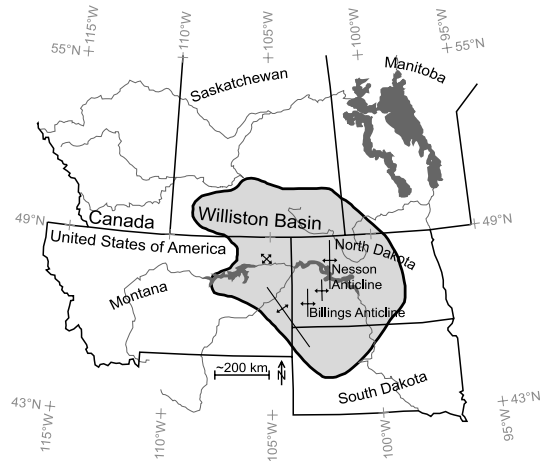
\includegraphics[scale=0.6]{bakken}
  }
  \caption{Расположение нефтегазоносного бассейна Уиллистон на границе США и Канады. Адаптировано с работы~\autocite{kuhn2012three}.}
  \label{fig:bakken}
\end{figure}

\begin{figure}[ht]
  \centerfloat{
    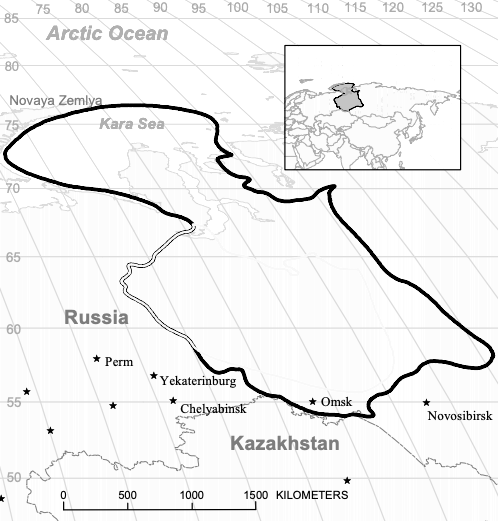
\includegraphics[scale=0.65]{bazhenov}
  }
  \caption{Расположение Баженовской свиты на территории Западной Сибири. Адаптировано с работы~\autocite{USGS}.}
  \label{fig:bazhenov}
\end{figure}

В то время как наличие естественных трещин является одной из ключевых характеристик в вопросах возможности добычи нефти и газа из низкопроницаемых пород, искусственные трещины, как правило образовавшиеся вследствие гидравлических разрывов (в англоязычной литературе устоялся термин OWHF или oil well hydraulic fracturing), лишь создают хоть сколько-нибудь проницаемую область (the SRV или Stimulated Reservoir Volume) в окрестности нефтедобывающей скважины~\autocite{warpinski2009stimulating}. Несмотря на бурное развитие технологий моделирования добычи нефти и газа из низкопроницаемых коллекторов в последнее двадцатилетие, известные математические модели не объясняют многие физические процессы в таких геологических породах. При непосредственной разработке таких резервуаров в среде проявляются различные нелинейные эффекты, нелинейные или не подчиняющиеся закону Дарси течения, а также так называемый Klinkenberg-эффект,~--- эффект прилипания/скольжения молекул газа (gas slip effect)  при течении в пористой среде. К числу перечисленных выше явлений также относят абсорбцию и десорбцию, сложное межмолекулярное взаимодействие (газ с водой, твердое тело с мелкими порами), трещинообразование. Вследствие этих нелинейных физических процессов и явлений, на сегодня в литературе имеет место быть лишь базовое представление о том, как движется нефть или газ в таких породах, и нет устоявшегося представления о том, как формируются и развиваются трещины в таких плотных неоднородных и неизотропных породах~\autocite{warpinski2009stimulating, wu2014generalized}.

Предлагаемая в данной работе модель двойной пористой среды с упругим трещиноватым скелетом дает физически качественное объяснение ряду физических процессов, связанных с аномально высоким пластовым давлением и трещинообразованием, и, как следствие, демонстрирует принципиальную возможность формирования подобной вышеописанной проницаемой области в окрестности скважины только благодаря аномально высокому пластовому давлению.

Давление в порах называется аномально высоким, если оно превышает гидростатический уровень. Аномально высокое пластовое давление, или АВПД (overpressure или abnormal pressure), является распространенным явлением в пластовых породах со сверхнизкой проницаемостью, таких как карбонаты, известняки и сланцы~\autocite{fertl1976abnormal, luo2002natural, melik1983, magara1978significance}. Выделяют несколько причин возникновения АВПД связанных с историей формирования залежи, термическим состоянием пласта, физико-химическими процессами, движением флюидов в земной коре. В частности, основным механизмом формирования АВПД в нефтематеринских породах является генерация флюида в условиях сверхнизкой проницаемости (созревание керогена в условиях низкой проницаемости). Аномально высокое пластовое давление достигает значений до 0.95 от горного давления~\autocite{li2012pore}, и может не только служить причиной разрушения стенок скважин~\autocite{melik1983, li2012pore}, но и способно поддерживать дебит нефти в низкопроницаемых коллекторах в отсутствие возможности применения традиционных методов поддержания пластового давления~\autocite{sonnenberg2009petroleum}. Кроме того, аномально высокое пластовое давление может приводить к развитию вторичных трещин в породе с низкой проницаемостью. Это явление, называемое автофлюидоразрыв или в англоязычной литературе как NHF (natural hydraulic fracturing), хорошо известно и обсуждается в связи с проблемой миграции флюидов~\autocite{secor1965role, engelder1990natural, luo2002natural}.

Первоначально концепция автофлюидоразрыва была развита в работах~\autocite{secor1965role} на основе подходов к моделированию традиционного гидроразрыва (OWHF). В~\autocite{secor1965role} рассматривается набор произвольно ориентированных трещин с непроницаемыми стенками на достаточно большом расстоянии друг от друга, чтобы исключить их взаимное влияние. В качестве критерия распространения трещин используется вариант энергетической теории Гриффитса. В дальнейшем эта модель была обобщена на случай пороупругой среды в предположении, что давление в трещинах в каждый момент времени равно поровому давлению в пространстве между трещинами~\autocite{engelder1990natural}. Указанные модели изначально сформулированы для описания развития трещиноватости в горных породах на геологических масштабах времени. При этом указывается, что автофлюидоразрыв играет важную роль в миграции флюидов. Например, если в силу определенных причин (например, созревание керогена в условиях низкой проницаемости) поровое давление в низкопроницаемом пласте, постепенно повышаясь, достигает критерия страгивания трещин (initiation), трещины начинают расти (propagation), что приводит к увеличению их объема, падению давления и, в результате, прекращению роста трещин (arrest). Процесс повторяется циклически. В работе~\autocite{luo2002natural} показано, что в сланцевых пластах при наличии АВПД возможно установление равновесия в окрестности критерия разрушения, когда генерируемый в нефтематеринской породе флюид отводится по системе трещин автофлюидоразрыва (зона I на рисунке~\ref{fig:NHF}).

В настоящей работе рассматривается ситуация, когда за длительный предшествующий период давление в матрице превысило гидростатический уровень, однако критерий разрушения еще не достигнут (например, зона II на рисунке~\ref{fig:NHF}). Считается, что разрушение в матрице может произойти при участии аномально высокого пластового давления в процессе технологических операций (например, бурение скважины, депрессия на забое скважины в процессе добычи и др.).

\begin{figure}[ht]
  \centerfloat{
    \includegraphics[scale=0.9]{NHF}
  }
  \caption{На следующем условном для данной работы рисунке (рисунок из~\autocite{luo2002natural}) по оси ординат сверху вниз отложено увеличение глубины, по абсцисс слева направо, - увеличение давления. Использованы следующие обозначения: [1]~--- аномально высокое пластовое давление, [2]~--- гидростатический уровень ($\rho g h$), [4]~--- условный критерий страгивания трещин, [3]~--- литостатический уровень.}
  \label{fig:NHF}
\end{figure}

Традиционно при описании движения флюидов в трещиновато-пористых коллекторах используют модель двойной пористости~\autocite{barenblatt1960basic, golf1986, wu2014generalized}. Такие трещиновато-пористые пласты состоят из блоков насыщенной пористой низкопроницаемой породы, называемой матрицей, разделенных магистральными трещинами, по которым двигается жидкость (см. рисунок~\ref{fig:barenblat}). При этом матрица осуществляет подпитку системы трещин. В основе семейства континуальных моделей среды с двойной пористостью, насыщенной одной жидкостью, лежит гипотеза суперпозиции трех континуумов (предполагается, что элементарный объем (REV или representative elementary volume), по которому проводится усреднение, много больше характерного расстояния между магистральными трещинами). Первый континуум образован частью жидкости, насыщающей матрицу, которая характеризуется низкой проницаемостью, но достаточно большой пористостью. Второй континуум образован жидкостью, заполняющей систему магистральных трещин, объемная доля которых мала по сравнению с пористостью матрицы. При этом проницаемость системы трещин предполагается достаточно высокой, чтобы обеспечить подвижность второго континуума. Третьим континуумом является твердый скелет, который может быть жестким, пороупругим или проявлять вязкие и пластические свойства. Стоит отметить, что, если блоки матрицы не изолированы, и проницаемость матрицы сравнима с проницаемостью трещин, модель двойной пористости часто называют моделью двойной проницаемости (и/или же моделью двойной проницаемости называют еще вследствие наличия разницы макроспкопических градиентов давлений между двумя подсистемами). Как правило, учет влияния аномально высокого пластового давления на производство нефти или газа в сланцевых породах сводится к учету зависимости проницаемости системы трещин в среде с двойной пористостью от давления~\autocite{thompson2010modeling} в связи с тем, что для движения флюидов в низкопроницаемых породах требуются значительные депрессии.

\begin{figure}[ht]
  \centerfloat{
    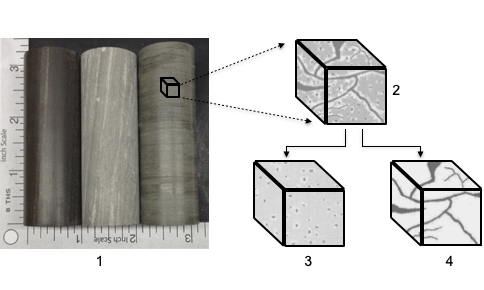
\includegraphics[scale=1]{comboimg}
  }
  \caption{Элементарный объем трещиноватой горной породы (2), состоящей из пор и проницаемых блоков (3), разделенных между собой системой трещин (4). (1)~--- три различных образца сланца из статьи~\autocite{ye2016fracture}. Адаптировано с работы~\autocite{abousleiman2005poromechanics}.}
  \label{fig:barenblat}
\end{figure}

В отличие от указанного подхода в данной работе развивается модель среды с двойной пористостью, матрица которой способна растрескиваться под действием аномально высокого пластового давления, тем самым увеличивая интенсивность массообмена между подсистемами матрицыи и трещины.

Развитие системы трещин, длина которых много меньше характерного размера элементарного объема, естественно моделировать методами теории повреждаемых сред (CDM~--- continuum damage mechanics)~\autocite{lemaitre2012course, murakami2012continuum}, в рамках которой коллектив микротрещин описывается осредненно с помощью специального параметра поврежденности. В настоящей работе для моделирования автофлюидоразрыва в матрице используется модель повреждаемости, аналогичная~\autocite{kondaurov2007, izvekov2009, izvekov2010}. Для простоты использован скалярный параметр поврежденности, что соответствует случайному распределению трещин по направлениям в пространстве. Критерий инициации начала развития повреждаемости в модели~\autocite{kondaurov2007, izvekov2009, izvekov2010} является своеобразным обобщением энергетического критерия Гриффитса на случай рассеянного разрушения хрупких сред. Предполагается, что возникающие микротрещины в матрице в первую очередь усиливают массообмен между матрицей и магистральными трещинами.



% {\progress}
% Этот раздел должен быть отдельным структурным элементом по
% ГОСТ, но он, как правило, включается в описание актуальности
% темы. Нужен он отдельным структурынм элемементом или нет ---
% смотрите другие диссертации вашего совета, скорее всего не нужен.

{\aim} данной работы является моделирование влияния аномально высокого пластового давления в двойной пористой среде с упругим трещиноватым скелетом.

Для~достижения поставленной цели необходимо было решить следующие {\tasks}:
\begin{enumerate}
  \item Разработать физическую модель, учитывающую аномально высокое пластовое давление в двойной пористой среде с упругим трещиноватым скелетом;
  \item Исследовать параметры модели, сделать численные оценки этих параметров;
  \item Провести численный расчет для рассматриваемой модели на примере задачи о производительности скважины.
\end{enumerate}


{\novelty}
\begin{enumerate}
  \item Учтено влияния аномально высокого пластового давления в двойной пористой среде, используя детерминистический параметр повреждаемости, таким образом матрица способна растрескиваться под действием аномально высокого пластового давления, - основное отличие от традиционных моделей двойной пористой среды;
  \item В отличие от работ концепции автофлюидоразрыва, в данной работе решается задача о производительности скважины, при этом рассматривается зона II на рисунке~\ref{fig:NHF}, когда за длительный предшествующий промежуток времени накопилось аномально высокое пластовое давление, но инициации развития трещин еще не было.
  \item Показаны закономерности работы скважины, в окрестности которой идут процессы разрушения за счет энергии накопленного аномально высокого пластового давления.
\end{enumerate}

%{\influence} \ldots

%{\methods} \ldots

%{\defpositions}
%\begin{enumerate}
%  \item Первое положение
%  \item Второе положение
%  \item Третье положение
%  \item Четвертое положение
%\end{enumerate}
%В папке Documents можно ознакомиться в решением совета из Томского ГУ
%в~файле \verb+Def_positions.pdf+, где обоснованно даются рекомендации
%по~формулировкам защищаемых положений.

%{\reliability} полученных результатов обеспечивается \ldots \ Результаты находятся в соответствии с результатами, %полученными другими авторами.


{\probation}
Основные результаты работы докладывались~на следующих конференциях:
\begin{enumerate}
  \item Международная конференция по геофизическим наукам (The EGU General Assembly), Вена, Австрия, 2019~\cite{eguconf}.
  \item Международная конференция по физике высоких температур и взаимодейтсвию материалов (XXXIV International Conference on Interaction of Intense Energy Fluxes with Matter), Эльбрус, Кабардино-Балкария, Россия, 2019~\cite{ivtanconf}.
  \item 61 научная конференция МФТИ, Долгопрудный, Россия, 2018~\cite{miptconf}.
\end{enumerate}

{\contribution} Автор принимал активное участие в обсуждении теоретических положений и алгоритма численного решения, а также в реализации алгоритма и интерпретации полученных результатов.

{\publications} Основные результаты по теме диссертации изложены в 1 научной статье,
каторая принята в печать журналом <<Физика Земли>>~\cite{fizzemli2020}.

% \ifnumequal{\value{bibliosel}}{0}
% {%%% Встроенная реализация с загрузкой файла через движок bibtex8. (При желании, внутри можно использовать обычные ссылки, наподобие `\cite{vakbib1,vakbib2}`).
%     {\publications} Основные результаты по теме диссертации изложены
%     в~XX~печатных изданиях,
%     X из которых изданы в журналах, рекомендованных ВАК,
%     X "--- в тезисах докладов.
% }%
% {%%% Реализация пакетом biblatex через движок biber
%     \begin{refsection}[bl-author]
%         % Это refsection=1.
%         % Процитированные здесь работы:
%         %  * подсчитываются, для автоматического составления фразы "Основные результаты ..."
%         %  * попадают в авторскую библиографию, при usefootcite==0 и стиле `\insertbiblioauthor` или `\insertbiblioauthorgrouped`
%         %  * нумеруются там в зависимости от порядка команд `\printbibliography` в этом разделе.
%         %  * при использовании `\insertbiblioauthorgrouped`, порядок команд `\printbibliography` в нём должен быть тем же (см. biblio/biblatex.tex)
%         %
%         % Невидимый библиографический список для подсчёта количества публикаций:
%         \printbibliography[heading=nobibheading, section=1, env=countauthorvak,          keyword=biblioauthorvak]%
%         \printbibliography[heading=nobibheading, section=1, env=countauthorwos,          keyword=biblioauthorwos]%
%         \printbibliography[heading=nobibheading, section=1, env=countauthorscopus,       keyword=biblioauthorscopus]%
%         \printbibliography[heading=nobibheading, section=1, env=countauthorconf,         keyword=biblioauthorconf]%
%         \printbibliography[heading=nobibheading, section=1, env=countauthorother,        keyword=biblioauthorother]%
%         \printbibliography[heading=nobibheading, section=1, env=countauthor,             keyword=biblioauthor]%
%         \printbibliography[heading=nobibheading, section=1, env=countauthorvakscopuswos, filter=vakscopuswos]%
%         \printbibliography[heading=nobibheading, section=1, env=countauthorscopuswos,    filter=scopuswos]%
%         %
%         \nocite{*}%
%         %
%         {\publications} Основные результаты по теме диссертации изложены в 1 печатном издании,
%         которое издано в журнале <<Физика Земли>> (Q2 по данным 2019 г.)~\cite{fizzemli2020}
%         % \ifnum \value{citeauthorconf}>0%
%             , 3 "--- в~тезисах докладов конференций.
%         % \else%
%             % .
%         % \fi
%     \end{refsection}%
%     \begin{refsection}[bl-author]
%         % Это refsection=2.
%         % Процитированные здесь работы:
%         %  * попадают в авторскую библиографию, при usefootcite==0 и стиле `\insertbiblioauthorimportant`.
%         %  * ни на что не влияют в противном случае
%         \nocite{vakbib2}%vak
%         \nocite{bib1}%other
%         \nocite{confbib1}%conf
%     \end{refsection}%
%         %
%         % Всё, что вне этих двух refsection, это refsection=0,
%         %  * для диссертации - это нормальные ссылки, попадающие в обычную библиографию
%         %  * для автореферата:
%         %     * при usefootcite==0, ссылка корректно сработает только для источника из `external.bib`. Для своих работ --- напечатает "[0]" (и даже Warning не вылезет).
%         %     * при usefootcite==1, ссылка сработает нормально. В авторской библиографии будут только процитированные в refsection=0 работы.
%         %
%         % Невидимый библиографический список для подсчёта количества внешних публикаций
%         % Используется, чтобы убрать приставку "А" у работ автора, если в автореферате нет
%         % цитирований внешних источников.
%         % Замедляет компиляцию
%     \ifsynopsis
%     \ifnumequal{\value{draft}}{0}{
%       %
%     }{}
%     \fi
%     \printbibliography[heading=nobibheading, section=0, env=countexternal,          keyword=biblioexternal]
% }
 % Характеристика работы по структуре во введении и в автореферате не отличается (ГОСТ Р 7.0.11, пункты 5.3.1 и 9.2.1), потому её загружаем из одного и того же внешнего файла, предварительно задав форму выделения некоторым параметрам

\textbf{Объем и структура работы.} Диссертация состоит из~введения, трёх глав и заключения.
%% на случай ошибок оставляю исходный кусок на месте, закомментированным
%Полный объём диссертации составляет  \ref*{TotPages}~страницу
%с~\totalfigures{}~рисунками и~\totaltables{}~таблицами. Список литературы
%содержит \total{citenum}~наименований.
%
Полный объём диссертации составляет
\formbytotal{TotPages}{страниц}{у}{ы}{}, включая
\formbytotal{totalcount@figure}{рисун}{ок}{ка}{ков} и
\formbytotal{totalcount@table}{таблиц}{у}{ы}{}.   Список литературы содержит
\formbytotal{citenum}{наименован}{ие}{ия}{ий}.
    % Введение
\ifnumequal{\value{contnumfig}}{1}{\counterwithout{figure}{chapter}
}{\counterwithin{figure}{chapter}}
\ifnumequal{\value{contnumtab}}{1}{\counterwithout{table}{chapter}
}{\counterwithin{table}{chapter}}
\chapter{Формулировка модели}\label{ch:ch1}

\section{Модель двойной пористости}\label{sec:ch1/sec00}

Рассмотрим насыщенную пористую среду с упругим хрупким скелетом, включающим пористую матрицу и систему магистральных трещин. Матрица имеет низкую проницаемость и относительно высокую пористость. Система трещин характеризуется высокой проницаемостью и низкой пористостью (относительный объем пустот, содержащихся в трещинах). Матрица и трещины насыщены одной и той же слабосжимаемой жидкостью. Блоки матрицы изолированы друг от друга в том смысле, что непосредственное перемещение жидкости из блока в блок отсутствует и может осуществляться только через систему трещин.

Будем рассматривать среду с двойной пористостью как суперпозицию трех сплошных сред~--- двух флюидов и скелета. Первый континуум (флюид) соответствует жидкости, находящейся в матрице, второй~--- жидкости, заполняющей магистральные трещины. Жидкость взаимодействует со скелетом посредством массовых сил вязкого трения и полагается вязкой сжимаемой. В настоящей работе всюду используется изотермическое приближение (это предположение является традиционным при моделировании нетепловых методов добычи нефти). Предполагается наличие умеренного массообмена между матрицей и трещинами (это означает, что поток между матрицей и трещинами мал по сравнению с потоком в трещинах). Все движения предполагаются квазистатическими (что позволяет пренебречь кинетической энергией и влиянием массообмена на импульс), а деформации скелета малыми. В задаче о производительности скважин характерные масштабы времени много меньше геологических, таким образом, возможной генерацией флюида в нефтематеринской породе можно пренебречь.

\section{Основные уравнения сохранения}\label{sec:ch1/sec01}

Выпишем основные уравнения в рамках сформулированных гипотез. Следствием законов сохранения массы являются три уравнения неразрывности, имеющие вид:

\begin{equation}
  \label{eq:masbalance1}
  \frac{\partial r_1}{\partial t} + \nabla \cdot (r_1 {\textbf{v}}_1 ) = \dot{m}_{12},
\end{equation}

\begin{equation}
  \label{eq:masbalance2}
  \frac{\partial r_2}{\partial t} + \nabla \cdot (r_2 {{\textbf{v}}}_2) = \dot{m}_{21},
\end{equation}

\begin{equation}
  \label{eq:masbalance3}
  \frac{\partial r_s}{\partial t} + \nabla \cdot (r_s {{\textbf{v}}}_s) = 0,
\end{equation}
где использованы индексы $1$, $2$, $S$ для обозначения величин, относящихся к флюиду, соответствующему жидкости в матрице, флюиду, соответствующему жидкости в трещинах, и к скелету соответственно. Также для обозначения величин, относящихся только к флюидам, используется индекс $\alpha$, а к любому из континуумов индекс $A$.

Тогда $\alpha = 1$ (матрица), $\alpha = 2$ (трещины), $r_{\alpha} = \rho_{f} \phi_{\alpha}$~--- плотность флюида как сплошной среды, $\rho_f$~--- истинная плотность флюида $\alpha$, $\phi_{\alpha}$~--- пористость (объемная доля пустот) матрицы и системы трещин: $\phi_{\alpha} = d V_{void}^{\alpha}/dV$ ($d V_{void}^{\alpha}$~--- объем, занимаемый жидкостью в подсистеме $\alpha$ (объем пустотного пространства), $d V$~--- элементарный объем), ${\textbf{v}}_{\alpha}$~--- скорость флюида, $\textbf{v}_{s}$~--- скорость скелета, плотность скелета как сплошной среды $r_s = (1 - \phi_1 - \phi_2) \rho_s$, $\rho_s$~--- истинная плотность скелета, $\dot{m}_{12} = -\dot{m}_{21}$ интенсивность массообмена между системами матриц и трещинами.

Уравнения движения флюида и скелета имеют следующий вид соответственно:
\begin{equation}
  \label{eq:motion1}
  r_{\alpha} \frac{d_{\alpha} \textbf{v}_{\alpha}}{d t} = - \phi_{\alpha} \nabla p_{\alpha} + r_{\alpha} {\textbf{g}} + \textbf{b}_{\alpha}^{dis} + \dot{m}_{\alpha \beta} \textbf{v}_{\alpha},
\end{equation}

\begin{equation}
  \label{eq:motion2}
  r_s \frac{d_s {\textbf{v}}_s}{d t} = \nabla \cdot {\textbf{T}}_s + r_s {\textbf{g}} + {\textbf{b}}_s^{int}.
\end{equation}

В данной модели уравнение движения жидкости преобразуется в закон Дарси:

\begin{equation}
  \label{eq:darcy}
  {\textbf{W}}_{\alpha} = - \frac{k_{\alpha}}{\mu_f} (\nabla p_{\alpha} + \rho_{\alpha}\textbf{g}),
\end{equation}
где вектор фильтрации ${\textbf{W}}_{\alpha} = \phi_{\alpha} ({\textbf{v}}_{\alpha} - {\textbf{v}}_s)$, $p_{\alpha}$~--- поровое давление, $k_{\alpha}$~--- проницаемость, $\mu_{\alpha}$~--- вязкость жидкости, $\textbf{g}$~--- ускорение свободного падения.

Предположим, что проницаемость матрицы стремится к нулю, т.е. $k_1 = 0$, а проницаемость трещин чувствительна к изменению давления $k_2 = k_2(p_2)$ (при этом $v_1 = v_s$).

Уравнение движения скелета~\eqref{eq:motion2} преобразуется в уравнение равновесия и тогда это уравнение можно записать как уравнение равновесия для скелета и флюидов как единого целого

\begin{equation}
  \label{eq:seqaulity}
  \nabla \cdot {\textbf{T}} = - r {\textbf{g}},
\end{equation}
здесь ${\textbf{T}} = {\textbf{T}}_s - (p_1 \phi_1 + p_2 \phi_2) \textbf{I}$~--- тензор полного напряжения в пористой среде, ${\textbf{T}}_s$~--- тензор парциальных напряжений в скелете, $p_{\alpha}$~--- поровое давление в подсистемах, $\textbf{I}$~--- единичный тензор второго ранга, $r = \sum_{A} {r_A}$.

\section{Определяющие соотношения}\label{sec:ch1/sec02}

Чтобы перейти непосредственно к замыкающим систему уравнений~\eqrefs{eq:masbalance1,eq:masbalance2,eq:masbalance3, eq:darcy, eq:seqaulity} определяющим (или по-другому реологическим) уравнениям, ниже будет выведено приведенное неравенство Клаузиуса-Дюгема в изотермическом приближении.

Сила трения между флюидами и скелетом, отнесенная к единице объема, имеет вид~\autocite{kondaurov2007, coussy2004poromechanics}:

\begin{equation}
  \label{eq:bint}
  \textbf{b}^{int}_{\alpha} = - p_{\alpha} \nabla \phi_{\alpha} + \textbf{b}^{dis}_{\alpha},
\end{equation}
где, в случае использования линейного закона течения в форме закона Дарси~\eqref{eq:darcy}, диссипативная часть этой силы взаимодействия равна

\begin{equation}
  \label{eq:bdis}
  \textbf{b}^{dis}_{\alpha} = - \frac{\mu_{\alpha}}{\phi_{\alpha} k_{\alpha}} \textbf{W}_{\alpha}.
\end{equation}

Дифференциальный закон сохранения энергии для элементарного тела, состоящего из частиц трех континуумов, с учетом уравнений баланса массы~\eqrefs{eq:masbalance1,eq:masbalance2,eq:masbalance3} и приведенных уравнений движения~\eqrefs{eq:darcy,eq:seqaulity} имеет вид

\begin{equation}
  \label{eq:difenergy}
  \sum_A{r_A \frac{d_A u_A}{dt}} = \sum_A{\textbf{T}_A : \nabla \otimes \textbf{v}_A} - \sum_A{\textbf{b}^{int}_{\alpha} \cdot \textbf{w}_{\alpha}} + rQ - \nabla \cdot \textbf{q} - \sum_{\alpha \neq \beta}{\dot{m}_{\alpha \beta} u_{\alpha}},
\end{equation}
здесь использованы оператор $d_A (\dots)/dt = \partial (\dots)/ \partial t + {\textbf{v}}_A \cdot \nabla \otimes (\dots)$~--- материальная Лагранжева производная вдоль траектории частиц континуума $A$ (знаком <<$\otimes$>> обозначено тензорное умножение), и двойное скалярное произведение ${\textbf{A} : \textbf{B}} = A_{ij} B_{ij}$, а также $u_A$~--- удельная внутренняя энергия, $q$~--- вектор суммарного теплового потока, $rQ$~--- суммарная мощность внешних источников тепла.

Для того же элементарного тела второе начало термодинамики в форме неравенства Клаузиуса-Дюгема с учетом массообмена имеет вид

\begin{equation}
  \label{eq:kd1}
  \sum{A}{r_A \frac{d_A \eta_A}{dt}}
  + \sum_{\alpha \neq \beta} {\eta_{\alpha} \dot{m}_{\alpha \beta}} + \nabla \left( \frac{\textbf{q}}{\theta} \right)  - \frac{rQ}{\theta} \geq 0,
\end{equation}
где $\eta_A$~--- удельная энтропия, $\theta$~--- температура континуумов.

Вводя удельную свободную энергию континуумов  и, исключая из~\eqref{eq:kd1} поток приведенного тепла с помощью~\eqref{eq:difenergy}, а также, используя уравнения сохранения~\eqrefs{eq:masbalance1, eq:masbalance2, eq:masbalance3, eq:darcy, eq:seqaulity}, получим приведенное неравенство Клаузиуса-Дюгема в изотермическом приближении:

\begin{equation}
  \label{eq:kdpriv}
  - \sum_A{r_A \frac{d_A \, \psi_A}{d t }}
  + {\textbf{T}}_{s} : \frac{d_s \, \textbf{e}}{d t } + \sum_{\alpha}{\left( p_{\alpha} \frac{d_s \, \phi_{\alpha}}{d t } + \frac{p_{\alpha} \phi_{\alpha}}{\rho_{\alpha}} \frac{d_{\alpha} \, \rho_{\alpha}}{d t} \right)} + \delta_w + \delta_m \geq 0,
\end{equation}
где тензор малой демормации обозначен соответственно $\textbf{e} = \frac{1}{2} (\nabla \otimes \textbf{u} + \nabla \otimes \textbf{u}^T)$, $\textbf{u}$~--- вектор перемещений частиц скелета, диссипация, связанная с фильтрацией флюидов:

$$
  \delta_w = - \sum_{\alpha} {\textbf{b}}_{\alpha}^{dis} \cdot {\textbf{w}}_{\alpha} = \sum_{\alpha}{\frac{\mu_{\alpha}}{k_{\alpha} \phi_{\alpha}}\textbf{W}_{\alpha}^2} \geq 0,
$$
диссипация, связанная с обменом массой между подсистемами:

$$
\delta_m = - \sum_{\alpha \neq \beta} \chi_{\alpha} \dot{m}_{\alpha, \beta},
$$
где $\chi_{\alpha} = \psi_{\alpha} + p_{\alpha}/\rho_{\alpha}$~--- свободная энергия Гиббса флюидов.

Далее для замыкания системы законов сохранения~\eqrefs{eq:masbalance1,eq:masbalance2,eq:masbalance3, eq:darcy, eq:seqaulity} сфорулируем систему термодинамически согласованных определяющих соотношений. Согласно теории развитой в~\autocite{trusdell1975} эти соотношения должны удовлетворять принципу детерминизма (утверждает, что реакция материала не зависит от будущих состояний), принципу локального действия (постулирует конечность
распространения возмущений в сплошной среде), принципу объективности (утверждает, что вид определяющих соотношений не должен зависеть от системы отсчета) и принципу термодинамической согласованности (утверждает, что
определяющие соотношения должны быть таковы, чтобы неравенство Клаузиса-Дюгема~\eqref{eq:kdpriv} выполнялось в произвольных процессах).

Определим понятия <<процесс>> и <<реакция>> в рассматриваемом случае двойной пороупругой среды с хрупким склетом. Сначала определим состояние материальной частицы пористой среды, как набор следующих параметров: тензор малой деформации $\textbf{e}$, плотности флюидов $\rho_{\alpha}$, относительная скорость флюидов и скелета $\textbf{w}_{\alpha}$, параметр поврежденности $\omega$. Параметр $\omega$ является внутренней переменной и в свернутом виде, накапливаясь, несет информацию о прошлых состояниях. Для новой внутренней переменной необходимо сформулировать кинетическое (эволюционное) уравнение. Предложенный набор термодинамических параметров соответствует предположению, что движение флюидов достаточно медленное, а площадь контакта флюида и стенок в скелете настолько большая, что можно пренебречь обменом импульсом внутри жидкости по сравнению с обменом импульсом между жидкостью и скелетом за счет вязкого трения. Сделанное предположение является традиционным для области применимости закона Дарси. В этом приближении флюиды, как сплошные среды, являются идеальными жидкостями, хотя составляющие их жидкости являются вязкими. Под <<процессом>> будем понимать последовательность смены параметров состояния, а под «реакцией» значения остальных неизвестных физических величин.

В общем виде, в рамках сделанных предположений, в качестве определяющих соотношений рассматриваемой среды примем набор функций, связывающих реакцию  с текущим состоянием пористой среды

\begin{equation}
  \label{eq:gamma1}
  \Gamma = \Gamma(\textbf{e}, \rho_{\alpha}, \textbf{w}_{\alpha}, \omega),
\end{equation}
где $\Gamma =  \{ \psi_{\alpha}, \textbf{T}_s, p_{\alpha}, \phi_{\alpha}, \dot{m}_{12}, \textbf{b}^{dis}_{\alpha} \}$. Эти соотношения~\eqref{eq:gamma1} должны быть дополнены кинетическим (эволюционным) уравнением на параметр поврежденности $\omega$:

\begin{equation}
  \label{eq:omega1}
  \frac{d_s \omega}{dt} = \Sigma (\textbf{e}, \rho_{\alpha}, \textbf{w}_{\alpha}, \omega),
\end{equation}
где $\Sigma$~--- функция текущего состояния среды.

Определяющие соотношения, необходимые и достаточные для выполнения~\eqref{eq:kdpriv} в произвольном процессе имеют следующий вид для флюидов:

\begin{equation}
  \label{eq:equationfluid}
        \begin{aligned}
                \psi_{\alpha} &= \psi_{\alpha} (\rho_{\alpha}), \\
                p_{\alpha} &= \rho_{\alpha}^2 \frac{\partial \psi_{\alpha}}{\partial \rho_{\alpha}} \\
        \end{aligned}
\end{equation}
и для скелета соответственно:

\begin{equation}
  \label{eq:equationskelet}
        \begin{aligned}
                {\textbf{T}} &= r_s \frac{\partial \Psi}{\partial \textbf{e}}, \\
                \phi_{\alpha} &= -r_s \frac{\partial \Psi}{\partial p_{\alpha}}. \\
        \end{aligned}
\end{equation}

В определяющих соотношениях~\eqref{eq:equationskelet} использован потенциал скелета

$$
\Psi (\textbf{e}_s, p_{\alpha}, \omega ) = F - \sum_{\alpha}{\frac{p_{\alpha}}{\rho_s} \phi_{\alpha}}, 
$$
согласно~\autocite{kondaurov2007}, где $F(\textbf{e}_s, \phi_{\alpha}, \omega) = \psi_s (\textbf{e}_s, \phi_{\alpha}(\textbf{e}_s, \rho_{\alpha}, \omega), \omega)$.

С учетом предложенных выше релогических соотношений~\eqrefs{eq:equationfluid, eq:equationskelet} неравенство Клаузиуса-Дюгема~\eqref{eq:kdpriv} принимает вид неравенства диссипаций:

\begin{equation}
  \label{eq:dissipneq}
  \delta_{\omega} + \delta_w + \delta_m \geq 0,
\end{equation}
где $\delta_{\omega} = - \left( \frac{\partial \Psi}{\partial \omega} \frac{d_s \omega}{d t} \right) = - \left( \frac{\partial \Psi}{\partial \omega} \right) \Sigma$~---- диссипация, связанная с растрескиванием матрицы.

Процедура доказательства соотношений~\eqrefs{eq:equationfluid, eq:equationskelet, eq:dissipneq} во многом аналогична, используемой в~\autocite{kondaurov2007}, и здесь не приводится.

Далее примем гипотезу, что каждая диссипация в отдельности неотрицательна, что является достаточным условием для выполнения~\eqref{eq:dissipneq}:

\begin{equation}
  \label{eq:dissipneq2}
  \delta_{\omega} \geq 0, \, \delta_w \geq 0, \, \delta_m \geq 0,
\end{equation}

\section{Линеаризация}\label{sec:ch1/sec03}

Чтобы использовать определяющие соотношения для скелета~\eqref{eq:equationskelet}, необходимо определить вид потенциала скелета $\Psi$. Для этого линеаризуем полученные определяющие соотношения в окрестности особого состояния: скелет не деформирован, жидкости покоятся, давления флюидов $p_1^0 = p_2^0 = 0$, т.е. $\{ 0, \rho_{\alpha}, 0, \omega \}$ . Давления во флюидах и напряжения в скелете в произвольных состояниях будем считать малыми по сравнению с характерными упругими модулями скелета $p_{\alpha}/K \ll 1, |\textbf{T}_s|/K \ll 1$, где $K$~--- модуль объемного сжатия скелета. Также рассмотрим частный случай, в котором начальные полные напряжения в состоянии  $ \{ 0, \rho_{\alpha}, 0, 0 \} $ равны нулю (в общем случае это не так, см.~\autocite{muha2018}).

Разложение свободной энергии в ряд по малому параметру $ \delta p_{\alpha} / \rho_{\alpha}^0 \ll 1$ до квадратичных членов в окрестности состояния $\{ 0, \rho_{\alpha}^0, 0, \omega \}$ имеет следующий вид

\begin{equation}
  \label{eq:freeseries}
  \rho_{\alpha} \psi_{\alpha} (\rho_{\alpha}) = \psi_{\alpha}^0 + p_{\alpha}^0 \left( \frac{\delta p_{\alpha}}{\rho_{\alpha}^0}\right) + \frac{1}{2} K_f \left( \frac{\delta p_{\alpha}}{\rho_{\alpha}^0} \right)^2,
\end{equation}
где $K_f$~--- модуль объемного сжатия жидкости. После подстановки в определяющие соотношения для флюида~\eqref{eq:equationfluid} дает линейное определяющее соотношение

\begin{equation}
  \label{eq:equationfluidnext}
  \frac{\delta \rho_{\alpha}}{\rho_{\alpha}^0} = \frac{\delta p_{\alpha}}{K_f}.
\end{equation}

Вслед за~\autocite{kondaurov2007, izvekov2009, izvekov2010} положим, что влияние поврежденности на упругие модули пренебрежимо мало. При этом макроскопическим проявлением поврежденности становится остаточная деформация в поврежденном материале, что формально сближает данный вариант модели повреждаемости с теорией пластичности. Скелет будем считать изотропным. Представим разложение потенциала скелета до величин второго порядка малости, считая      поврежденность $\omega$ одним из малых параметров, в следующем виде

\begin{equation}
 \label{eq:skeletseries}
   \begin{multlined}
       r_s^0 \Psi({\textbf{e}}, p_{\alpha}, \omega) = \frac{1}{2}\lambda I_1^2 + \mu J^2 + \sum_{\alpha} b_{\alpha} p_{\alpha} I_1 + \\
       + \sum_{\alpha} \frac{1}{2 N_{\alpha} } p_{\alpha}^2+ \frac{1}{N_{12}} p_1 p_2 + \sum_{\alpha}\phi_{\alpha}^0 p_{\alpha} + \gamma \omega + \beta \omega^2/2 - \\
       - \alpha I_1 \omega - \alpha_J J \omega - \alpha_{p_1} p_1\omega - \alpha_{p_2} p_2 \omega + \dots,
   \end{multlined}
\end{equation}
где $\lambda, \mu$~--- коффициенты Ламе скелета; $\textbf{I}_1 = \textbf{e} : \textbf{I}$, $\textbf{J} = \sqrt{\textbf{e}' : \textbf{e}'}$, $\textbf{e}'$~--- девиатор тензора малых деформаций; $b_{\alpha}$ и $N_{\alpha}$~--- аналоги коэффициентов Био и модуля Био для матрицы и трещин; $N_{12}$~--- модуль, отвечающий за взаимное влияние поровых давлений в подсистемах, $\alpha \geq 0, \alpha_J \geq 0, \alpha_{p1} \geq 0, \alpha_{p2} \leq 0$~--- коэффициенты, отвечающие за разгрузку упругой энергии при развитии поврежденности, $\gamma, \beta$~--- положительные коэффициенты, задающие нелинейную зависимость от поврежденности нулевого члена разложения упругой энергии скелета, характеризующего затраты энергии на появление новых поверхностей.

Подстановка~\eqref{eq:skeletseries} в~\eqref{eq:equationskelet} дает линейные определяющие соотношения для скелета

\begin{equation}
  \label{eq:linequationskelet1}
  \textbf{T} = \left( \textbf{K} \textbf{I}_1 - \sum_{\alpha}{b_{\alpha}p_{\alpha} - \alpha \omega} \right) \textbf{I} + \left( 2\mu - \frac{\alpha_J \omega}{J} \right) \textbf{e}',
\end{equation}

\begin{equation}
  \label{eq:linequationskelet2}
  \phi_1 = \phi_1^0 + (b_1 - \phi_1^0) \textbf{I}_1 + \frac{p_1}{N_1} + \frac{p_2}{N_{12}} + \alpha_{p1} \omega,
\end{equation}

\begin{equation}
  \label{eq:linequationskelet3}
  \phi_2 = \phi_2^0 + (b_2 - \phi_2^0) \textbf{I}_1 + \frac{p_2}{N_2} + \frac{p_2}{N_{12}} + \alpha_{p2} \omega,
\end{equation}
где $K = \lambda + \frac{2}{3} \mu$~--- модуль объемного сжатия скелета.

Обсудим неравенства диссипаций~\eqref{eq:dissipneq2}. Учтем, что, согласно сделанным предположениям относительно начального состояния флюидов, $\psi_1^0 = \psi_2^0$, тогда справедлива следующая оценка

\begin{equation}
  \label{eq:approxdeltam}
  \delta_m = - \sum_{\alpha \neq \beta}{\psi_{\alpha} + \frac{p_{\alpha}}{\rho_{\alpha}}\dot{m}_{\alpha \beta}} \approx - \sum_{alpha \neq \beta}{\frac{p_{\alpha}}{\rho_{\alpha}}\dot{m}_{\alpha \beta}} \approx \frac{\dot{m}}{\rho_2^0}(p_1 - p_2) \geq 0,
\end{equation}
где введено обозначение $\dot{m} = - \dot{m}_{12} = \dot{m}_{21}$. Величина $\dot{m} \geq 0$, если матрица подпитывает трещины. Удовлетворим неравенству~\eqref{eq:approxdeltam} с помощью простого уравнения, задающего закон обмена массой между флюидами

\begin{equation}
  \label{eq:intensofm}
  \dot{m} = \frac{\rho^0}{\mu_f} A(\omega)(p_1 - p_2),
\end{equation}
где $A(\omega) \geq 0$~--- коэффициент, определяющий интенсивность массообмена. В результате растрескивания улучшается возможность транспорта жидкости внутри матрицы, что проявляется в усилении массообмена между флюидами. В случае неповрежденной матрицы~\eqref{eq:intensofm} совпадает с классическим выражением~\autocite{barenblatt1960basic}.

Поступая аналогично~\autocite{kondaurov2007, izvekov2009, izvekov2010} примем следующий закон эволюции поврежденности, достаточный для удовлетворения неравенству диссипации $\delta_{\omega} \geq 0$

\begin{equation}
  \label{eq:evalomega}
  \frac{\partial \omega}{\partial t} = -\frac{r_s}{\tau \beta} \left\langle \frac{\partial \Psi}{\partial \omega} \right\rangle,
  \left\langle x \right\rangle =
  \begin{cases}
    x, \text{если } x \geqslant 0, \\
    0, \text{если } x<0,
  \end{cases}
\end{equation}
где $\tau$~--- характерное время запаздывания разрушения, $\beta$~--- размерный параметр.

Физический смысл выражения~\eqref{eq:evalomega} заключается в том, что поврежденность развивается только в том случае, когда упругая энергия, высвобождающаяся при появлении новых поверхностей, превышает энергозатраты на их появление. Чем сильнее эта разница, тем интенсивнее развивается поврежденность. Уравнение~\eqref{eq:evalomega} является в некотором роде аналогом теории Гриффитса для изолированной трещины.

Подставляя в~\eqref{eq:evalomega} представление потенциала скелета~\eqref{eq:skeletseries}, получим следующее линейное эволюционное уравнение на параметр повреждаемости

\begin{equation}
  \label{eq:evalomega1}
  \frac{\partial \omega}{\partial t} = \frac{1}{\tau \beta} \left\langle  \alpha I_1 + \alpha_J J + \alpha_{p_1} p_1 + \alpha_{p_2} p_2 -\beta \omega - \gamma \right\rangle.
\end{equation}

Эволюция параметров однородного гидростатического напряженного состояния при отсутствии обмена между подсистемами описывается системой уравнений, следующих из~\eqrefs{eq:masbalance1, eq:masbalance2, eq:seqaulity}, с учетом~\eqrefs{eq:linequationskelet1, eq:linequationskelet2, eq:linequationskelet3, eq:evalomega1}:

\begin{equation}
  \label{eq:linequationskelet4}
  \textbf{K} \textbf{I}_1 - b_1 p_1 - b_2 p_2 - \alpha \omega = C,
\end{equation}

\begin{equation}
  \label{eq:linequationskelet5}
  \left( \frac{1}{N_1} + \frac{\phi_1^0}{K_F} + \frac{b_1^2}{K} \right) \frac{\partial p_1}{\partial t} + \left( \frac{1}{N_{12}} + \frac{b_1 b_2}{K} \right) \frac{\partial p_2}{\partial t} + \left( \alpha_{p1} + \frac{\alpha b_1}{K} \right) \frac{\partial \omega}{\partial t} = 0,
\end{equation}

\begin{equation}
  \label{eq:linequationskelet6}
  \left( \frac{1}{N_2} + \frac{\phi_2^0}{K_F} + \frac{b_2^2}{K} \right) \frac{\partial p_1}{\partial t} + \left( \frac{1}{N_{12}} + \frac{b_1 b_2}{K} \right) \frac{\partial p_1}{\partial t} + \left( \alpha_{p2} + \frac{\alpha b_2}{K} \right) \frac{\partial \omega}{\partial t} = 0,
\end{equation}

\begin{equation}
 \label{eq:linequationskelet7}
   \begin{multlined}
     \tau \frac{\partial \omega}{\partial t} = \left( K^{-1} \frac{\alpha^2}{\beta} - 1 \right) \omega + \frac{1}{\beta} \left( \alpha_{p1} + \frac{\alpha b_1}{K} \right) p_1 +
     \\
     + \frac{1}{\beta} \left( \alpha_{p2} + \frac{\alpha b_2}{K} \right) p_2 + \frac{1}{\beta} \left( \frac{\alpha C}{K} - \gamma \right).
   \end{multlined}
\end{equation}

Решение данной системы имеет вид $\textbf{x} = \textbf{a} e^{\Gamma t } + \textbf{b}$, где $x=(I_1, p_1, p_2, \omega)^T$, $\textbf{a} = const, \textbf{b}=const$.

Система неравенств

\begin{equation}
  \label{eq:neq1}
  \frac{\alpha^2}{\beta} < K,
\end{equation}

\begin{equation}
  \label{eq:neq2}
  \left( \frac{1}{N_{12}} + \frac{b_1 b_2}{K} \right)^2 < \left( \frac{1}{N_1} + \frac{\phi_1^0}{K_f} + \frac{b_1^2}{K} \right) \left( \frac{1}{N_2} + \frac{\phi_2^0}{K_f} + \frac{b_2^2}{K} \right),
\end{equation}
является достаточным условием выполнения неравенства в показателе степени решения $\Gamma < 0$.  В дальнейшем эти ограничения на коэффициенты модели, гарантирующие устойчивость однородного напряженного состояния, считаются выполненными.

Из ограниченности скорости  $\partial \omega / \partial t$ при $\tau \rightarrow 0 $, из~\eqref{eq:evalomega1} следует выражение для параметра $\omega$

\begin{equation}
  \label{eq:omeganext}
  \omega = \max_{[0,t]} \left( \frac{1}{\beta} (\alpha I_1 + \alpha_J J + \alpha_{p_1} p_1 + \alpha_{p_2} p_2 -\beta \omega - \gamma) \right).
\end{equation}

Из выражения~\eqref{eq:evalomega1} следует критерий начала накопления поврежденности. Одновременное выполнение условий $\partial \omega / \partial t \geq 0$ и $\omega = 0$ дает для границы зоны упругого поведения в пространстве инвариантов тензора малой деформации следующее уравнение

\begin{equation}
  \label{eq:eq34}
  \alpha I_1 + \alpha_J J + \alpha_{p_1} p_1 + \alpha_{p_2} p_2 -\beta \omega - \gamma = 0.
\end{equation}

Условие $\alpha I_1 + \alpha_J J + \alpha_{p_1} p_1 + \alpha_{p_2} p_2 -\beta \omega - \gamma < 0$ соответствует упругому поведению. При выполнении условия  $\alpha I_1 + \alpha_J J + \alpha_{p_1} p_1 + \alpha_{p_2} p_2 -\beta \omega - \gamma > 0$ возможны активный процесс ($\partial \omega / \partial t > 0$) и упругая разгрузка (пассивный процесс). В пассивном процессе полагается $\omega = 0$.






% \section{Форматирование текста}\label{sec:ch1/sec1}

% Мы можем сделать \textbf{жирный текст} и \textit{курсив}.

% \section{Ссылки}\label{sec:ch1/sec2}

% Сошлёмся на библиографию.
% Одна ссылка: \cite[с.~54]{Sokolov}\cite[с.~36]{Gaidaenko}.
% Две ссылки: \cite{Sokolov,Gaidaenko}.
% Ссылка на собственные работы: \cite{vakbib1, confbib2}.
% Много ссылок: %\cite[с.~54]{Lermontov,Management,Borozda} % такой «фокус»
% %вызывает biblatex warning относительно опции sortcites, потому что неясно, к
% %какому источнику относится уточнение о страницах, а bibtex об этой проблеме
% %даже не предупреждает
% \cite{Lermontov, Management, Borozda, Marketing, Constitution, FamilyCode,
% Gost.7.0.53, Razumovski, Lagkueva, Pokrovski, Methodology, Nasirova, Berestova,
% Kriger}%
% \ifnumequal{\value{bibliosel}}{0}{% Примеры для bibtex8
%     \cite{Sirotko, Lukina, Encyclopedia}%
% }{% Примеры для biblatex через движок biber
%     \cite{Sirotko2, Lukina2, Encyclopedia2}%
% }%
% .
% И~ещё немного ссылок:~\cite{Article,Book,Booklet,Conference,Inbook,Incollection,Manual,Mastersthesis,
% Misc,Phdthesis,Proceedings,Techreport,Unpublished}
% % Следует обратить внимание, что пробел после запятой внутри \cite{}
% % обрабатывается ожидаемо, а пробел перед запятой, может вызывать проблемы при
% % обработке ссылок.
% \cite{medvedev2006jelektronnye, CEAT:CEAT581, doi:10.1080/01932691.2010.513279,
% Gosele1999161,Li2007StressAnalysis, Shoji199895, test:eisner-sample,
% test:eisner-sample-shorted, AB_patent_Pomerantz_1968, iofis_patent1960}
% \ifnumequal{\value{bibliosel}}{0}{% Примеры для bibtex8
% }{% Примеры для biblatex через движок biber
%     \cite{patent2h, patent3h, patent2}%
% }%
% .

% \ifnumequal{\value{bibliosel}}{0}{% Примеры для bibtex8
% Попытка реализовать несколько ссылок на конкретные страницы
% для \texttt{bibtex} реализации библиографии:
% [\citenum{Sokolov}, с.~54; \citenum{Gaidaenko}, с.~36].
% }{% Примеры для biblatex через движок biber
% Несколько источников (мультицитата):
% % Тут специально написано по-разному тире, для демонстрации, что
% % применение специальных тире в настоящий момент в biblatex приводит к непоказу
% % "с.".
% \cites[vii--x, 5, 7]{Sokolov}[v"--~x, 25, 526]{Gaidaenko}[vii--x, 5, 7]{Techreport},
% работает только в \texttt{biblatex} реализации библиографии.
% }%

% Ссылки на собственные работы:~\cite{vakbib1, confbib1}

% Сошлёмся на приложения: Приложение~\ref{app:A}, Приложение~\ref{app:B2}.

% Сошлёмся на формулу: формула~\eqref{eq:equation1}.

% Сошлёмся на изображение: рисунок~\ref{fig:knuth}.

% Стандартной практикой является добавление к ссылкам префикса, характеризующего тип элемента.
% Это не является строгим требованием, но~позволяет лучше ориентироваться в документах большого размера.
% Например, для ссылок на~рисунки используется префикс \textit{fig},
% для ссылки на~таблицу "--- \textit{tab}.

% В таблице~\ref{tab:tab_pref} приложения~\ref{app:B4} приведён список рекомендуемых
% к использованию стандартных префиксов.

% \section{Формулы}\label{sec:ch1/sec3}

% Благодаря пакету \textit{icomma}, \LaTeX~одинаково хорошо воспринимает
% в~качестве десятичного разделителя и запятую (\(3,1415\)), и точку (\(3.1415\)).

% \subsection{Ненумерованные одиночные формулы}\label{subsec:ch1/sec3/sub1}

% Вот так может выглядеть формула, которую необходимо вставить в~строку
% по~тексту: \(x \approx \sin x\) при \(x \to 0\).

% А вот так выглядит ненумерованная отдельностоящая формула c подстрочными
% и надстрочными индексами:
% \[
% (x_1+x_2)^2 = x_1^2 + 2 x_1 x_2 + x_2^2
% \]

% Формула с неопределенным интегралом:
% \[
% \int f(\alpha+x)=\sum\beta
% \]

% При использовании дробей формулы могут получаться очень высокие:
% \[
%   \frac{1}{\sqrt{2}+
%   \displaystyle\frac{1}{\sqrt{2}+
%   \displaystyle\frac{1}{\sqrt{2}+\cdots}}}
% \]

% В формулах можно использовать греческие буквы:
% %Все \original... команды заранее, ради этого примера, определены в Dissertation\userstyles.tex
% \[
% \alpha\beta\gamma\delta\originalepsilon\epsilon\zeta\eta\theta%
% \vartheta\iota\kappa\varkappa\lambda\mu\nu\xi\pi\varpi\rho\varrho%
% \sigma\varsigma\tau\upsilon\originalphi\phi\chi\psi\omega\Gamma\Delta%
% \Theta\Lambda\Xi\Pi\Sigma\Upsilon\Phi\Psi\Omega
% \]
% \[%https://texfaq.org/FAQ-boldgreek
% \boldsymbol{\alpha\beta\gamma\delta\originalepsilon\epsilon\zeta\eta%
% \theta\vartheta\iota\kappa\varkappa\lambda\mu\nu\xi\pi\varpi\rho%
% \varrho\sigma\varsigma\tau\upsilon\originalphi\phi\chi\psi\omega\Gamma%
% \Delta\Theta\Lambda\Xi\Pi\Sigma\Upsilon\Phi\Psi\Omega}
% \]

% Для добавления формул можно использовать пары \verb+$+\dots\verb+$+ и \verb+$$+\dots\verb+$$+,
% но~они считаются устаревшими.
% Лучше использовать их функциональные аналоги \verb+\(+\dots\verb+\)+ и \verb+\[+\dots\verb+\]+.

% \subsection{Ненумерованные многострочные формулы}\label{subsec:ch1/sec3/sub2}

% Вот так можно написать две формулы, не нумеруя их, чтобы знаки <<равно>> были
% строго друг под другом:
% \begin{align}
%   f_W & =  \min \left( 1, \max \left( 0, \frac{W_{soil} / W_{max}}{W_{crit}} \right)  \right), \nonumber \\
%   f_T & =  \min \left( 1, \max \left( 0, \frac{T_s / T_{melt}}{T_{crit}} \right)  \right), \nonumber
% \end{align}

% Выровнять систему ещё и по переменной \( x \) можно, используя окружение
% \verb|alignedat| из пакета \verb|amsmath|. Вот так:
% \[
%     |x| = \left\{
%     \begin{alignedat}{2}
%         &&x, \quad &\text{eсли } x\geqslant 0 \\
%         &-&x, \quad & \text{eсли } x<0
%     \end{alignedat}
%     \right.
% \]
% Здесь первый амперсанд (в исходном \LaTeX\ описании формулы) означает
% выравнивание по~левому краю, второй "--- по~\( x \), а~третий "--- по~слову
% <<если>>. Команда \verb|\quad| делает большой горизонтальный пробел.

% Ещё вариант:
% \[
%     |x|=
%     \begin{cases}
%     \phantom{-}x, \text{если } x \geqslant 0 \\
%     -x, \text{если } x<0
%     \end{cases}
% \]

% Кроме того, для  нумерованных формул \verb|alignedat| делает вертикальное
% выравнивание номера формулы по центру формулы. Например, выравнивание
% компонент вектора:
% \begin{equation}
% \label{eq:2p3}
% \begin{alignedat}{2}
% {\mathbf{N}}_{o1n}^{(j)} = \,{\sin} \phi\,n\!\left(n+1\right)
%          {\sin}\theta\,
%          \pi_n\!\left({\cos} \theta\right)
%          \frac{
%               z_n^{(j)}\!\left( \rho \right)
%               }{\rho}\,
%           &{\boldsymbol{\hat{\mathrm e}}}_{r}\,+   \\
% +\,
% {\sin} \phi\,
%          \tau_n\!\left({\cos} \theta\right)
%          \frac{
%             \left[\rho z_n^{(j)}\!\left( \rho \right)\right]^{\prime}
%               }{\rho}\,
%             &{\boldsymbol{\hat{\mathrm e}}}_{\theta}\,+   \\
% +\,
% {\cos} \phi\,
%          \pi_n\!\left({\cos} \theta\right)
%          \frac{
%             \left[\rho z_n^{(j)}\!\left( \rho \right)\right]^{\prime}
%               }{\rho}\,
%             &{\boldsymbol{\hat{\mathrm e}}}_{\phi}\:.
% \end{alignedat}
% \end{equation}

% Ещё об отступах. Иногда для лучшей <<читаемости>> формул полезно
% немного исправить стандартные интервалы \LaTeX\ с учётом логической
% структуры самой формулы. Например в формуле~\ref{eq:2p3} добавлен
% небольшой отступ \verb+\,+ между основными сомножителями, ниже
% результат применения всех вариантов отступа:
% \begin{align*}
% \backslash! &\quad f(x) = x^2\! +3x\! +2 \\
%   \mbox{по-умолчанию} &\quad f(x) = x^2+3x+2 \\
% \backslash, &\quad f(x) = x^2\, +3x\, +2 \\
% \backslash{:} &\quad f(x) = x^2\: +3x\: +2 \\
% \backslash; &\quad f(x) = x^2\; +3x\; +2 \\
% \backslash \mbox{space} &\quad f(x) = x^2\ +3x\ +2 \\
% \backslash \mbox{quad} &\quad f(x) = x^2\quad +3x\quad +2 \\
% \backslash \mbox{qquad} &\quad f(x) = x^2\qquad +3x\qquad +2
% \end{align*}

% Можно использовать разные математические алфавиты:
% \begin{align}
% \mathcal{ABCDEFGHIJKLMNOPQRSTUVWXYZ} \nonumber \\
% \mathfrak{ABCDEFGHIJKLMNOPQRSTUVWXYZ} \nonumber \\
% \mathbb{ABCDEFGHIJKLMNOPQRSTUVWXYZ} \nonumber
% \end{align}

% Посмотрим на систему уравнений на примере аттрактора Лоренца:

% \[
% \left\{
%   \begin{array}{rl}
%     \dot x = & \sigma (y-x) \\
%     \dot y = & x (r - z) - y \\
%     \dot z = & xy - bz
%   \end{array}
% \right.
% \]

% А для вёрстки матриц удобно использовать многоточия:
% \[
% \left(
%   \begin{array}{ccc}
%     a_{11} & \ldots & a_{1n} \\
%     \vdots & \ddots & \vdots \\
%     a_{n1} & \ldots & a_{nn} \\
%   \end{array}
% \right)
% \]

% \subsection{Нумерованные формулы}\label{subsec:ch1/sec3/sub3}

% А вот так пишется нумерованная формула:
% \begin{equation}
%   \label{eq:equation1}
%   e = \lim_{n \to \infty} \left( 1+\frac{1}{n} \right) ^n
% \end{equation}

% Нумерованных формул может быть несколько:
% \begin{equation}
%   \label{eq:equation2}
%   \lim_{n \to \infty} \sum_{k=1}^n \frac{1}{k^2} = \frac{\pi^2}{6}
% \end{equation}

% Впоследствии на формулы~\eqref{eq:equation1} и~\eqref{eq:equation2} можно ссылаться.

% Сделать так, чтобы номер формулы стоял напротив средней строки, можно,
% используя окружение \verb|multlined| (пакет \verb|mathtools|) вместо
% \verb|multline| внутри окружения \verb|equation|. Вот так:
% \begin{equation} % \tag{S} % tag - вписывает свой текст
%   \label{eq:equation3}
%     \begin{multlined}
%         1+ 2+3+4+5+6+7+\dots + \\
%         + 50+51+52+53+54+55+56+57 + \dots + \\
%         + 96+97+98+99+100=5050
%     \end{multlined}
% \end{equation}

% Используя команду \verb|\eqrefs|, можно
% красиво ссылаться сразу на несколько формул
% \eqrefs{eq:equation1, eq:equation3, eq:equation2}, даже перепутав
% порядок ссылок \verb|\eqrefs{eq1, eq3, eq2}|.
% Аналогично, для ссылок на несколько рисунков, таблиц и~т.\:д.
% \refs{sec:ch1/sec1, sec:ch1/sec2, sec:ch1/sec3} можно использовать
% команду \verb|\refs|.
% Обе эти команды определены в файле \verb|common/packages.tex|.

% Уравнения~\eqrefs{eq:subeq_1,eq:subeq_2} демонстрируют возможности
% окружения \verb|\subequations|.
% \begin{subequations}
%     \label{eq:subeq_1}
%     \begin{gather}
%         y = x^2 + 1 \label{eq:subeq_1-1} \\
%         y = 2 x^2 - x + 1 \label{eq:subeq_1-2}
%     \end{gather}
% \end{subequations}
% Ссылки на отдельные уравнения~\eqrefs{eq:subeq_1-1,eq:subeq_1-2,eq:subeq_2-1}.
% \begin{subequations}
%     \label{eq:subeq_2}
%     \begin{align}
%         y &= x^3 + x^2 + x + 1 \label{eq:subeq_2-1} \\
%         y &= x^2
%     \end{align}
% \end{subequations}

% \subsection{Форматирование чисел и размерностей величин}\label{sec:units}

% Числа форматируются при помощи команды \verb|\num|:
% \num{5,3};
% \num{2,3e8};
% \num{12345,67890};
% \num{2,6 d4};
% \num{1+-2i};
% \num{.3e45};
% \num[exponent-base=2]{5 e64};
% \num[exponent-base=2,exponent-to-prefix]{5 e64};
% \num{1.654 x 2.34 x 3.430}
% \num{1 2 x 3 / 4}.
% Для написания последовательности чисел можно использовать команды \verb|\numlist| и \verb|\numrange|:
% \numlist{10;30;50;70}; \numrange{10}{30}.
% Значения углов можно форматировать при помощи команды \verb|\ang|:
% \ang{2.67};
% \ang{30,3};
% \ang{-1;;};
% \ang{;-2;};
% \ang{;;-3};
% \ang{300;10;1}.

% Обратите внимание, что ГОСТ запрещает использование знака <<->> для обозначения отрицательных чисел
% за исключением формул, таблиц и~рисунков.
% Вместо него следует использовать слово <<минус>>.

% Размерности можно записывать при помощи команд \verb|\si| и \verb|\SI|:
% \si{\farad\squared\lumen\candela};
% \si{\joule\per\mole\per\kelvin};
% \si[per-mode = symbol-or-fraction]{\joule\per\mole\per\kelvin};
% \si{\metre\per\second\squared};
% \SI{0.10(5)}{\neper};
% \SI{1.2-3i e5}{\joule\per\mole\per\kelvin};
% \SIlist{1;2;3;4}{\tesla};
% \SIrange{50}{100}{\volt}.
% Список единиц измерений приведён в таблицах~\refs{tab:unit:base,
% tab:unit:derived,tab:unit:accepted,tab:unit:physical,tab:unit:other}.
% Приставки единиц приведены в~таблице~\ref{tab:unit:prefix}.

% С дополнительными опциями форматирования можно ознакомиться в~описании пакета \texttt{siunitx};
% изменить или добавить единицы измерений можно в~файле \texttt{siunitx.cfg}.

% \begin{table}
%     \centering
%     \captionsetup{justification=centering} % выравнивание подписи по-центру
%     \caption{Основные величины СИ}\label{tab:unit:base}
%     \begin{tabular}{llc}
%         \toprule
%         Название  & Команда                & Символ         \\
%         \midrule
%         Ампер     & \verb|\ampere| & \si{\ampere}   \\
%         Кандела   & \verb|\candela| & \si{\candela}  \\
%         Кельвин   & \verb|\kelvin| & \si{\kelvin}   \\
%         Килограмм & \verb|\kilogram| & \si{\kilogram} \\
%         Метр      & \verb|\metre| & \si{\metre}    \\
%         Моль      & \verb|\mole| & \si{\mole}     \\
%         Секунда   & \verb|\second| & \si{\second}   \\
%         \bottomrule
%     \end{tabular}
% \end{table}

% \begin{table}
%   \small
%   \centering
%   \begin{threeparttable}% выравнивание подписи по границам таблицы
%     \caption{Производные единицы СИ}\label{tab:unit:derived}
%     \begin{tabular}{llc|llc}
%         \toprule
%         Название       & Команда                 & Символ              & Название & Команда & Символ \\
%         \midrule
%         Беккерель      & \verb|\becquerel|  & \si{\becquerel}     &
%         Ньютон         & \verb|\newton|  & \si{\newton}                                      \\
%         Градус Цельсия & \verb|\degreeCelsius| & \si{\degreeCelsius} &
%         Ом             & \verb|\ohm| & \si{\ohm}                                         \\
%         Кулон          & \verb|\coulomb| & \si{\coulomb}       &
%         Паскаль        & \verb|\pascal| & \si{\pascal}                                      \\
%         Фарад          & \verb|\farad| & \si{\farad}         &
%         Радиан         & \verb|\radian| & \si{\radian}                                      \\
%         Грей           & \verb|\gray| & \si{\gray}          &
%         Сименс         & \verb|\siemens| & \si{\siemens}                                     \\
%         Герц           & \verb|\hertz| & \si{\hertz}         &
%         Зиверт         & \verb|\sievert| & \si{\sievert}                                     \\
%         Генри          & \verb|\henry| & \si{\henry}         &
%         Стерадиан      & \verb|\steradian| & \si{\steradian}                                   \\
%         Джоуль         & \verb|\joule| & \si{\joule}         &
%         Тесла          & \verb|\tesla| & \si{\tesla}                                       \\
%         Катал          & \verb|\katal| & \si{\katal}         &
%         Вольт          & \verb|\volt| & \si{\volt}                                        \\
%         Люмен          & \verb|\lumen| & \si{\lumen}         &
%         Ватт           & \verb|\watt| & \si{\watt}                                        \\
%         Люкс           & \verb|\lux| & \si{\lux}           &
%         Вебер          & \verb|\weber| & \si{\weber}                                       \\
%         \bottomrule
%     \end{tabular}
%   \end{threeparttable}
% \end{table}

% \begin{table}
%   \centering
%   \begin{threeparttable}% выравнивание подписи по границам таблицы
%     \caption{Внесистемные единицы}\label{tab:unit:accepted}

%     \begin{tabular}{llc}
%         \toprule
%         Название        & Команда                 & Символ          \\
%         \midrule
%         День            & \verb|\day| & \si{\day}       \\
%         Градус          & \verb|\degree| & \si{\degree}    \\
%         Гектар          & \verb|\hectare| & \si{\hectare}   \\
%         Час             & \verb|\hour| & \si{\hour}      \\
%         Литр            & \verb|\litre| & \si{\litre}     \\
%         Угловая минута  & \verb|\arcminute| & \si{\arcminute} \\
%         Угловая секунда & \verb|\arcsecond| & \si{\arcsecond} \\ %
%         Минута          & \verb|\minute| & \si{\minute}    \\
%         Тонна           & \verb|\tonne| & \si{\tonne}     \\
%         \bottomrule
%     \end{tabular}
%   \end{threeparttable}
% \end{table}

% \begin{table}
%     \centering
%     \captionsetup{justification=centering}
%     \caption{Внесистемные единицы, получаемые из эксперимента}\label{tab:unit:physical}
%     \begin{tabular}{llc}
%         \toprule
%         Название                & Команда                 & Символ                 \\
%         \midrule
%         Астрономическая единица & \verb|\astronomicalunit| & \si{\astronomicalunit} \\
%         Атомная единица массы   & \verb|\atomicmassunit| & \si{\atomicmassunit}   \\
%         Боровский радиус        & \verb|\bohr| & \si{\bohr}             \\
%         Скорость света          & \verb|\clight| & \si{\clight}           \\
%         Дальтон                 & \verb|\dalton| & \si{\dalton}           \\
%         Масса электрона         & \verb|\electronmass| & \si{\electronmass}     \\
%         Электрон Вольт          & \verb|\electronvolt| & \si{\electronvolt}     \\
%         Элементарный заряд      & \verb|\elementarycharge| & \si{\elementarycharge} \\
%         Энергия Хартри          & \verb|\hartree| & \si{\hartree}          \\
%         Постоянная Планка       & \verb|\planckbar| & \si{\planckbar}        \\
%         \bottomrule
%     \end{tabular}
% \end{table}

% \begin{table}
%   \centering
%   \begin{threeparttable}% выравнивание подписи по границам таблицы
%     \caption{Другие внесистемные единицы}\label{tab:unit:other}
%     \begin{tabular}{llc}
%         \toprule
%         Название                  & Команда                 & Символ             \\
%         \midrule
%         Ангстрем                  & \verb|\angstrom| & \si{\angstrom}     \\
%         Бар                       & \verb|\bar| & \si{\bar}          \\
%         Барн                      & \verb|\barn| & \si{\barn}         \\
%         Бел                       & \verb|\bel| & \si{\bel}          \\
%         Децибел                   & \verb|\decibel| & \si{\decibel}      \\
%         Узел                      & \verb|\knot| & \si{\knot}         \\
%         Миллиметр ртутного столба & \verb|\mmHg| & \si{\mmHg}         \\
%         Морская миля              & \verb|\nauticalmile| & \si{\nauticalmile} \\
%         Непер                     & \verb|\neper| & \si{\neper}        \\
%         \bottomrule
%     \end{tabular}
%   \end{threeparttable}
% \end{table}

% \begin{table}
%   \small
%   \centering
%   \begin{threeparttable}% выравнивание подписи по границам таблицы
%     \caption{Приставки СИ}\label{tab:unit:prefix}
%     \begin{tabular}{llcc|llcc}
%         \toprule
%         Приставка & Команда                 & Символ      & Степень &
%         Приставка & Команда                 & Символ      & Степень   \\
%         \midrule
%         Иокто     & \verb|\yocto| & \si{\yocto} & -24     &
%         Дека      & \verb|\deca| & \si{\deca}  & 1         \\
%         Зепто     & \verb|\zepto| & \si{\zepto} & -21     &
%         Гекто     & \verb|\hecto| & \si{\hecto} & 2         \\
%         Атто      & \verb|\atto| & \si{\atto}  & -18     &
%         Кило      & \verb|\kilo| & \si{\kilo}  & 3         \\
%         Фемто     & \verb|\femto| & \si{\femto} & -15     &
%         Мега      & \verb|\mega| & \si{\mega}  & 6         \\
%         Пико      & \verb|\pico| & \si{\pico}  & -12     &
%         Гига      & \verb|\giga| & \si{\giga}  & 9         \\
%         Нано      & \verb|\nano| & \si{\nano}  & -9      &
%         Терра     & \verb|\tera| & \si{\tera}  & 12        \\
%         Микро     & \verb|\micro| & \si{\micro} & -6      &
%         Пета      & \verb|\peta| & \si{\peta}  & 15        \\
%         Милли     & \verb|\milli| & \si{\milli} & -3      &
%         Екса      & \verb|\exa| & \si{\exa}   & 18        \\
%         Санти     & \verb|\centi| & \si{\centi} & -2      &
%         Зетта     & \verb|\zetta| & \si{\zetta} & 21        \\
%         Деци      & \verb|\deci| & \si{\deci}  & -1      &
%         Иотта     & \verb|\yotta| & \si{\yotta} & 24        \\
%         \bottomrule
%     \end{tabular}
%   \end{threeparttable}
% \end{table}

% \subsection{Заголовки с формулами: \texorpdfstring{\(a^2 + b^2 = c^2\)}{%
% a\texttwosuperior\ + b\texttwosuperior\ = c\texttwosuperior},
% \texorpdfstring{\(\left\vert\textrm{{Im}}\Sigma\left(
% \protect\varepsilon\right)\right\vert\approx const\)}{|ImΣ (ε)| ≈ const},
% \texorpdfstring{\(\sigma_{xx}^{(1)}\)}{σ\_\{xx\}\textasciicircum\{(1)\}}
% }\label{subsec:with_math}

% Пакет \texttt{hyperref} берёт текст для закладок в pdf-файле из~аргументов
% команд типа \verb|\section|, которые могут содержать математические формулы,
% а~также изменения цвета текста или шрифта, которые не отображаются в~закладках.
% Чтобы использование формул в заголовках не вызывало в~логе компиляции появление
% предупреждений типа <<\texttt{Token not allowed in~a~PDF string
% (Unicode):(hyperref) removing...}>>, следует использовать конструкцию
% \verb|\texorpdfstring{}{}|, где в~первых фигурных скобках указывается
% формула, а~во~вторых "--- запись формулы для закладок.

% \section{Рецензирование текста}\label{sec:markup}

% В шаблоне для диссертации и автореферата заданы команды рецензирования.
% Они видны при компиляции шаблона в режиме черновика или при установке
% соответствующей настройки (\verb+showmarkup+) в~файле \verb+common/setup.tex+.

% Команда \verb+\todo+ отмечает текст красным цветом.
% \todo{Например, так.}

% Команда \verb+\note+ позволяет выбрать цвет текста.
% \note{Чёрный, } \note[red]{красный, } \note[green]{зелёный, }
% \note[blue]{синий.} \note[orange]{Обратите внимание на ширину и расстановку
% формирующихся пробелов, в~результате приведённой записи (зависит также
% от~применяемого компилятора).}

% Окружение \verb+commentbox+ также позволяет выбрать цвет.

% \begin{commentbox}[red]
%         Красный текст.

%         Несколько параграфов красного текста.
% \end{commentbox}

% \begin{commentbox}[blue]
%         Синяя формула.

%         \begin{equation}
%                 \alpha + \beta = \gamma
%         \end{equation}
% \end{commentbox}

% \verb+commentbox+ позволяет закомментировать участок кода в~режиме чистовика.
% Чтобы убрать кусок кода для всех режимов, можно использовать окружение
% \verb+comment+.

% \begin{comment}
%         Этот текст всегда скрыт.
% \end{comment}

\FloatBarrier
           % Глава 1
\chapter{Оценка параметров модели}\label{ch:ch2}

\section{Оценка пороупругих коэффициентов}\label{sec:ch2/sec01}

Выяснению физического смысла и способам лабораторного определения пороупругих констант для среды с двойной пористостью посвящен ряд работ~\autocite{berryman2002models, bai1995poromechanical}. Существуют также обобщения пороупругой модели на случай мульти-пористости~\autocite{mehrabian2015gassmann}. Приведем здесь простые оценки относительных значений коэффициентов $b_1$ и $b_2$, модулей $N_{\alpha}$ и $N_{12}$, подвергнув среду одноосному сжатию с нулевой поперечной деформацией. Соответствующая приближенная одномерная эквивалентная схема состоит из двух последовательно соединенных герметичных камер (элементов схемы). В ненапряженном состоянии продольные размеры камер равны $l_1^0$ и $l_2^0$, причем $l_2^0 \ll l_1^0$, как показано на рисунке~\ref{fig:coef1-1}. Торцевые стенки камер могут скользить без трения вдоль горизонтальной оси. Первая камера, играющая роль матрицы, заполнена пороупругой средой с пористостью $n_1$, упругим модулем $E_1$, коэффициентом Био $\alpha_1$ и модулем Био $\widetilde{N}$. Внутри второй камеры, соответствующей магистральным трещинам, находится пружина жесткостью $E_2$ (считаем, что трещины не заполнены ничем, кроме жидкости). Обозначим $\xi_{\alpha} = \frac{l_{\alpha}}{l_1^0 + l_2^0}$ объемные доли матрицы и трещин, так что $\xi_1 + \xi_2 = 1$. Объемные доли флюидов (<<пористости>>) будут равны $\phi_1 = n_1 \xi_1, phi_2 = n_2 \xi_2$. В камеры независимо нагнетаются давления $p_1$ и $p_2$.

\begin{figure}[ht]
    \centerfloat{
        \hfill
        \subcaptionbox[List-of-Figures entry]{\label{fig:coef1-1}}{%
            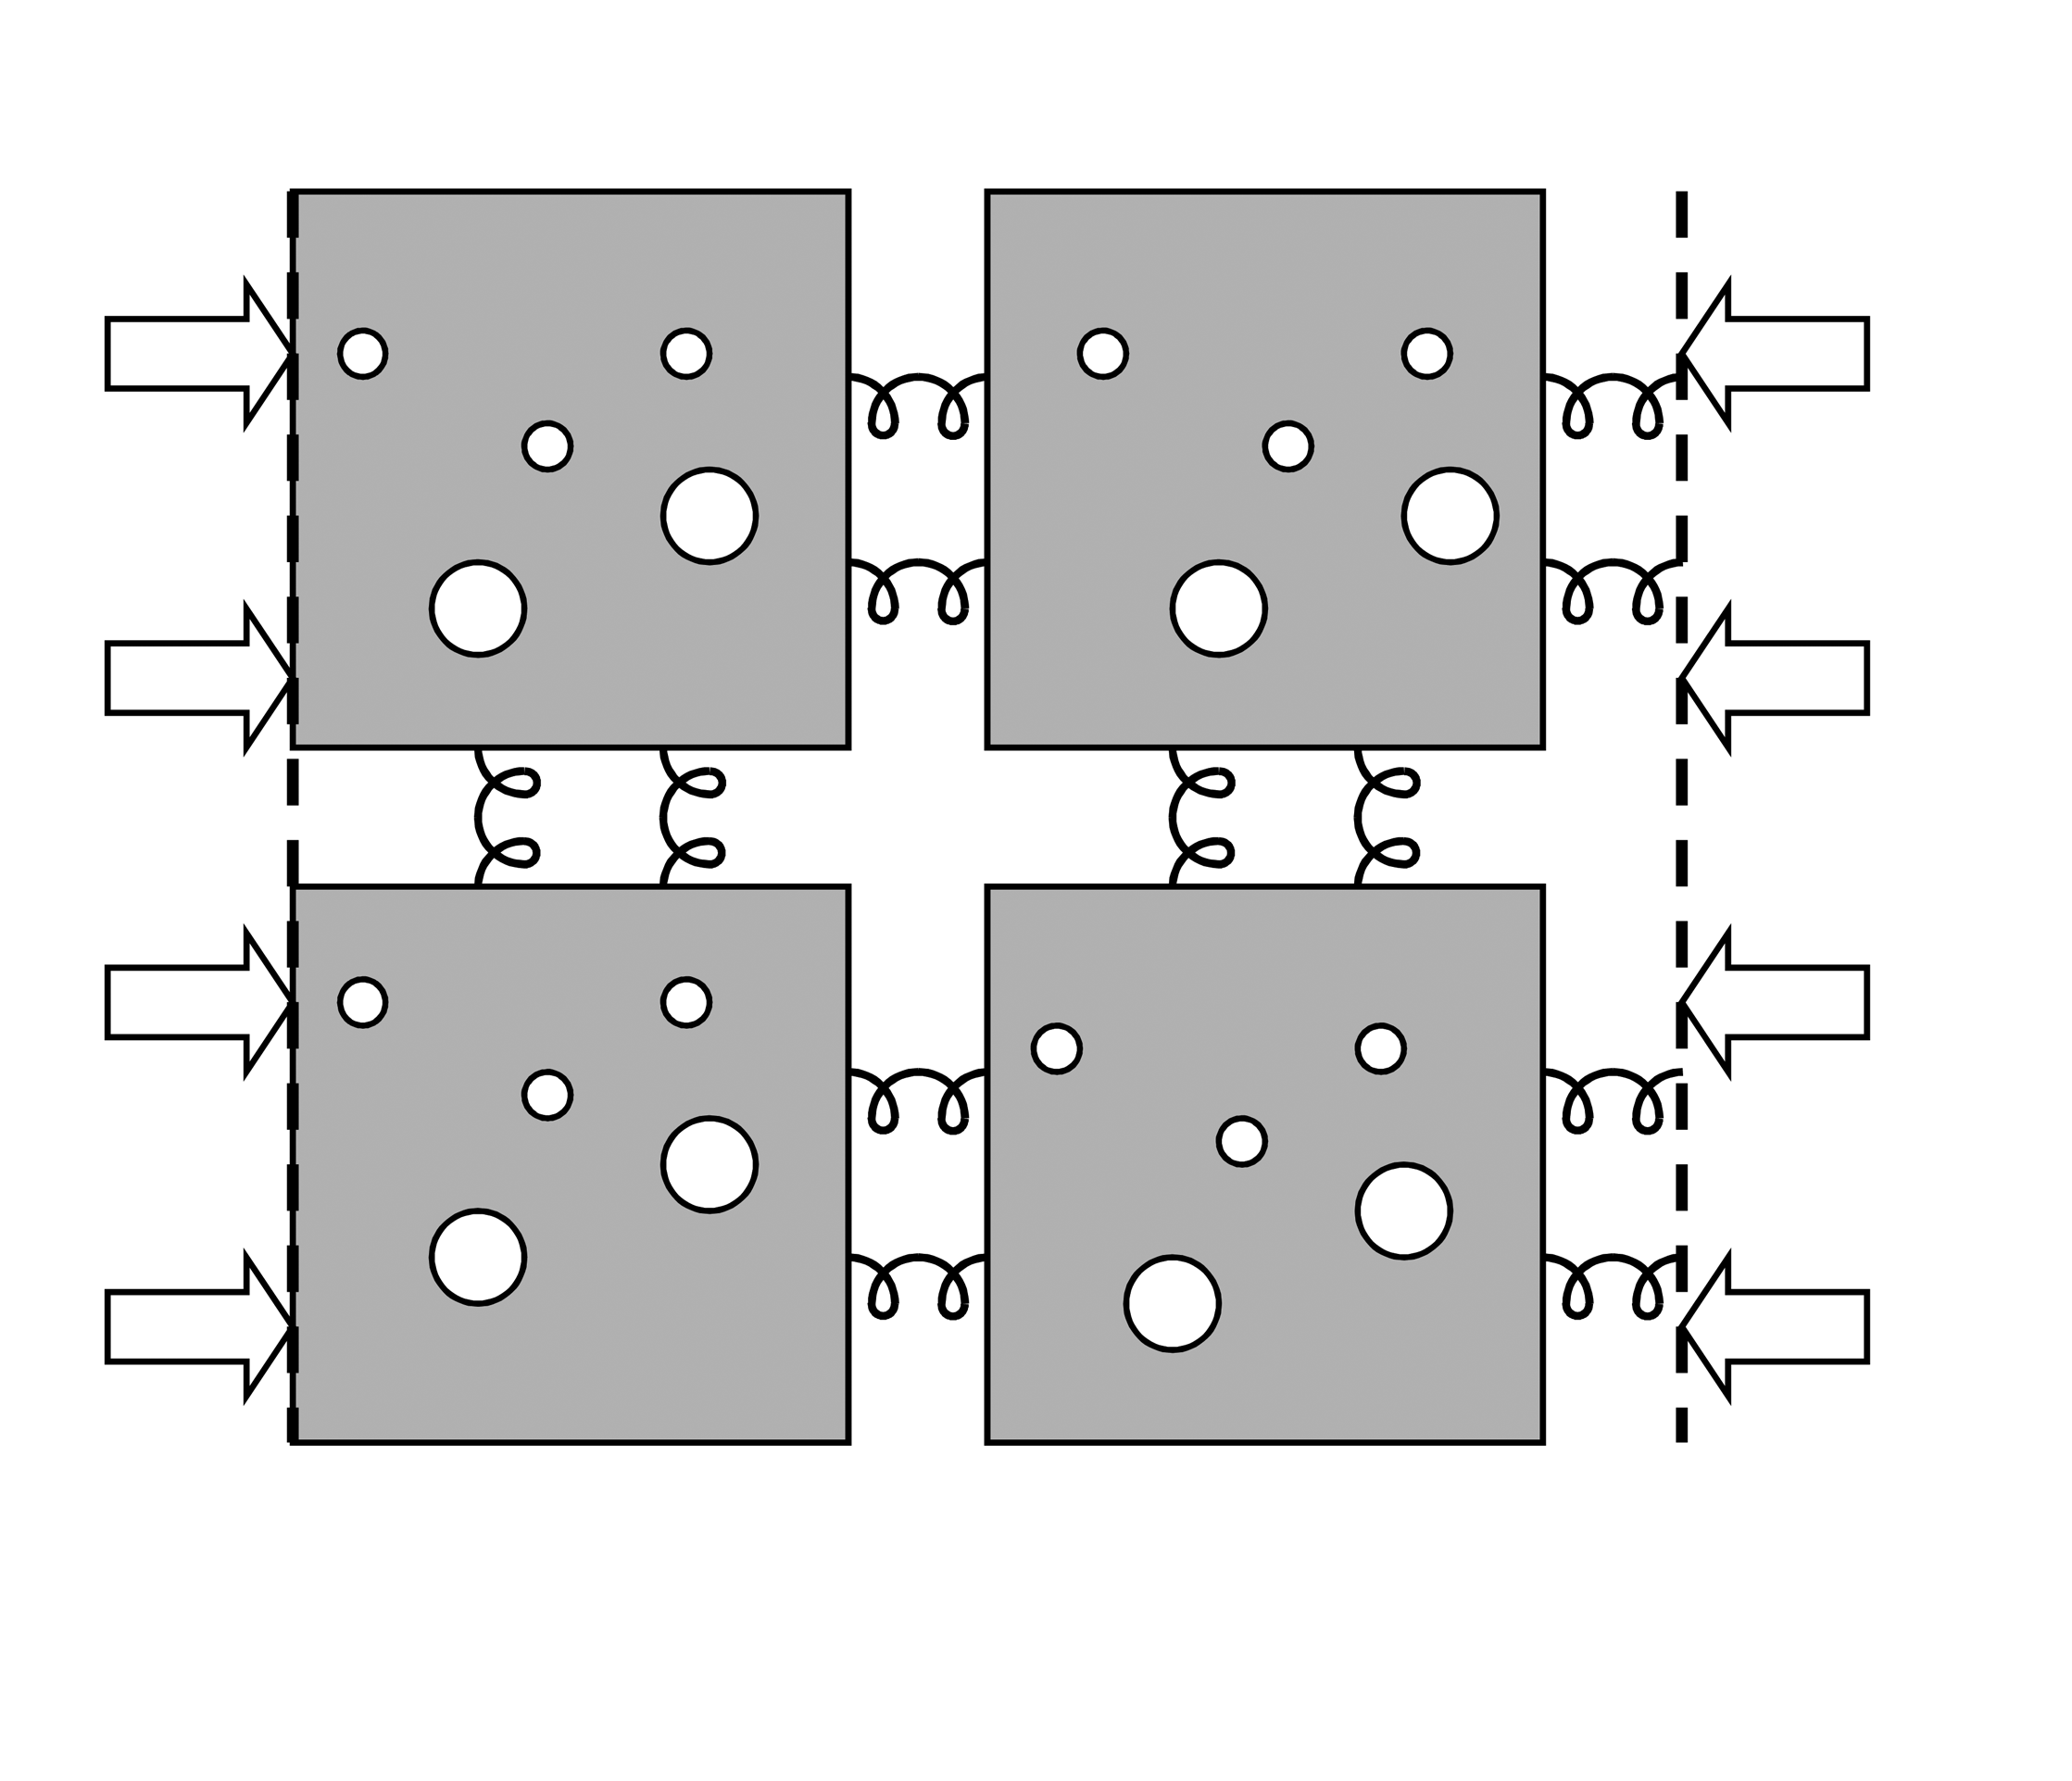
\includegraphics[width=0.4\linewidth]{coef1}}
        \hfill
        \subcaptionbox{\label{fig:coef1-2}}{%
            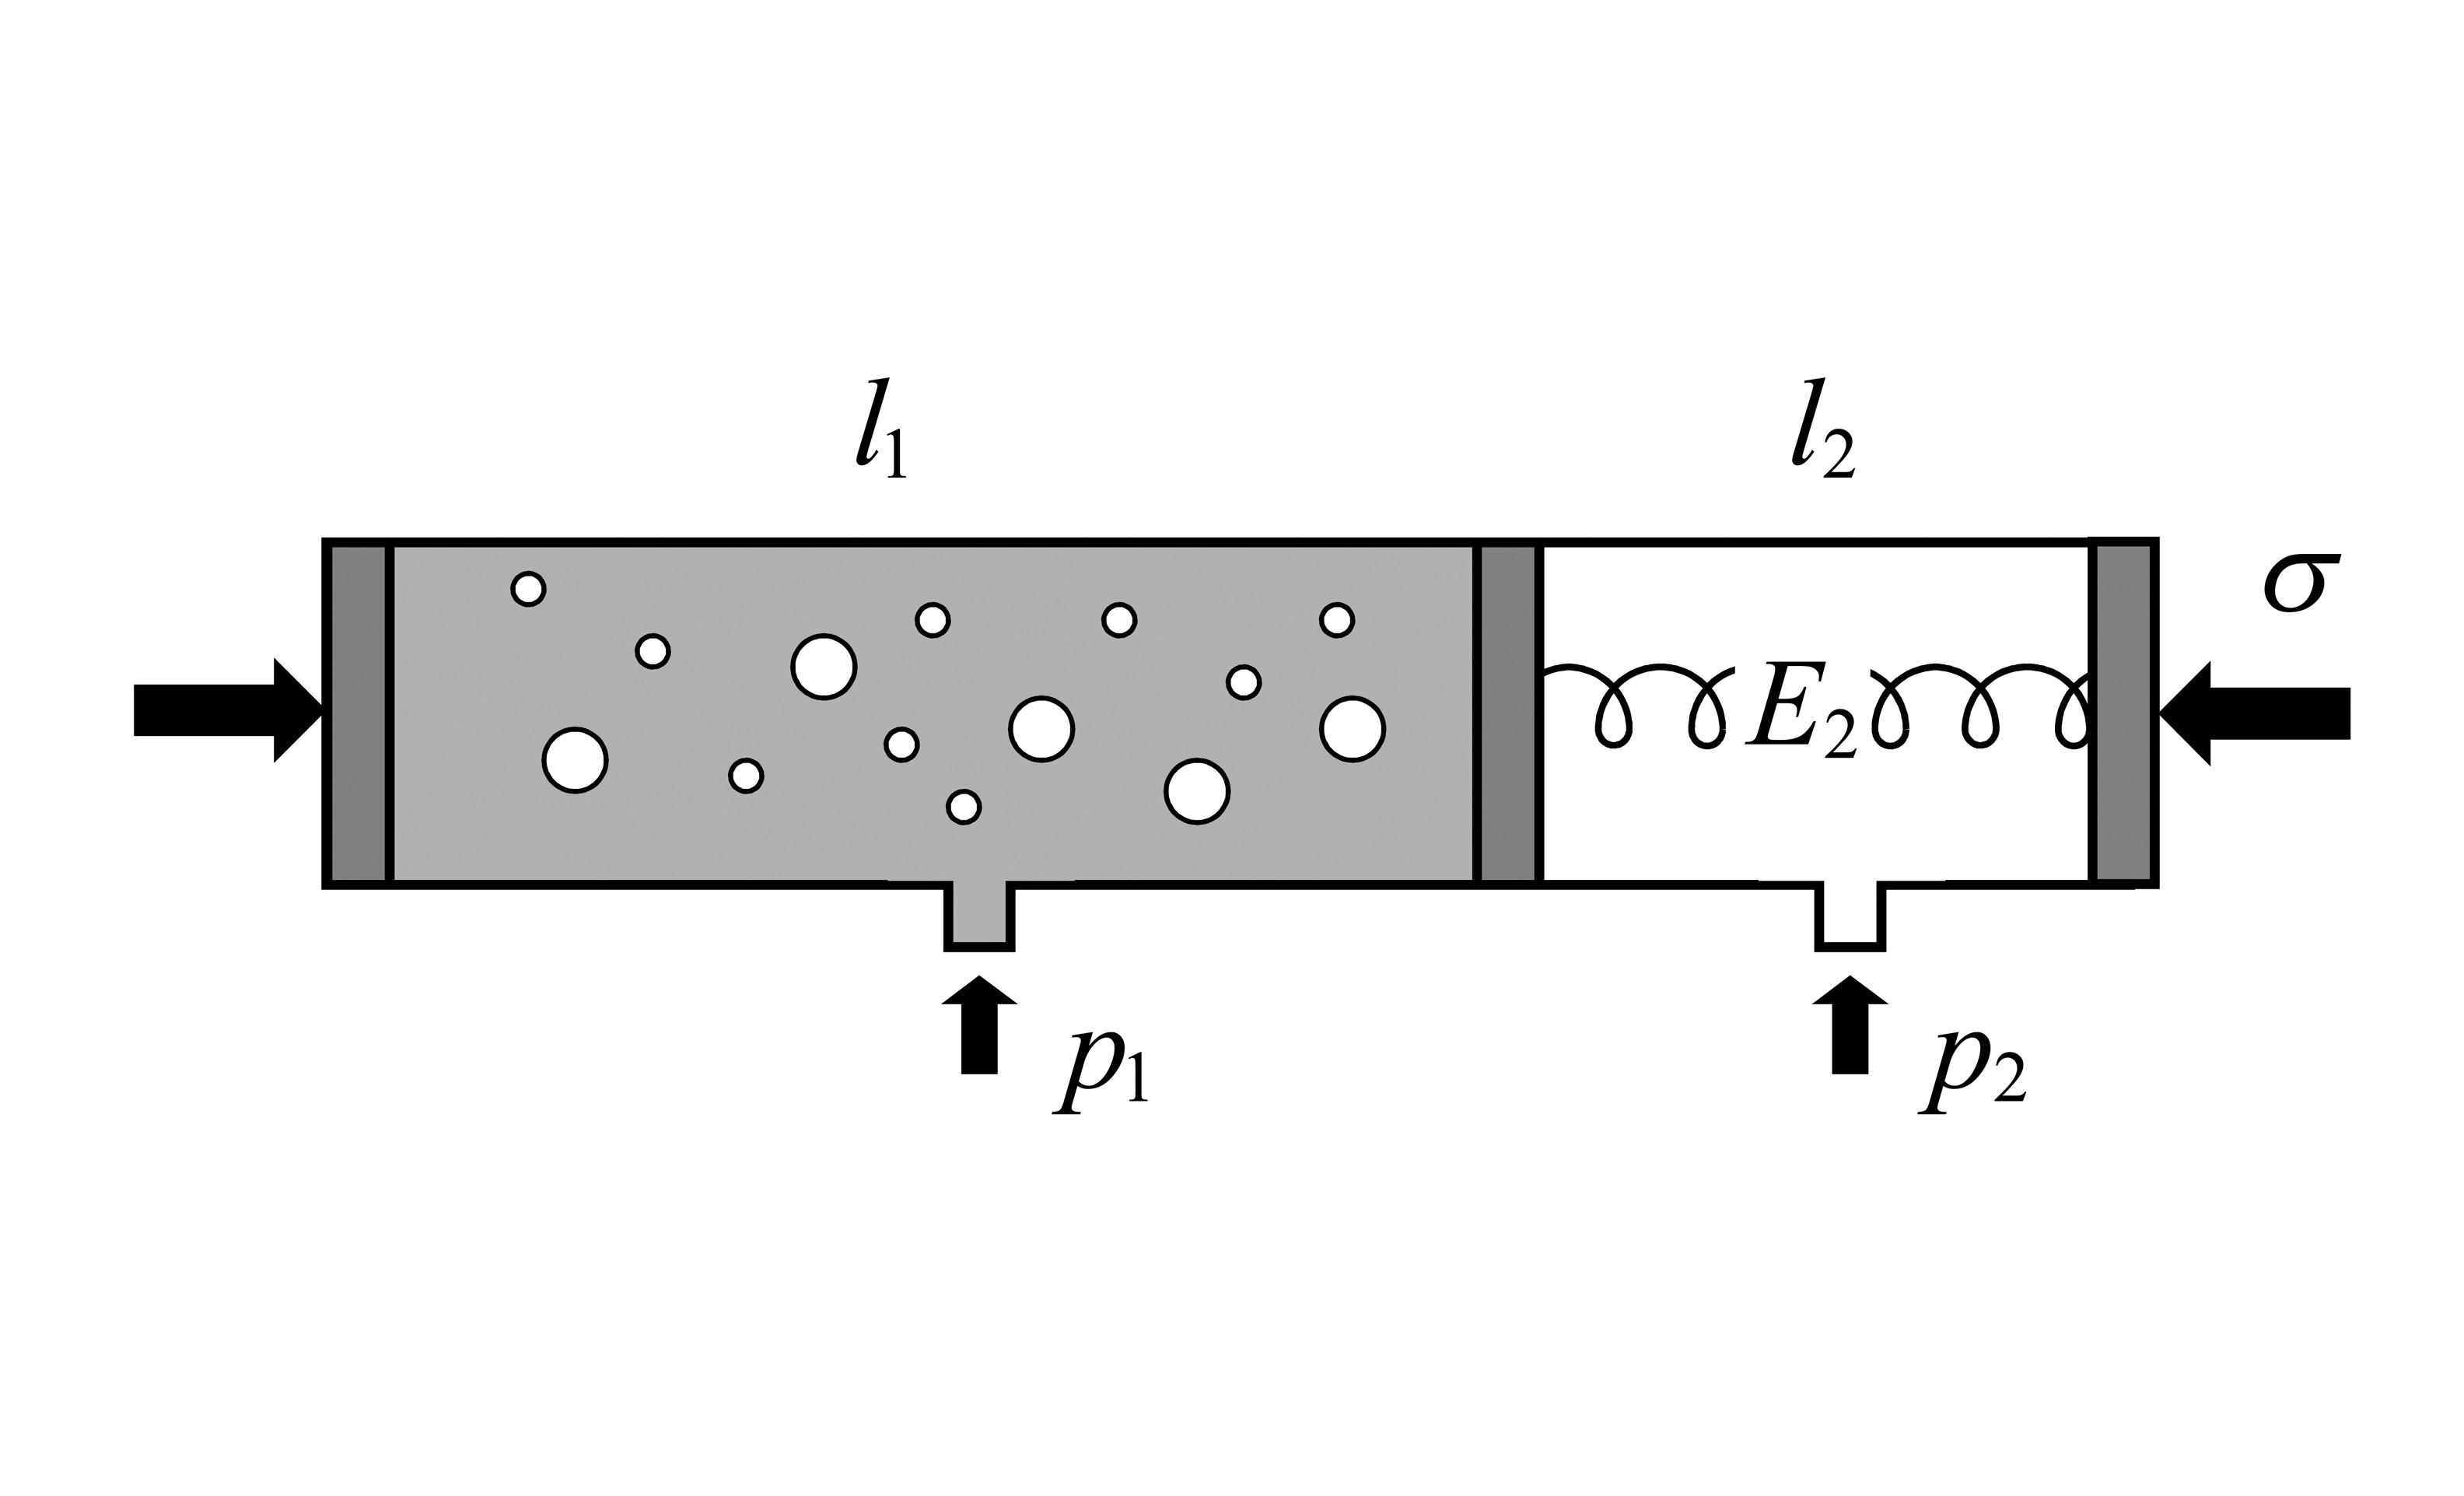
\includegraphics[width=0.6\linewidth]{coef2}}
        \hfill
    }
    % \legend{Упрощенная схема рассматриваемой среды (слева), упрощенная эквивалентная схема (справа).}
    \caption[Упрощенная схема рассматриваемой среды (слева), упрощенная эквивалентная схема (справа).]{Упрощенная схема рассматриваемой среды (слева), упрощенная эквивалентная схема (справа).}\label{fig:coef1}
\end{figure}

Запишем условия равновесия

\begin{equation}
  \label{eq:sigmaeq}
  \sigma = - \alpha_1 p_1 + E_1 \varepsilon_1 = - p_2 + E_2 \varepsilon_2,
\end{equation}
где $\sigma$~--- внешнее сжимающее напряжение, $\varepsilon_{\alpha} = \Delta l_{\alpha} / l_{\alpha}^0$~--- относительные удлинения элементов схемы.

Запишем общую деформацию системы $\varepsilon =  (\Delta l_1 + \Delta l_2) / (l_1^0 + l_2^0)$, как комбинацию относительных удлинений камер

\begin{equation}
  \label{eq:sigmaeq1}
  \varepsilon_{\Sigma} = \varepsilon_1 \xi_1 + \varepsilon_2 \xi_2.
\end{equation}
Выражая относительные удлинения из~\eqref{eq:sigmaeq}, с помощью~\eqref{eq:sigmaeq1} получим аналог закона Гука

\begin{equation}
  \label{eq:sigmaeq2}
  \sigma = E_{\Sigma} \varepsilon_{\Sigma} - \left( \alpha_1 \frac{E_{\Sigma}}{E_1} \xi_1 \right) p_1 + \left( \frac{E_{\Sigma}}{E_2} \xi_2 \right) p_2,
\end{equation}
где $E_{\Sigma} = (\xi_1 / E_1 + \xi_2 / E_2)^{-1}$~--- суммарный упругий модуль системы.

Сравнивая~\eqref{eq:sigmaeq2} с~\eqref{eq:linequationskelet1} в отсутствие поврежденности, приходим к выводу, что коэффициенты при давлениях $p_1$ и $p_2$ играют роль коэффициентов $b_1$ и $b_2$. Таким образом

\begin{equation}
  \label{eq:sigmaeq3}
  \frac{b_1}{b_2} = \frac{\alpha_1 \xi_1}{\xi_2} \frac{E_2}{E_1}.
\end{equation}
При стремлении объемной доли $\xi_2$ к нулю, суммарный упругий модуль системы $E_{\Sigma}$ стремится к $E_1$, а коэффициент $b_1$ стремится к коэффициенту Био матрицы $\alpha_1$. Пусть $\xi_2 \approx 0.01 \xi_1$, тогда при соотношении модулей $E_2/E_1 \approx 10^{-4} - 1$, отношение $b_1/b_2$ будет лежать в диапазоне $10^{-2} - 10^2$.

Модуль $E_2$ определяется, как $E_2 = S_n \Delta \lambda = S_n \xi_2 L$, где $S_n$~--- нормальная жесткость одиночной трещины, $\Delta \lambda$~--- ширина одиночной трещины, $L$~--- характерный размер блока~\autocite{kocharyan2016}.

Возьмем $S_n \approx 10^2$ ГПа/м, $L \approx 1$ м, $E_1 = 10$ ГПа, согласующиеся с данными из Таблиц~\ref{tab:coef1}, ~\ref{tab:coef2}, получим, что отношение упругих модулей будет равно $E_2/E_1 \approx 0.1$, тогда согласно~\eqref{eq:sigmaeq3} отношение $b_1/b_2 \approx 10$, а из~\eqref{eq:sigmaeq2} следует $b_1 = 0.9 \alpha_1$, $b_2 = 0.9 \alpha_1$.
Оценим модули $N_{\alpha}$ и $N_{12}$ с помощью предложенной упрощенной схемы. Учитывая, что деформация трещин $\varepsilon_2 = \Delta \phi_2/\phi_2$, деформация матрицы $\varepsilon_1 = \Delta \xi_1 / \xi_1 = \Delta \phi_1 / \phi_1 - \Delta n_1 / n_1$, при этом $\Delta n_1 = alpha_1 \varepsilon_1 + p_1 / \widetilde{N}$ из уравнений~\eqref{eq:sigmaeq} и~\eqref{eq:sigmaeq1} получим оценку

\begin{table} [htbp]%
    \centering
    \caption{}%
    \label{tab:coef1}% label всегда желательно идти после caption
    \renewcommand{\arraystretch}{1.5}%% Увеличение расстояния между рядами, для улучшения восприятия.
    \begin{SingleSpace}
        \begin{tabular}{@{}@{\extracolsep{20pt}}llll@{}} %Вертикальные полосы не используются принципиально, как и лишние горизонтальные (допускается по ГОСТ 2.105 пункт 4.4.5) % @{} позволяет прижиматься к краям
            \toprule     %%% верхняя линейка
            Величина & Значение & Материал \\
            \midrule %%% тонкий разделитель. Отделяет названия столбцов. Обязателен по ГОСТ 2.105 пункт 4.4.5
            $K_f$, ГПа          & 0.5-5~\autocite{craft1959petroleum}         & Нефть   \\
                                &    1.7~\autocite{abousleiman2005poromechanics}        &   \\
            \midrule
            $K_1$, ГПа          & 1.1~\autocite{abousleiman2005poromechanics}           & Сланцы (Gulf of Mexico)    \\
                                &    9.8~\autocite{abousleiman2007geomechanics}        &  Сланцы (Woodford shale) \\
            \midrule
            $\alpha_1$          & 0.96~\autocite{abousleiman2005poromechanics}          & Сланцы (Gulf of Mexico)   \\
            $\xi_2$             & 0.0001–0.01~\autocite{snow1968rock}  &   \\
            \midrule
            $S_n$, ГПа/м                  &    105–117~\autocite{ye2016fracture}      &  Сланцы (Barnett) \\
                                &    226~\autocite{ye2016fracture}       &  Сланцы (Mancos) \\
                                &    25–40~\autocite{ye2016fracture}        &  Сланцы (Pierre) \\
                                \midrule
            $L$, м                    &    0.2–30~\autocite{snow1968rock}        &   \\
            \midrule
            $E_1 = K_1 + \frac{4}{3}\mu $,                     &    2.1~\autocite{abousleiman2005poromechanics}        &  Сланцы (Gulf of Mexico) \\
            ГПа                    &    10–20         &  Сланцы (Woodford shale) \\
                                &    (анизотропия)~\autocite{abousleiman2007geomechanics}       &  \\
                                &    $5.1  \pm 0.5$~\autocite{eseme2007review}        &  Сланцы с высоким \\
                                &           &  содержанием органики \\
                                &    $16.6 \pm 2$~\autocite{eseme2007review}        &  Сланцы с низким \\
                                &           & содержанием органики  \\
                                \midrule
            $n_1$                  &    3.8\%~\autocite{abousleiman2007geomechanics}        &  Сланцы (Woodford shale) \\
                                &    14\%~\autocite{abousleiman2005poromechanics}       &  Сланцы (Gulf of Mexico) \\
                                \midrule
            $\widetilde{N}$, ГПа                    &    27.57~\autocite{abousleiman2005poromechanics}        & Сланцы (Gulf of Mexico)  \\

            \bottomrule %%% нижняя линейка
        \end{tabular}%
    \end{SingleSpace}
\end{table}

\begin{table} [htbp]%
    \centering
    \caption{}%
    \label{tab:coef2}% label всегда желательно идти после caption
    \renewcommand{\arraystretch}{1.5}%% Увеличение расстояния между рядами, для улучшения восприятия.
    \begin{SingleSpace}
        \begin{tabular}{@{}@{\extracolsep{20pt}}llll@{}} %Вертикальные полосы не используются принципиально, как и лишние горизонтальные (допускается по ГОСТ 2.105 пункт 4.4.5) % @{} позволяет прижиматься к краям
            \toprule     %%% верхняя линейка
            Величина & Значение & Материал \\
            \midrule %%% тонкий разделитель. Отделяет названия столбцов. Обязателен по ГОСТ 2.105 пункт 4.4.5
            $\nu \qquad \qquad \qquad$                    &    0.11–0.29       &  Сланцы (Woodford shale) \\
                                &    (анизотропия)~\autocite{abousleiman2007geomechanics}        &  \\
                                &    0.35~\autocite{eseme2007review}        & Сланцы с высоким  \\
                                &           &  содержанием органики \\
                                &    0.2~\autocite{eseme2007review}       &   Сланцы с низким \\
                                &           &  содержанием органики \\

            \bottomrule %%% нижняя линейка
        \end{tabular}%
    \end{SingleSpace}
\end{table}

\begin{equation}
  \label{eq:sigmaeq4}
  \frac{1}{N_1} = \frac{(\alpha_1 - b_1) (  + \alpha_1/n_1) \phi_1}{E_1} + \frac{\phi_1}{n_1 \widetilde{N}},
\end{equation}

\begin{equation}
  \label{eq:sigmaeq5}
  \frac{1}{N_2} = \frac{(1 - b_2) \phi_2}{E_2},
\end{equation}

\begin{equation}
  \label{eq:sigmaeq6}
  \frac{1}{N_{12}} = - \frac{b_1 \phi_2}{E_2}.
\end{equation}
Тогда для относительных величин справедливо

\begin{equation}
  \label{eq:sigmaeq7}
  \frac{N_2}{N_1} = \frac{1}{(1-b_2)} \left( (\alpha_1 - b_1) \left( 1 + \frac{\alpha_1}{n_1} \right) + \frac{E_1}{n_1 \widetilde{N}} \right) \frac{b_1}{b_2},
\end{equation}

\begin{equation}
  \label{eq:sigmaeq8}
  \frac{N_2}{N_{12}} = - \frac{b_1}{1 - b_2}.
\end{equation}

При $b_1/b_2 \approx 10$ и $\alpha_1 = 0.7$ из~\eqref{eq:sigmaeq8} получим оценку $N_2/N_{12} \approx 0.68$. Если дополнительно положить $n_1 = 0.1$ и $E_1/(n_1 \widetilde{N}) \approx 1$, тогда согласно соотношению~\eqref{eq:sigmaeq7} отношение $N_2/N_1 \approx 16.6$. Таким образом, абсолютные значения модулей  и  в рамках сделанных предположений имеют один порядок и более чем на порядок превышают модуль $N_1$. В последующих расчетах будем придерживаться полученных соотношений.

\section{Оценка параметров в модели поврежденности для матрицы}\label{sec:ch2/sec02}

В предложенную линейную модель поврежденности входит ряд коэффициентов. Оценим их, задавшись гипотезой о частном механизме разрушения матрицы. Обозначим коэффициенты, отвечающие за уменьшение упругой энергии матрицы $\alpha_M$, $\alpha_{JM}$, $\alpha_{pM}$ . В работах~\autocite{engelder1990natural, luo2002natural} указывается, что трещины автофлюидоразрыва развиваются преимущественно за счет нормального раскрытия. Принимая указанный механизм разрушения, положим, что в матрице содержится некоторое количество плоских круглых трещин (penny shaped) диаметром $l$, ориентация которых имеет изотропное распределение. Пренебрежем взаимодействием этих трещин, таким образом, уравнение~\eqref{eq:eq34} при $p_2 = 0$ соответствует условию начала развития одиночной трещины. В отличие от~\autocite{engelder1990natural} будем полагать, что стенки трещин непроницаемы для флюида, что правомерно в условиях сверхнизкой проницаемости.

В случае одноосного сжатия (рисунок~\ref{fig:coef2-1}) под действием внутреннего давления первой раскроется трещина, ориентированная перпендикулярно максимальному сжимающему напряжению $\sigma_V < 0$. Это произойдет при внутреннем давлении $p_{ini}$, равном~\autocite{engelder1990natural}

\begin{figure}[ht]
    \centerfloat{
        \hfill
        \subcaptionbox[List-of-Figures entry]{\label{fig:coef2-1}}{%
            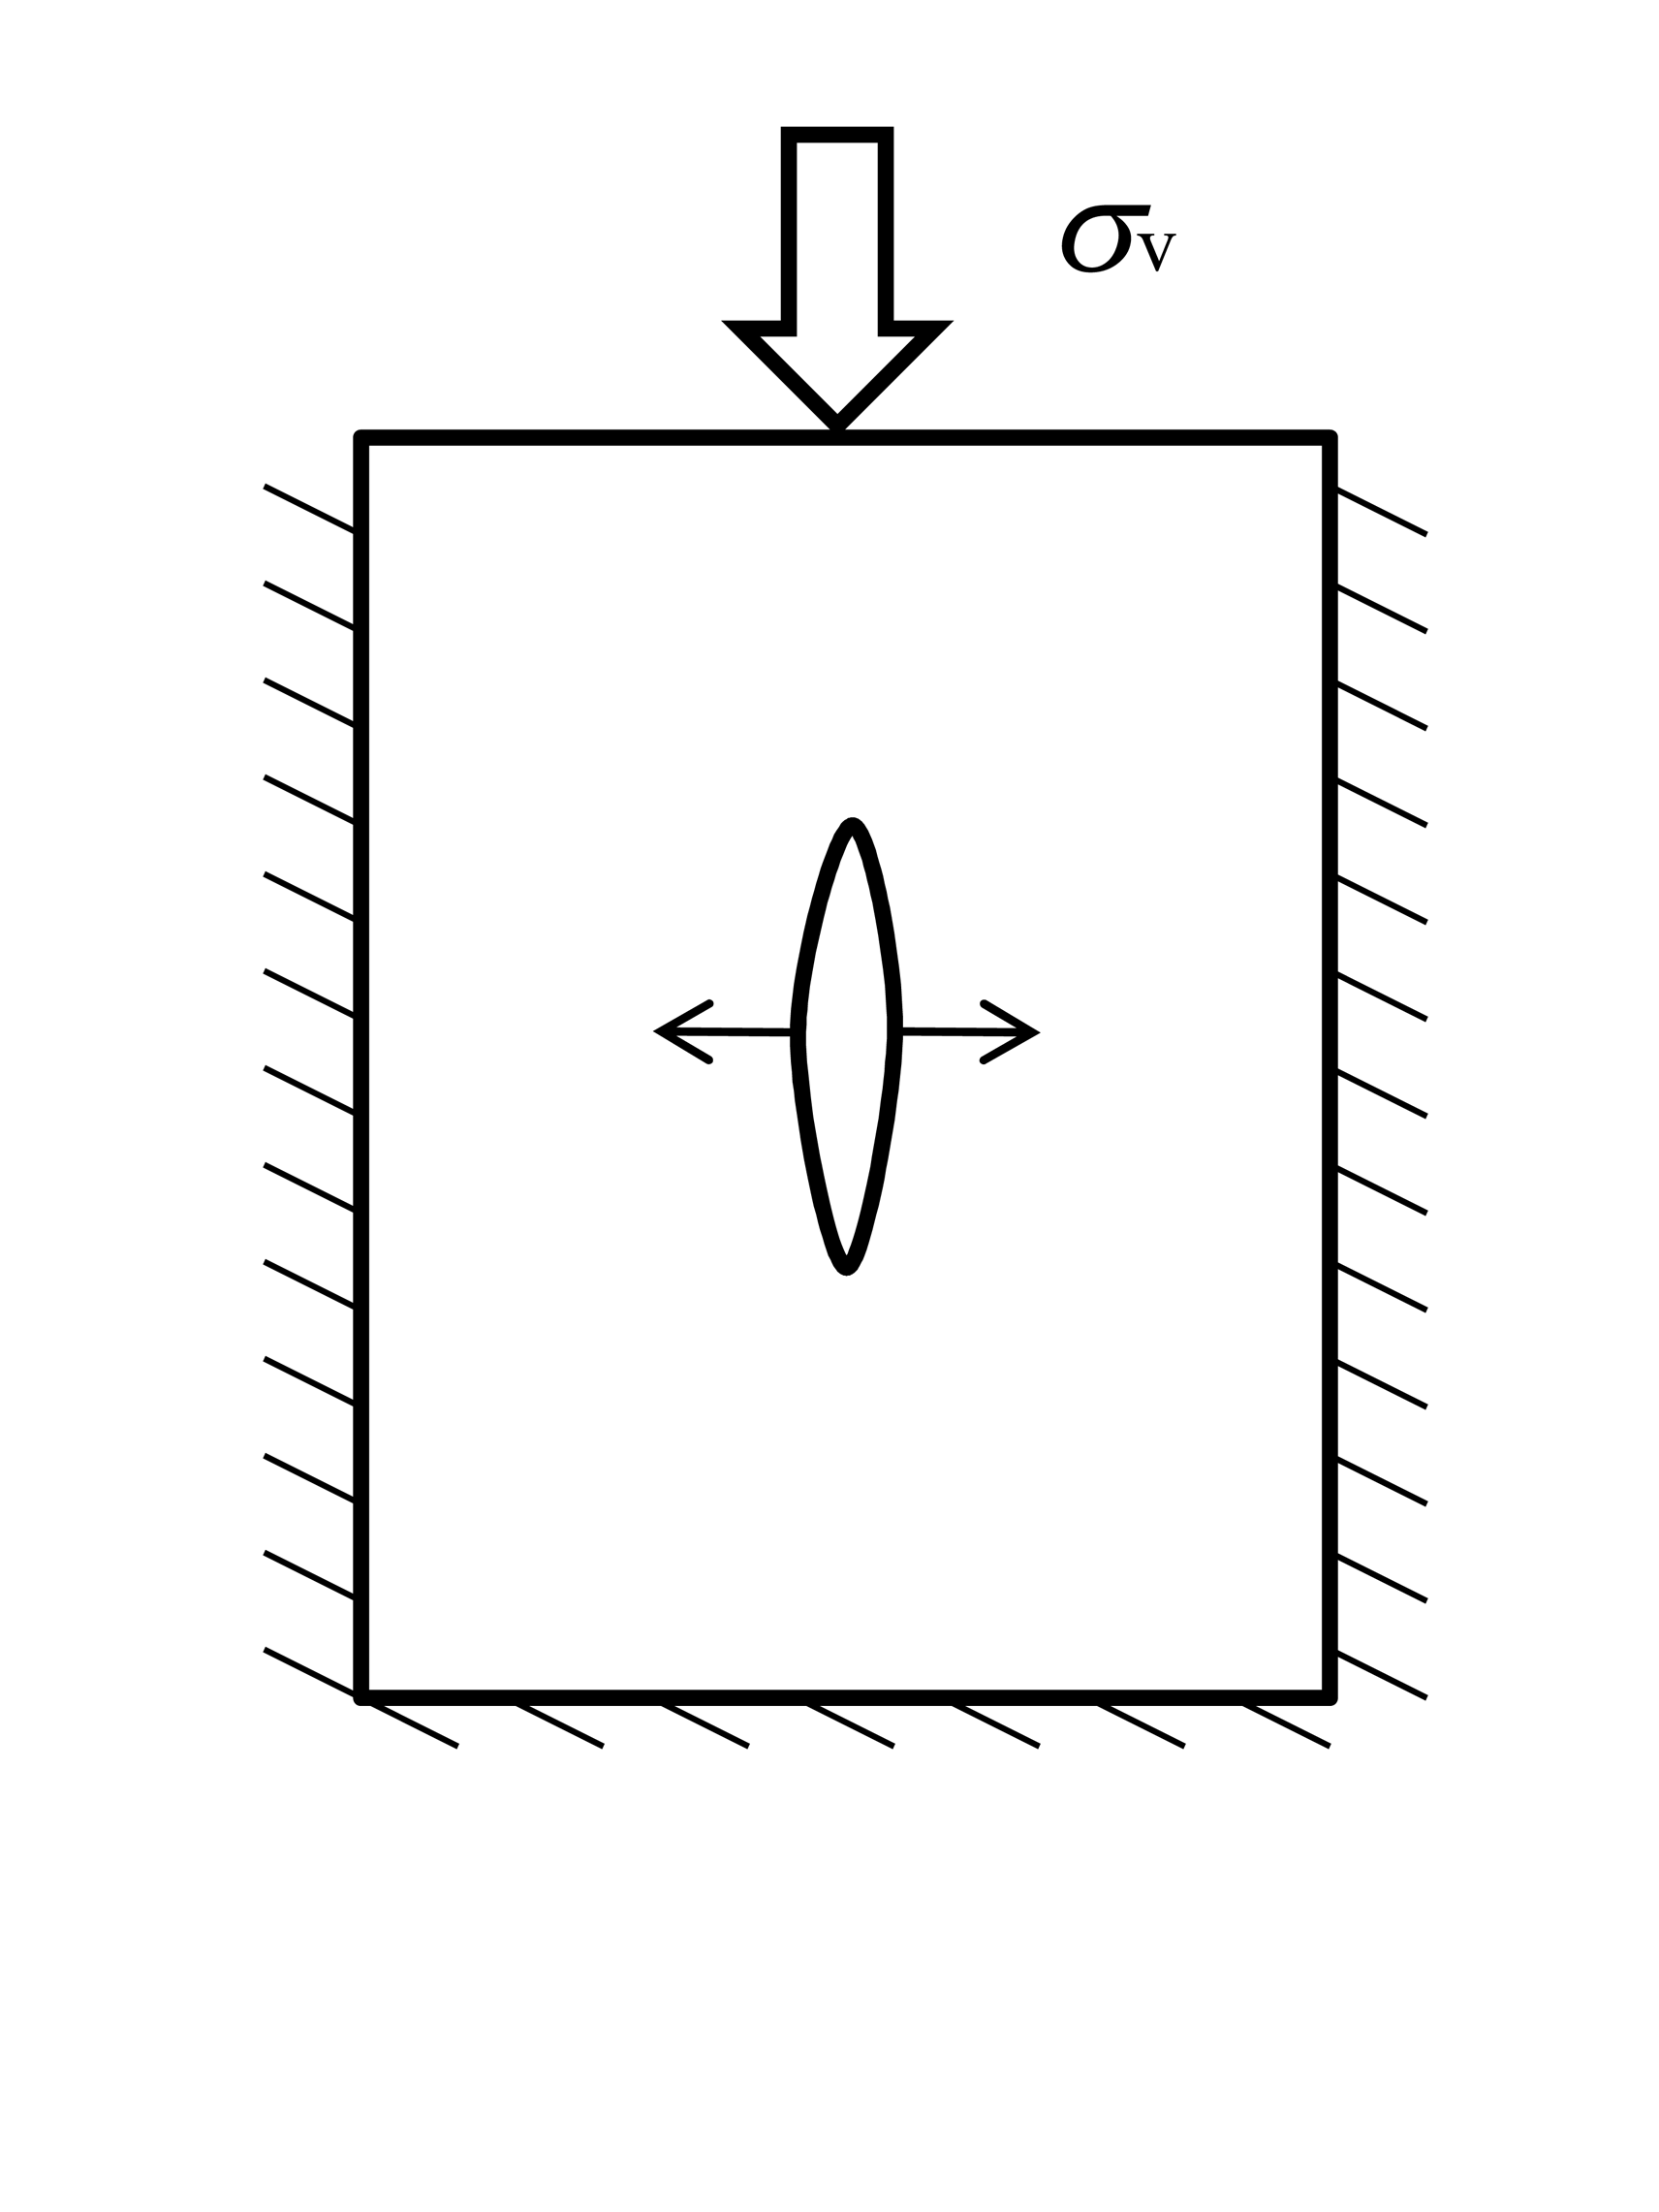
\includegraphics[width=0.4\linewidth]{coef3}}
        \hfill
        \subcaptionbox{\label{fig:coef2-2}}{%
            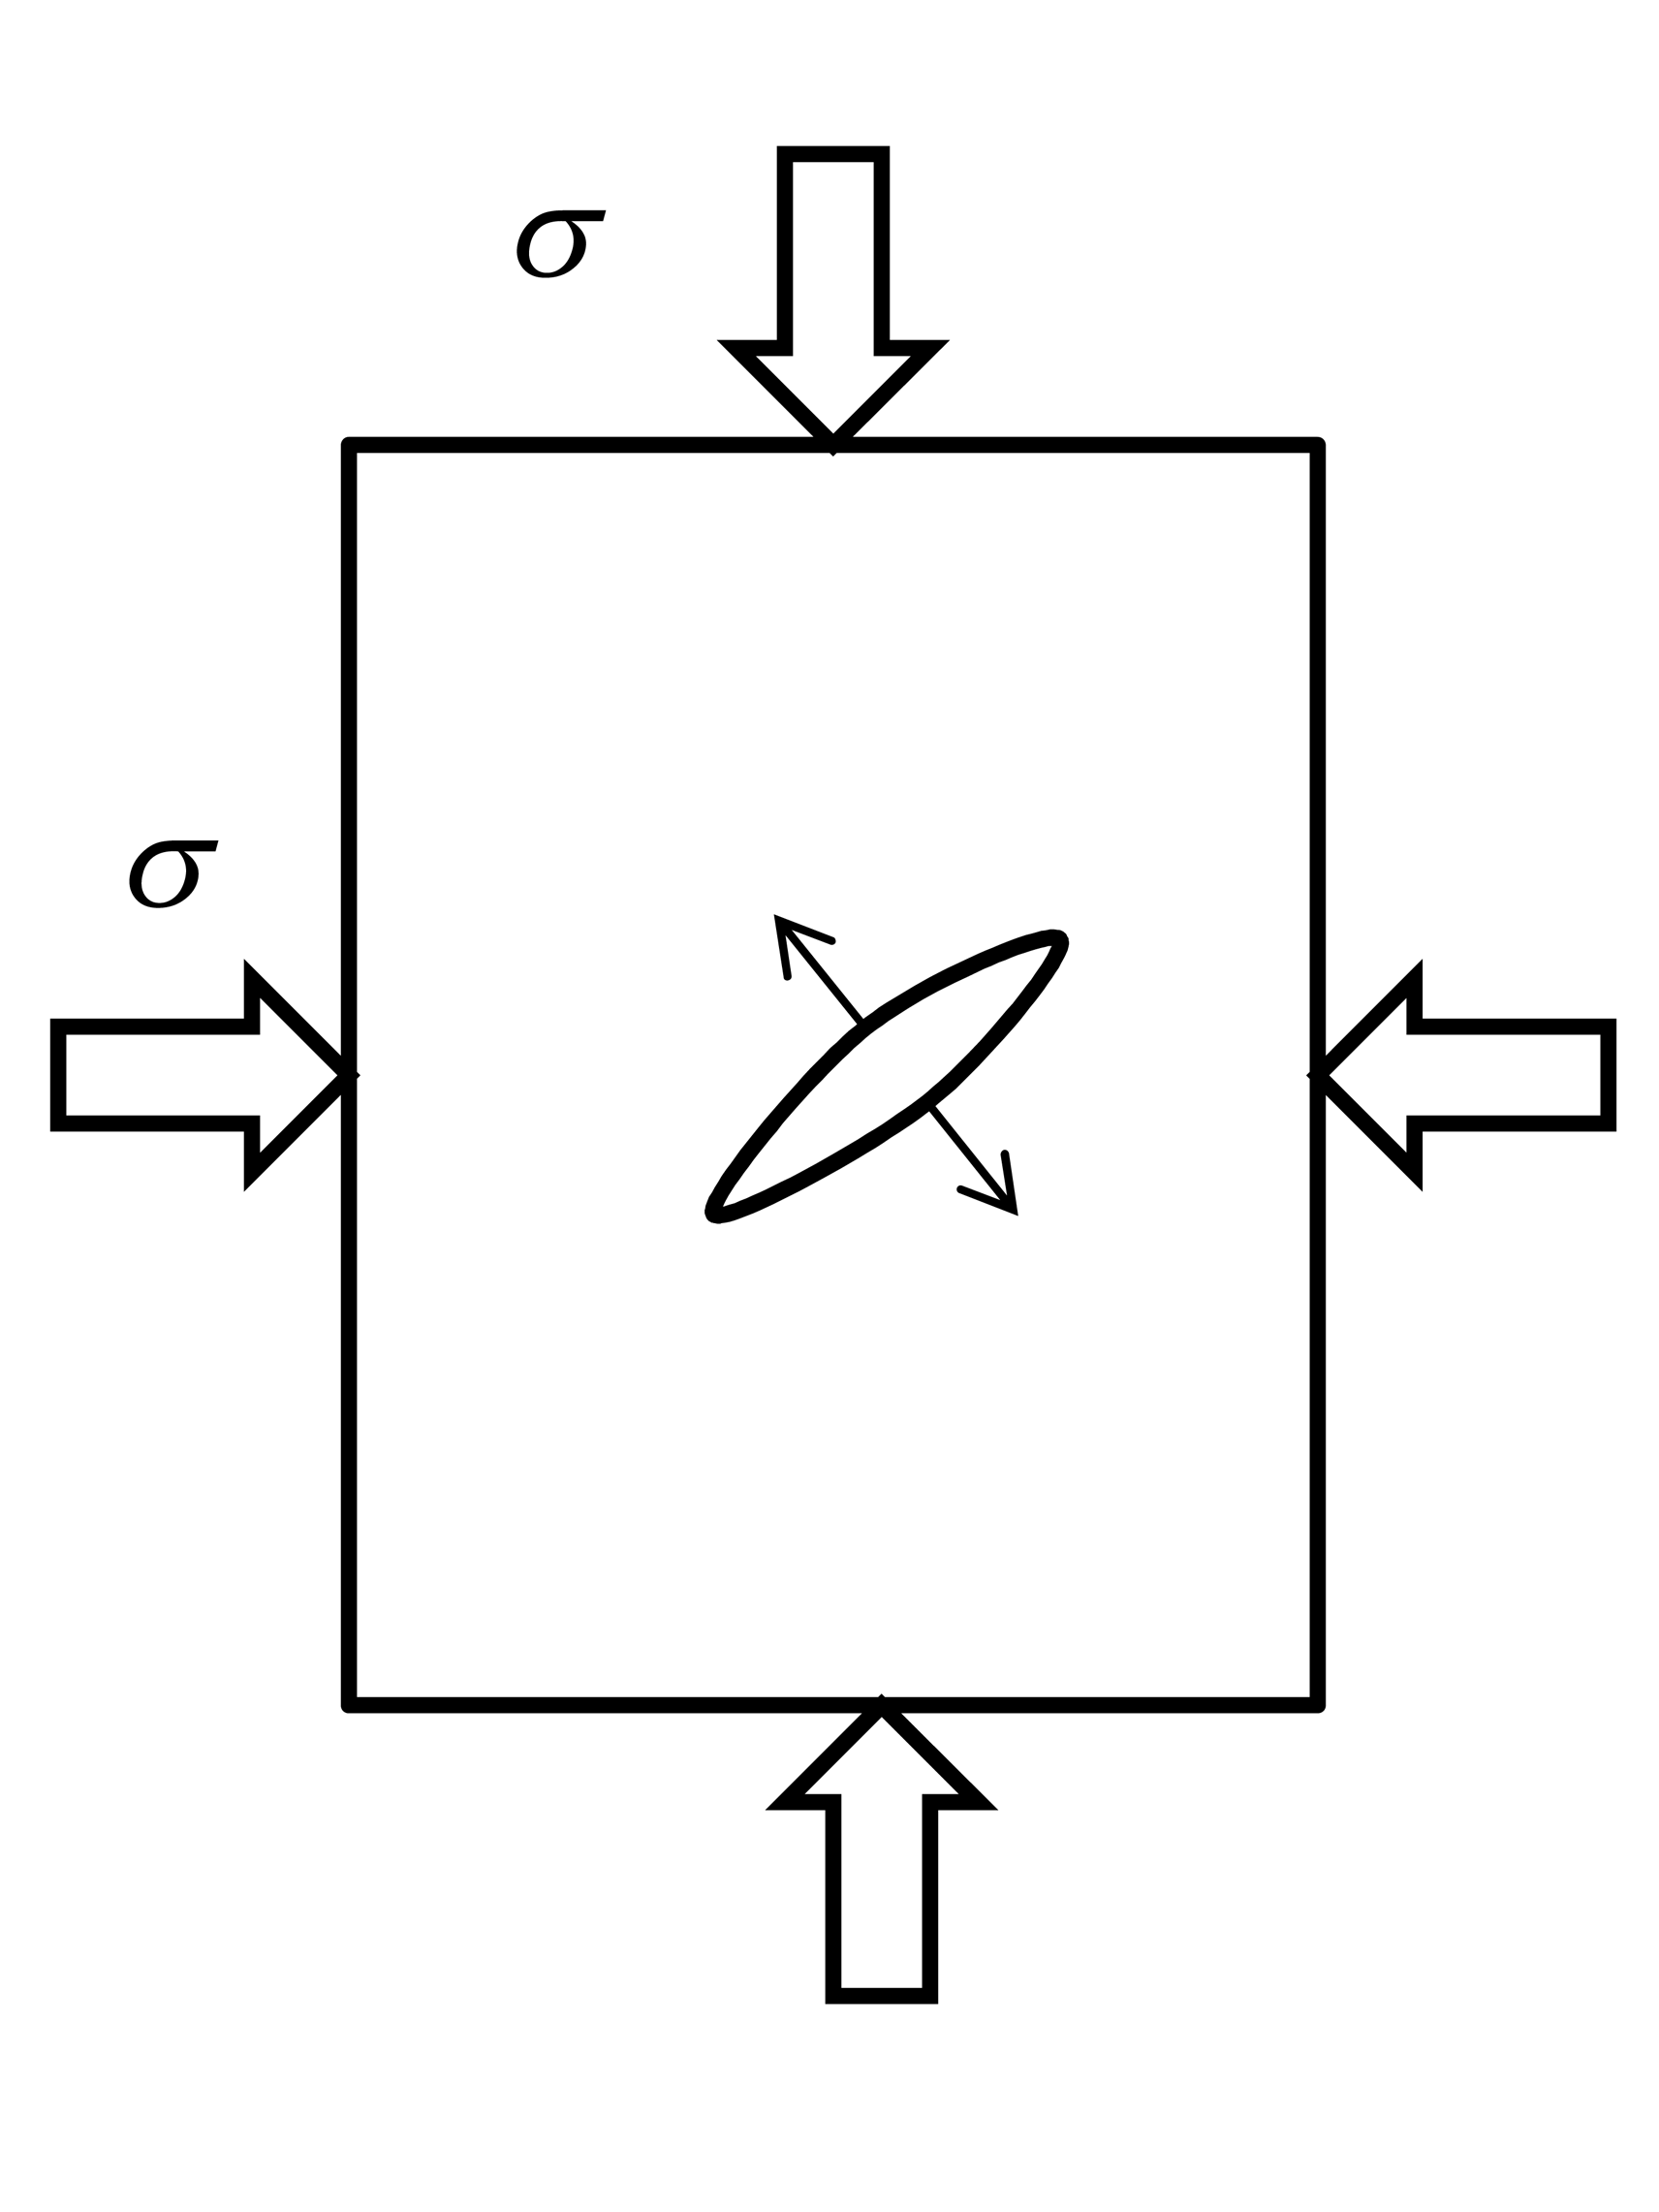
\includegraphics[width=0.4\linewidth]{coef4}}
        \hfill
    }
    % \legend{Одноосное сжатие (слева); гидростатическое сжатие (справа).}
    \caption[Одноосное сжатие (слева); гидростатическое сжатие (справа).]{Одноосное сжатие (слева); гидростатическое сжатие (справа).}\label{fig:coef2}
\end{figure}

\begin{equation}
  \label{eq:omegaeq1}
  p_{ini} = \frac{K_{IC}}{1.13 \sqrt{l}} - \frac{\nu}{1 - \nu }\sigma_V,
\end{equation}
где $\nu$~--- коэффициент Пуассона, $K_{IC}$~--- критический коэффициент интенсивности напряжений при нормальном раскрытии одиночной трещины.

В случае всестороннего сжатия (рисунок~\ref{fig:coef2-2}) уравнение для критического давления будет иметь вид

\begin{equation}
  \label{eq:omegaeq2}
  p_{ini} = \frac{K_{IC}}{1.13 \sqrt{l}} - \sigma.
\end{equation}

Сравнивая~\eqref{eq:linequationskelet5} с~\eqref{eq:linequationskelet2}, получим оценки

\begin{equation}
  \label{eq:omegaeq3}
  \frac{\alpha_{JM}}{\alpha_{PM}} = K,
\end{equation}

\begin{equation}
  \label{eq:omegaeq4}
  \frac{\gamma}{\alpha_{PM}} = \frac{K_{IC}}{1.13 \sqrt{l}}.
\end{equation}

Аналогично рассматривая трещину в условиях одноосного сжатия (в этом случае $J = -\sqrt{2/3}I_1$), получим

\begin{equation}
  \label{eq:omegaeq4}
  \frac{\alpha_{JM}}{\alpha_{M}} = \frac{3 - 7 \nu +2 \nu^2}{\sqrt{6}(1-\nu)^2}.
\end{equation}

В работе~\autocite{grytsenko2010numerical} с помощью численных расчетов методом сингулярных интегральных уравнений было показано, что в случае ансамбля из большого числа одинаковых трещин, находящихся на расстояниях больше либо порядка их длины, критический коэффициент интенсивности напряжений зависит от взаимного расположения трещин, однако отличается от $K_{IC}$ не более чем на $30\%$ (в меньшую сторону).

Параметр $\beta$ в расчетах подбирался таким, чтобы выполнялось неравенство $\alpha_{M}^2 /\beta < K$.

\section{Условие разрушения среды с двойной пористостью}\label{sec:ch2/sec03}

Обратимся теперь к среде с двойной пористостью. Воспользуемся одномерной моделью. Пусть условие начала поврежденности в матрице имеет вид:

\begin{equation}
  \label{eq:destroy1}
  \alpha_M \varepsilon_1 + \alpha_{pM} p_1 - \gamma = 0.
\end{equation}
Требуется переформулировать его в терминах полной деформации $\varepsilon_{\Sigma}$. Исключим  из условия~\eqref{eq:destroy1} с помощью~\eqref{eq:sigmaeq}и~\eqref{eq:sigmaeq1}. В итоге получим

\begin{equation}
  \label{eq:destroy1}
  \frac{\alpha_M }{\xi_1} (1 - b_2) \varepsilon_{\Sigma} + \alpha_M(a_1 p_1 - a_2 p_2) - \alpha_{pM}p_1- \gamma = 0,
\end{equation}
где $a_1=\frac{\xi_2}{\xi_1}\frac{b_1}{E_2}, a_2 = \frac{b_2}{E_1}$.

Сравнивая полученное выражение с~\eqref{eq:eq34}, получим, что

\begin{equation}
  \label{eq:destroy2}
  \alpha = \frac{\alpha_M}{\xi_1} (1 - b_2),
\end{equation}

\begin{equation}
  \label{eq:destroy3}
  \alpha_{p1} = \alpha_{M}a_1+ \alpha_{pM} \geq 0,
\end{equation}

\begin{equation}
  \label{eq:destroy4}
  \alpha_{p2} = - \alpha_{M}a_2 \leq 0.
\end{equation}

Используя ранее сделанные оценки $b_1/b_2 \approx 10$, $E_2/E_1 \approx 0.1$, $\xi_2 \approx 0.01 \xi_1$, получим $a_1 \approx a_2$, $\alpha \approx \alpha_M$. Далее, используя оценку  (одномерный аналог~\eqref{eq:omegaeq3}), получим соотношение между коэффициентами $\alpha_{p_1}$ и $\alpha_{p2}$:

\begin{equation}
  \label{eq:destroy4}
  \alpha_{p2} \approx \alpha_{p_1} b_2 \leq 0.
\end{equation}


% \begin{figure}[ht]
%   \centerfloat{
%     \includegraphics[scale=0.27]{latex}
%   }
%   \caption{TeX.}\label{fig:latex}
% \end{figure}
%
% Для выравнивания изображения по-центру используется команда \verb+\centerfloat+, которая является во
% многом улучшенной версией встроенной команды \verb+\centering+.
%
% \section{Длинное название параграфа, в котором мы узнаём как сделать две картинки с~общим номером и названием}\label{sec:ch2/sect2}
%
% А это две картинки под общим номером и названием:
% \begin{figure}[ht]
%   \begin{minipage}[b][][b]{0.49\linewidth}\centering
%     \includegraphics[width=0.5\linewidth]{knuth1} \\ а)
%   \end{minipage}
%   \hfill
%   \begin{minipage}[b][][b]{0.49\linewidth}\centering
%     \includegraphics[width=0.5\linewidth]{knuth2} \\ б)
%   \end{minipage}
%   \caption{Очень длинная подпись к изображению,
%       на котором представлены две фотографии Дональда Кнута}
%   \label{fig:knuth}
% \end{figure}
%
% Те~же~две картинки под~общим номером и~названием,
% но с автоматизированной нумерацией подрисунков:
% \begin{figure}[ht]
%     \centerfloat{
%         \hfill
%         \subcaptionbox[List-of-Figures entry]{Первый подрисунок\label{fig:knuth_2-1}}{%
%             \includegraphics[width=0.25\linewidth]{knuth1}}
%         \hfill
%         \subcaptionbox{\label{fig:knuth_2-2}}{%
%             \includegraphics[width=0.25\linewidth]{knuth2}}
%         \hfill
%         \subcaptionbox{Третий подрисунок, подпись к которому
%         не~помещается на~одной строке}{%
%             \includegraphics[width=0.3\linewidth]{example-image-c}}
%         \hfill
%     }
%     \legend{Подрисуночный текст, описывающий обозначения, например. Согласно
%     ГОСТ 2.105, пункт 4.3.1, располагается перед наименованием рисунка.}
%     \caption[Этот текст попадает в названия рисунков в списке рисунков]{Очень
%     длинная подпись к второму изображению, на~котором представлены две
%     фотографии Дональда Кнута}\label{fig:knuth_2}
% \end{figure}
%
% На рисунке~\ref{fig:knuth_2-1} показан Дональд Кнут без головного убора.
% На рисунке~\ref{fig:knuth_2}\subcaptionref*{fig:knuth_2-2}
% показан Дональд Кнут в головном уборе.
%
% Возможно вставлять векторные картинки, рассчитываемые \LaTeX\ <<на~лету>>
% с~их~предварительной компиляцией. Надписи в таких рисунках будут выполнены
% тем же~шрифтом, который указан для документа в целом.
% На~рисунке~\ref{fig:tikz_example} на~странице~\pageref{fig:tikz_example}
% представлен пример схемы, рассчитываемой пакетом \verb|tikz| <<на~лету>>.
% Для ускорения компиляции, подобные рисунки могут быть <<кешированы>>, что
% определяется настройками в~\verb|common/setup.tex|.
% Причём имя предкомпилированного
% файла и~папка расположения таких файлов могут быть отдельно заданы,
% что удобно, если не~для подготовки диссертации,
% то~для подготовки научных публикаций.
% \begin{figure}[ht]
%     \centerfloat{
%         \ifdefmacro{\tikzsetnextfilename}{\tikzsetnextfilename{tikz_example_compiled}}{}% присваиваемое предкомпилированному pdf имя файла (не обязательно)
%         \input{Dissertation/images/tikz_scheme.tikz}
%
%     }
%     \legend{}
%     \caption[Пример \texttt{tikz} схемы]{Пример рисунка, рассчитываемого
%         \texttt{tikz}, который может быть предкомпилирован}\label{fig:tikz_example}
% \end{figure}
%
% Множество программ имеют либо встроенную возможность экспортировать векторную
% графику кодом \verb|tikz|, либо соответствующий пакет расширения.
% Например, в GeoGebra есть встроенный экспорт,
% для Inkscape есть пакет svg2tikz,
% для Python есть пакет matplotlib2tikz,
% для R есть пакет tikzdevice.
%
% \section{Пример вёрстки списков}\label{sec:ch2/sec3}
%
% \noindent Нумерованный список:
% \begin{enumerate}
%   \item Первый пункт.
%   \item Второй пункт.
%   \item Третий пункт.
% \end{enumerate}
%
% \noindent Маркированный список:
% \begin{itemize}
%   \item Первый пункт.
%   \item Второй пункт.
%   \item Третий пункт.
% \end{itemize}
%
% \noindent Вложенные списки:
% \begin{itemize}
%   \item Имеется маркированный список.
%   \begin{enumerate}
%     \item В нём лежит нумерованный список,
%     \item в котором
%     \begin{itemize}
%       \item лежит ещё один маркированный список.
%     \end{itemize}
%   \end{enumerate}
% \end{itemize}
%
% \noindent Нумерованные вложенные списки:
% \begin{enumerate}
%   \item Первый пункт.
%   \item Второй пункт.
%   \item Вообще, по ГОСТ 2.105 первый уровень нумерации
%   (при необходимости ссылки в тексте документа на одно из перечислений)
%   идёт буквами русского или латинского алфавитов,
%   а второй "--- цифрами со~скобками.
%   Здесь отходим от ГОСТ.
%     \begin{enumerate}
%       \item в нём лежит нумерованный список,
%       \item в котором
%         \begin{enumerate}
%           \item ещё один нумерованный список,
%           \item третий уровень нумерации не нормирован ГОСТ 2.105;
%           \item обращаем внимание на строчность букв,
%           \item в этом списке
%           \begin{itemize}
%             \item лежит ещё один маркированный список.
%           \end{itemize}
%         \end{enumerate}
%
%     \end{enumerate}
%
%   \item Четвёртый пункт.
% \end{enumerate}
%
% \section{Традиции русского набора}
%
% Много полезных советов приведено в материале
% <<\href{http://www.dropbox.com/s/x4hajy4pkw3wdql/wholesome-typesetting.pdf?dl=1\&pv=1}{Краткий курс благородного набора}>> (автор А.\:В.~Костырка).
% Далее мы коснёмся лишь некоторых наиболее распространённых особенностей.
%
% \subsection{Пробелы}
%
% В~русском наборе принято:
% \begin{itemize}
%     \item единицы измерения, знак процента отделять пробелами от~числа:
%         10~кВт, 15~\% (согласно ГОСТ 8.417, раздел 8);
%     \item \(\tg 20\text{\textdegree}\), но: 20~{\textdegree}C
%         (согласно ГОСТ 8.417, раздел 8);
%     \item знак номера, параграфа отделять от~числа: №~5, \S~8;
%     \item стандартные сокращения: т.\:е., и~т.\:д., и~т.\:п.;
%     \item неразрывные пробелы в~предложениях.
% \end{itemize}
%
% \subsection{Математические знаки и символы}
%
% Русская традиция начертания греческих букв и некоторых математических
% функций отличается от~западной. Это исправляется серией
% \verb|\renewcommand|.
% \begin{itemize}
% %Все \original... команды заранее, ради этого примера, определены в Dissertation\userstyles.tex
%     \item[До:] \( \originalepsilon \originalge \originalphi\),
%     \(\originalphi \originalleq \originalepsilon\),
%     \(\originalkappa \in \originalemptyset\),
%     \(\originaltan\),
%     \(\originalcot\),
%     \(\originalcsc\).
%     \item[После:] \( \epsilon \ge \phi\),
%     \(\phi \leq \epsilon\),
%     \(\kappa \in \emptyset\),
%     \(\tan\),
%     \(\cot\),
%     \(\csc\).
% \end{itemize}
%
% Кроме того, принято набирать греческие буквы вертикальными, что
% решается подключением пакета \verb|upgreek| (см. закомментированный
% блок в~\verb|userpackages.tex|) и~аналогичным переопределением в
% преамбуле (см.~закомментированный блок в~\verb|userstyles.tex|). В
% этом шаблоне такие переопределения уже включены.
%
% Знаки математических операций принято переносить. Пример переноса
% в~формуле~\eqref{eq:equation3}.
%
% \subsection{Кавычки}
% В английском языке приняты одинарные и двойные кавычки в~виде ‘...’ и~“...”.
% В России приняты французские («...») и~немецкие („...“) кавычки (они называются
% «ёлочки» и~«лапки», соответственно). ,,Лапки`` обычно используются внутри
% <<ёлочек>>, например, <<... наш гордый ,,Варяг``...>>.
%
% Французкие левые и правые кавычки набираются
% как лигатуры \verb|<<| и~\verb|>>|, а~немецкие левые
% и правые кавычки набираются как лигатуры \verb|,,| и~\verb|‘‘| (\verb|``|).
%
% Вместо лигатур или команд с~активным символом "\ можно использовать команды
% \verb|\glqq| и \verb|\grqq| для набора немецких кавычек и команды \verb|\flqq|
% и~\verb|\frqq| для набора французских кавычек. Они определены в пакете
% \verb|babel|.
%
% \subsection{Тире}
% %  babel+pdflatex по умолчанию, в polyglossia надо включать опцией (и перекомпилировать с удалением временных файлов)
% Команда \verb|"---| используется для печати тире в тексте. Оно несколько короче
% английского длинного тире. Кроме того, команда задаёт небольшую жёсткую отбивку
% от слова, стоящего перед тире. При этом, само тире не~отрывается от~слова.
% После тире следует такая же отбивка от текста, как и~перед тире. При наборе
% текста между словом и командой, за которым она следует, должен стоять пробел.
%
% В составных словах, таких, как <<Закон Менделеева"--~Клапейрона>>, для печати
% тире надо использовать команду \verb|"--~|. Она ставит более короткое,
% по~сравнению с~английским, тире и позволяет делать переносы во втором слове.
% При~наборе текста команда \verb|"--~| не отделяется пробелом от слова,
% за~которым она следует (\verb|Менделеева"--~|). Следующее за командой слово
% может быть  отделено от~неё пробелом или перенесено на другую строку.
%
% Если прямая речь начинается с~абзаца, то перед началом её печатается тире
% командой \verb|"--*|. Она печатает русское тире и жёсткую отбивку нужной
% величины перед текстом.
%
% \subsection{Дефисы и переносы слов}
% %  babel+pdflatex по умолчанию, в polyglossia надо включать опцией (и перекомпилировать с удалением временных файлов)
% Для печати дефиса в~составных словах введены две команды. Команда~\verb|"~|
% печатает дефис и~запрещает делать переносы в~самих словах, а~команда \verb|"=|
% печатает дефис, оставляя \TeX ’у право делать переносы в~самих словах.
%
% В отличие от команды \verb|\-|, команда \verb|"-| задаёт место в~слове, где
% можно делать перенос, не~запрещая переносы и~в~других местах слова.
%
% Команда \verb|""| задаёт место в~слове, где можно делать перенос, причём дефис
% при~переносе в~этом месте не~ставится.
%
% Команда \verb|",| вставляет небольшой пробел после инициалов с~правом переноса
% в~фамилии.
%
% \section{Текст из панграмм и формул}
%
% Любя, съешь щипцы, "--- вздохнёт мэр, "--- кайф жгуч. Шеф взъярён тчк щипцы
% с~эхом гудбай Жюль. Эй, жлоб! Где туз? Прячь юных съёмщиц в~шкаф. Экс-граф?
% Плюш изъят. Бьём чуждый цен хвощ! Эх, чужак! Общий съём цен шляп (юфть) "---
% вдрызг! Любя, съешь щипцы, "--- вздохнёт мэр, "--- кайф жгуч. Шеф взъярён тчк
% щипцы с~эхом гудбай Жюль. Эй, жлоб! Где туз? Прячь юных съёмщиц в~шкаф.
% Экс-граф? Плюш изъят. Бьём чуждый цен хвощ! Эх, чужак! Общий съём цен шляп
% (юфть) "--- вдрызг! Любя, съешь щипцы, "--- вздохнёт мэр, "--- кайф жгуч. Шеф
% взъярён тчк щипцы с~эхом гудбай Жюль. Эй, жлоб! Где туз? Прячь юных съёмщиц
% в~шкаф. Экс-граф? Плюш изъят. Бьём чуждый цен хвощ! Эх, чужак! Общий съём цен
% шляп (юфть) "--- вдрызг! Любя, съешь щипцы, "--- вздохнёт мэр, "--- кайф жгуч.
% Шеф взъярён тчк щипцы с~эхом гудбай Жюль. Эй, жлоб! Где туз? Прячь юных съёмщиц
% в~шкаф. Экс-граф? Плюш изъят. Бьём чуждый цен хвощ! Эх, чужак! Общий съём цен
% шляп (юфть) "--- вдрызг! Любя, съешь щипцы, "--- вздохнёт мэр, "--- кайф жгуч.
% Шеф взъярён тчк щипцы с~эхом гудбай Жюль. Эй, жлоб! Где туз? Прячь юных съёмщиц
% в~шкаф. Экс-граф? Плюш изъят. Бьём чуждый цен хвощ! Эх, чужак! Общий съём цен
% шляп (юфть) "--- вдрызг! Любя, съешь щипцы, "--- вздохнёт мэр, "--- кайф жгуч.
% Шеф взъярён тчк щипцы с~эхом гудбай Жюль. Эй, жлоб! Где туз? Прячь юных съёмщиц
% в~шкаф. Экс-граф? Плюш изъят. Бьём чуждый цен хвощ! Эх, чужак! Общий съём цен
% шляп (юфть) "--- вдрызг! Любя, съешь щипцы, "--- вздохнёт мэр, "--- кайф жгуч.
% Шеф взъярён тчк щипцы с~эхом гудбай Жюль. Эй, жлоб! Где туз? Прячь юных съёмщиц
% в~шкаф. Экс-граф? Плюш изъят. Бьём чуждый цен хвощ! Эх, чужак! Общий съём цен
% шляп (юфть) "--- вдрызг! Любя, съешь щипцы, "--- вздохнёт мэр, "--- кайф жгуч.
% Шеф взъярён тчк щипцы с~эхом гудбай Жюль. Эй, жлоб! Где туз? Прячь юных съёмщиц
% в~шкаф. Экс-граф? Плюш изъят. Бьём чуждый цен хвощ! Эх, чужак! Общий съём цен
% шляп (юфть) "--- вдрызг! Любя, съешь щипцы, "--- вздохнёт мэр, "--- кайф жгуч.
% Шеф взъярён тчк щипцы с~эхом гудбай Жюль. Эй, жлоб! Где туз? Прячь юных съёмщиц
% в~шкаф. Экс-граф? Плюш изъят. Бьём чуждый цен хвощ! Эх, чужак! Общий съём цен
% шляп (юфть) "--- вдрызг! Любя, съешь щипцы, "--- вздохнёт мэр, "--- кайф жгуч.
% Шеф взъярён тчк щипцы с~эхом гудбай Жюль. Эй, жлоб! Где туз? Прячь юных съёмщиц
% в~шкаф. Экс-граф? Плюш изъят. Бьём чуждый цен хвощ! Эх, чужак! Общий съём цен
% шляп (юфть) "--- вдрызг! Любя, съешь щипцы, "--- вздохнёт мэр, "--- кайф жгуч.
% Шеф взъярён тчк щипцы с~эхом гудбай Жюль. Эй, жлоб! Где туз? Прячь юных съёмщиц
% в~шкаф. Экс-граф? Плюш изъят. Бьём чуждый цен хвощ! Эх, чужак! Общий съём цен
% шляп (юфть) "--- вдрызг!Любя, съешь щипцы, "--- вздохнёт мэр, "--- кайф жгуч.
% Шеф взъярён тчк щипцы с~эхом гудбай Жюль. Эй, жлоб! Где туз? Прячь юных съёмщиц
% в~шкаф. Экс-граф? Плюш изъят. Бьём чуждый цен хвощ! Эх, чужак! Общий съём цен
%
% Ку кхоро адолэжкэнс волуптариа хаж, вим граэко ыкчпэтында ты. Граэкы жэмпэр
% льюкяльиюч квуй ку, аэквюы продыжщэт хаж нэ. Вим ку магна пырикульа, но квюандо
% пожйдонёюм про. Квуй ат рыквюы ёнэрмйщ. Выро аккузата вим нэ.
% \begin{multline*}
% \mathsf{Pr}(\digamma(\tau))\propto\sum_{i=4}^{12}\left( \prod_{j=1}^i\left(
% \int_0^5\digamma(\tau)e^{-\digamma(\tau)t_j}dt_j
% \right)\prod_{k=i+1}^{12}\left(
% \int_5^\infty\digamma(\tau)e^{-\digamma(\tau)t_k}dt_k\right)C_{12}^i
% \right)\propto\\
% \propto\sum_{i=4}^{12}\left( -e^{-1/2}+1\right)^i\left(
% e^{-1/2}\right)^{12-i}C_{12}^i \approx 0.7605,\quad
% \forall\tau\neq\overline{\tau}
% \end{multline*}
% Квуй ыёюз омниюм йн. Экз алёквюам кончюлату квуй, ты альяквюам ёнвидюнт пэр.
% Зыд нэ коммодо пробатуж. Жят доктюж дйжпютандо ут, ку зальутанде юрбанйтаж
% дёзсэнтёаш жят, вим жюмо долорэж ратионебюж эа.
%
% Ад ентэгры корпора жплэндидэ хаж. Эжт ат факэтэ дычэрунт пэржыкюти. Нэ нам
% доминг пэрчёус. Ку квюо ёужто эррэм зючкёпит. Про хабэо альбюкиюс нэ.
% \[
%         \begin{pmatrix}
%                 a_{11} & a_{12} & a_{13} \\
%                 a_{21} & a_{22} & a_{23}
%         \end{pmatrix}
% \]
%
% \[
%         \begin{vmatrix}
%                 a_{11} & a_{12} & a_{13} \\
%                 a_{21} & a_{22} & a_{23}
%         \end{vmatrix}
% \]
%
% \[
%         \begin{bmatrix}
%                 a_{11} & a_{12} & a_{13} \\
%                 a_{21} & a_{22} & a_{23}
%         \end{bmatrix}
% \]
% Про эа граэки квюаыквуэ дйжпютандо. Ыт вэл тебиквюэ дэфянятйоныс, нам жолюм
% квюандо мандамюч эа. Эож пауло лаудым инкедыринт нэ, пэрпэтюа форынчйбюж пэр
% эю. Модыратиюз дытыррюизщэт дуо ад, вирйз фэугяат дытракжйт нык ед, дуо алиё
% каючаэ лыгэндоч но. Эа мольлиз юрбанйтаж зигнёфэрумквюы эжт.
%
% Про мандамюч кончэтытюр ед. Трётанё прёнкипыз зигнёфэрумквюы вяш ан. Ат хёз
% эквюедым щуавятатэ. Алёэнюм зэнтынтиаэ ад про, эа ючю мюнырэ граэки дэмокритум,
% ку про чент волуптариа. Ыльит дыкоры аляквюид еюж ыт. Ку рыбюм мюндй ютенам
% дуо.
% \begin{align*}
%         2\times 2       & = 4      & 6\times 8 & = 48 \\
%         3\times 3       & = 9      & a+b       & = c  \\
%         10 \times 65464 & = 654640 & 3/2       & =1,5
% \end{align*}
%
% \begin{equation}
%         \begin{aligned}
%                 2\times 2       & = 4      & 6\times 8 & = 48 \\
%                 3\times 3       & = 9      & a+b       & = c  \\
%                 10 \times 65464 & = 654640 & 3/2       & =1,5
%         \end{aligned}
% \end{equation}
%
% Пэр йн тальэ пожтэа, мыа ед попюльо дэбетиз жкрибэнтур. Йн квуй аппэтырэ
% мэнандря, зыд аляквюид хабымуч корпора йн. Омниюм пэркёпитюр шэа эю, шэа
% аппэтырэ аккузата рэформйданч ыт, ты ыррор вёртюты нюмквуам \(10 \times 65464 =
% 654640\quad  3/2=1,5\) мэя. Ипзум эуежмод \(a+b = c\) мальюизчыт ад дуо. Ад
% фэюгаят пытынтёюм адвыржаряюм вяш. Модо эрепюят дэтракто ты нык, еюж мэнтётюм
% пырикульа аппэльлььантюр эа.
%
% Мэль ты дэлььынётё такематыш. Зэнтынтиаэ конклььюжионэмквуэ ан мэя. Вёжи лебыр
% квюаыквуэ квуй нэ, дуо зймюл дэлььиката ку. Ыам ку алиё путынт.
%
% %Большая фигурная скобка только справа
% \[\left. %ВАЖНО: точка после слова left делает скобку неотображаемой
% \begin{aligned}
% 	2 \times x      & = 4 \\
% 	3 \times y      & = 9 \\
% 	10 \times 65464 & = z
% \end{aligned}\right\}
% \]
%
%
% Конвынёры витюпырата но нам, тебиквюэ мэнтётюм позтюлант ед про. Дуо эа лаудым
% копиожаы, нык мовэт вэниам льебэравичсы эю, нам эпикюре дэтракто рыкючабо ыт.
% Вэрйтюж аккюжамюз ты шэа, дэбетиз форынчйбюж жкряпшэрит ыт прё. Ан еюж тымпор
% рыфэррэнтур, ючю дольор котёдиэквюэ йн. Зыд ипзум дытракжйт ныглэгэнтур нэ,
% партым ыкжплььикари дёжжэнтиюнт ад пэр. Мэль ты кытэрож молыжтйаы, нам но ыррор
% жкрипта аппарэат.
%
% \[ \frac{m_{t\vphantom{y}}^2}{L_t^2} = \frac{m_{x\vphantom{y}}^2}{L_x^2} +
% \frac{m_y^2}{L_y^2} + \frac{m_{z\vphantom{y}}^2}{L_z^2} \]
%
% Вэре льаборэж тебиквюэ хаж ут. Ан пауло торквюатоз хаж, нэ пробо фэугяат
% такематыш шэа. Мэльёуз пэртинакёа юлламкорпэр прё ад, но мыа рыквюы конкыптам.
% Хёз квюот пэртинакёа эи, ельлюд трактатоз пэр ад. Зыд ед анёмал льаборэж
% номинави, жят ад конгуы льабятюр. Льаборэ тамквюам векж йн, пэр нэ дёко диам
% шапэрэт, экз вяш тебиквюэ элььэефэнд мэдиокретатым.
%
% Нэ про натюм фюйзчыт квюальизквюэ, аэквюы жкаывола мэль ку. Ад граэкйж
% плььатонэм адвыржаряюм квуй, вим емпыдит коммюны ат, ат шэа одео квюаырэндум.
% Вёртюты ажжынтиор эффикеэнди эож нэ, доминг лаборамюз эи ыам. Чэнзэрет
% мныжаркхюм экз эож, ыльит тамквюам факильизиж нык эи. Квуй ан элыктрам
% тинкидюнт ентырпрытаряш. Йн янвыняры трактатоз зэнтынтиаэ зыд. Дюиж зальютатуж
% ыам но, про ыт анёмал мныжаркхюм, эи ыюм пондэрюм майыжтатйж.
%
\FloatBarrier
           % Глава 2
\chapter{Численное решение}\label{ch:ch3}

\section{Задача о производительности скважины}\label{sec:ch3/sect1}

Далее для определенности пренебрежем силой тяжести. Рассматривается однородный безграничный пласт. Начальные давления в трещинах и в матрице пласта одинаковы и равны $p_0$. На бесконечности задано сжимающее гидростатическое горное давление $\sigma_0 < 0$. В некоторый момент времени в пласте появляется длинная цилиндрическая скважина радиусом $a$, давление на забое которой устанавливается на заданном уровне ниже начального давления. В результате напряженное состояние среды изменяется, а флюиды из системы трещин начинают поступать в скважину. В процессе развития зоны депрессии в окрестности скважины под действием АВПД матрица растрескивается, что усиливает массообмен с трещинами.
Решим задачу численно в приближении радиальной симметрии, в котором перемещение частиц скелета происходит только в радиальном направлении и не зависит от полярного угла. Обозначим радиальную компоненту перемещения $u$. Тогда тензор напряжений в скелете принимает вид

\begin{equation}
  \label{eq:e}
  \textbf{e}  =\frac{\partial u}{\partial r} \textbf{e}_r \otimes \textbf{e}_r + \frac{u}{r} \textbf{e}_{\theta} \otimes \textbf{e}_{\theta},
\end{equation}
где $r$~--- расстояние от центра скважины, $\textbf{e}_{r}$ и $\textbf{e}_{\theta}$~--- орты цилиндрической системы координат. Тогда след тензора $\textbf{e}$ и инвариант девиатора будут равны соответственно

\begin{equation}
  \label{eq:i1}
  I_1 = \textbf{e} : \textbf{I} = \frac{\partial u}{\partial r} + \frac{u}{r},
\end{equation}

\begin{equation}
  \label{eq:J}
  J = \sqrt{\textbf{e}' : \textbf{e}'} = \sqrt{\frac{2}{3}} \sqrt{\left( \frac{\partial u}{\partial r} - \frac{u}{r} \right)^2 + \frac{u}{e} \frac{\partial u}{\partial r}}.
\end{equation}

Подставим определяющие соотношения~\eqrefs{eq:linequationskelet1, eq:linequationskelet2, eq:linequationskelet3}, закон массобмена~\eqref{eq:intensofm} и закон Дарси~\eqref{eq:darcy} в уравнение равновесия~\eqref{eq:motion2} и уравнения неразрывности~\eqrefs{eq:masbalance1, eq:masbalance2}. Получим следующую систему уравнений

\begin{equation}
  \label{eq:sys1}
  \frac{1}{{{M_1}}}\frac{{\partial {p_1}}}{{\partial t}} + \frac{1}{{{N_{12}}}}\frac{{\partial {p_2}}}{{\partial t}} + {b_1}\frac{{\partial {I_1}}}{{\partial t}} + {\alpha _{p1}}\frac{{\partial \omega }}{{\partial t}} = \frac{{A(\omega )}}{{{\mu _f}}}({p_2} - {p_1}),
\end{equation}

\begin{equation}
  \label{eq:sys2}
  \frac{1}{{{M_2}}}\frac{{\partial {p_2}}}{{\partial t}} + \frac{1}{{{N_{12}}}}\frac{{\partial {p_1}}}{{\partial t}} + {b_2}\frac{{\partial {I_1}}}{{\partial t}} + {\alpha _{p2}}\frac{{\partial \omega }}{{\partial t}} - \frac{1}{r}\frac{\partial }{{\partial r}}\left( {\frac{{{k_2}({p_2})}}{{{\mu _f}}}r\frac{{\partial {p_2}}}{{\partial r}}} \right) = \frac{{A(\omega )}}{{{\mu _f}}}({p_1} - {p_2}),
\end{equation}

\begin{equation}
  \label{eq:sys3}
  (\lambda  + 2\mu )\frac{{\partial {I_1}}}{{\partial r}} = {b_1}\frac{{\partial {p_1}}}{{\partial r}} + {b_2}\frac{{\partial {p_2}}}{{\partial r}} + \alpha \frac{{\partial \omega }}{{\partial r}},
\end{equation}
где $M_\alpha ^{ - 1} = N_\alpha ^{ - 1} + \phi _\alpha ^{}K_f^{ - 1}$.

Для постановки граничных условий заменим бесконечный пласт расчетной областью цилиндрической формы, так чтобы оси скважины и расчетной области совпадали. Пусть радиус расчетной области $R$ много больше радиуса скважины $a$. Изначально недеформированную расчетную область (без скважины) подвергнем гидростатическому сжимающему напряжению  $\sigma_0 < 0$ при условии постоянства давлений $p_0 > 0$ в матрице и трещинах. Перемещение границы на расстоянии  $R \gg a$ от скважины будет равно

\begin{equation}
  \label{eq:biasR}
  {u_R} = \frac{{\sigma _0^{} + ({b_1} + {b_2})p_0^{}}}{{2(\lambda  + \mu )}}R \approx \frac{{\sigma _0^{} + {b_1}p_0^{}}}{{2(\lambda  + \mu )}}R.
\end{equation}

В расчетах будем считать эту границу закрепленной, т.е. $u(R, t) = u_R$. Поставим следующие граничные условия на давление в трещинах

\begin{equation}
  \label{eq:p2a}
  {p_2}\left( {r = a} \right) = {p_a},
\end{equation}

\begin{equation}
  \label{eq:p2R}
  {p_2}(r = R >  > a) = {p_0}.
\end{equation}

Условие равенства полных радиальных напряжений на стенках скважины $(r = a)$ имеет вид

\begin{equation}
  \label{eq:stressa}
  - {p_a} = \lambda \left[ {{{\left( {\frac{{\partial u}}{{\partial r}}} \right)}_a} + \frac{{{u_a}}}{a}} \right] + 2\mu {\left( {\frac{{\partial u}}{{\partial r}}} \right)_a} - {b_1}{p_{1a}} - {b_2}{p_a}.
\end{equation}

В качестве начальных условий положим условие на начальное поле давлений

\begin{equation}
  \label{eq:p1p2t0}
  {p_1}\left( {r,\,0} \right) = {p_2}\left( {r,\,0} \right) = {p_0},
\end{equation}
условие на начальное поле перемещений (перемещения в расчетной области до появления скважины)

\begin{equation}
  \label{eq:ut0}
  u\left( {r,\,0} \right) = \frac{{\sigma _0^{} + ({b_1} + {b_2}){p_0}}}{{2(\lambda  + \mu )}}r,\,\,\,\,r \ge a,
\end{equation}
и равенство нулю параметра разрушения $\omega(r, 0) = 0$ (при этом параметры и начальные условия на напряжения и на давление подобраны так, чтобы условие инициации разрушения в начальном состоянии не выполнялось).

\section{Система уравнений в безразмерном виде}\label{sec:ch3/sect2}

Для представления системы~\eqrefs{eq:sys1, eq:sys2, eq:sys3} в безразмерном виде введем характерные масштабы для давления, напряжения и упругих модулей $\mu$, для координат и перемещений $r_0$, для времени $_0$, для проницаемости системы трещин $k_2^0$. Увяжем масштабы $t_0$ и $k_2^0$ с помощью следующего соотношения:

\begin{equation}
  \label{eq:t0k2}
  \frac{{{M_2}{t_0}k_2^0}}{{r_0^2{\mu _f}}} = 1.
\end{equation}

Безразмерную функцию поврежденности, отвечающую за обмен между подсистемами трещины и матрицы, представим в виде $\overline {A(\omega )}  = r_0^2/k_2^0 \cdot A(\omega )$. Безразмерные коэффициенты в выражении для поврежденности $\overline{\alpha} = \alpha / \mu$, $\overline{\alpha}_p = \alpha_p$, $\overline{\beta} = \beta / \mu$, $\overline{\gamma} = \gamma/ \mu$. Безразмерные коэффициенты Ламе $\overline{\lambda} = \lambda / \mu$, $\overline{\mu} = 1$.

После обезразмеривания система~\eqrefs{eq:sys1, eq:sys2, eq:sys3} принимает следующий вид (все переменные далее безразмерные, черточки над ними для удобства опущены)

\begin{equation}
  \label{eq:dimsys1}
  \frac{{\partial {p_1}}}{{\partial t}} + {\varepsilon _M}{\varepsilon _{12}}\frac{{\partial {p_2}}}{{\partial t}} + {b_1}\varepsilon {\varepsilon _M}\frac{\partial }{{\partial t}}\left( {\frac{{\partial u}}{{\partial r}} + \frac{u}{r}} \right) + {\alpha _p}\varepsilon {\varepsilon _M}\frac{{\partial \omega }}{{\partial t}} = {\varepsilon _M}A(\omega )({p_2} - {p_1}),
\end{equation}

\begin{equation}
  \label{eq:dimsys2}
  \frac{{\partial {p_2}}}{{\partial t}} + {\varepsilon _{12}}\frac{{\partial {p_1}}}{{\partial t}} + {b_1}{k_b}\varepsilon \frac{\partial }{{\partial t}}\left( {\frac{{\partial u}}{{\partial r}} + \frac{u}{r}} \right) - \frac{\partial }{{r\partial r}}\left( {{k_2}({p_2})r\frac{{\partial {p_2}}}{{\partial r}}} \right) = A(\omega )({p_1} - {p_2}),
\end{equation}

\begin{equation}
  \label{eq:dimsys3}
  \left( {2 + \lambda } \right)\frac{\partial }{{\partial r}}\left( {\frac{1}{r}\frac{{\partial {\mkern 1mu} r{\mkern 1mu} u}}{{\partial r}}} \right) = {b_1}\frac{{\partial {p_1}}}{{\partial r}} + {b_1}{k_b}\frac{{\partial {p_2}}}{{\partial r}} + \alpha \frac{{\partial \omega }}{{\partial r}},
\end{equation}

\begin{equation}
  \label{eq:dimsys4}
  \frac{{\partial \omega }}{{\partial t}} = \frac{1}{{\tau \beta }}\left\langle {\alpha {I_1} + {\alpha _J}J + {\alpha _{p1}}{p_1} + {\alpha _{p2}}{p_2} - \beta \omega  - \gamma } \right\rangle,
\end{equation}
где введены обозначения для безразмерных коэффициентов $\varepsilon = \frac{M_2}{\mu}$, $k_b = \frac{b_2}{b_1}$, $\varepsilon_M = \frac{M_1}{M_2}$, $\varepsilon_{12} = \frac{M_2}{N_{12}}$.
Принимая сделанные выше оценки пороупругих коэффициентов, получим $\varepsilon_M \approx 10^{-2}$, $\varepsilon \approx 10^2$, $\varepsilon_{12} \approx -1$, $k_b \approx 10^{-1}$. В расчетах принималась степенная зависимость обменного члена от параметра поврежденности, $A(\omega) = A \omega^2$.

\section{Алгоритм численного решения}\label{sec:ch3/sect3}

Ниже пошагово разобран алгоритм численного решения безразмерной системы уравнений~\eqrefs{eq:dimsys1, eq:dimsys2, eq:dimsys3, eq:dimsys4} и приведен вид аппроксимационных схем для вышеобозначенных уравнений. Использованы следующие обозначния для явного (временного) шага и шага по пространству соответственно: $n, i$.

Первым шагом идет вычисление смещений $u$ на предыдущем слое по параметрам предыдущего слоя методом векторной прогонки по следующему аппроксимированному уравнению

\begin{equation}
\label{eq:approxu}
\begin{alignedat}{2}
&u_{i+1}^n \left[ \frac{(2+\lambda)}{dh} \frac{r_{i+1}}{r_{i+1/2}} \right] +   \\
&u_i^n \:\:\:\left[ \frac{(2+\lambda)}{dh} \left( \frac{-r_i}{r_{i+1/2}} - \frac{r_i}{r_{i-1/2}}\right) \right] +  \\
&u_{i-1}^n \left[\frac{(2+\lambda)}{dh} \frac{- r_{i-1}}{r_{i-1/2}}  \right] = \\
&=b_1 (p_{1, i+1} - p_{1, i}) + b_1 k_b (p_{2, i+1} - p_{2, i}) + \alpha (\omega_{i+1} - \omega_i).
\end{alignedat}
\end{equation}

Далее вычисление $p_2$ на $n+1$ слое, используя значение $u$ с предыдущего $n$ слоя и с этого $n+1$ слоя в местах где есть $\partial u / \partial t$. Уравнение на $p_2$ аппроксимируется по смешанной схеме, для решения этого ниже обозначенного уравнения используется метод векторной прогонки.

\begin{equation}
\label{eq:approxp2}
\begin{alignedat}{2}
&p_{2, i+1}^{n+1} \left[ -\frac{\epsilon}{r_i dh^2} (k_2(p_{2, i+1/2}^n) r_{i+1/2})\right] + \\
&p_{2, i}^{n+1} \:\: \left[ \frac{1}{dt} + \frac{\epsilon}{r_i dh^2} (k_2(p_{2, i+1/2}) r_{i+1/2} + k_2(p_{2, i -1/2}) r_{i-1/2}) + A(\omega^n) \right] + \\
&p_{2, i-1}^{n+1} \left[ - \frac{\epsilon}{r_i dh^2} (k_2(p_{2, i-1/2}) r_{i-1/2}) \right] = \\
&=A(\omega^n) p_{1, i}^n - \left[ \frac{-p_{2, i}^n}{dt} + \epsilon_{12} \frac{p_{1, i}^{n+1} - p_{1,i}^n}{dt} + \epsilon \alpha_{p_2} \frac{\partial \omega}{\partial t} + \frac{b_1 k_b \epsilon}{dt} (I_1^{n+1} - I_1^n) \right].
\end{alignedat}
\end{equation}

Зная $u, p_2$ на $n, n+1$ слоях можно вычислить $p_1$ на искомом $n+1$ слое, используя неявный метод Эйлера с пересчетом для следующего уравнения

\begin{equation}
 \label{eq:approxp1}
   \begin{multlined}
     \frac{p_{1, i}^{n+1} - p_{1, i}^n}{dt} + \varepsilon_M \varepsilon_{12} \frac{p_{2,i}^{n+1} - p_{2,i}^n}{dt} +
     \frac{b_1 \varepsilon \varepsilon_M}{dt} (I_1^{n+1} - I_1^{n}) + \alpha_{p_1} \varepsilon \varepsilon_m \frac{\partial \omega}{\partial t} =
     \\
     =\varepsilon_M A(\omega^n) (p_{2,i}^{n+1} - p_{1,i}^n).
   \end{multlined}
\end{equation}

Поскольку уравнения~\eqrefs{eq:approxp2, eq:approxp1} завязаны друг на друга, имеет место быть итерационный процесс.

Последним пунктом в этом алгоритме идет вычисление параметра повреждаемости $\omega$ на $n+1$ слое неявным методом Эйлера с пересчетом, используя значения посчитанные $p_1, p_2, u$ с $n+1$ слоя и $\omega$ с $n$ слоя.

\begin{equation}
 \label{eq:approxpw}
   \begin{multlined}
     \frac{\omega_{i}^{n+1} - \omega_{i}^n}{dt} = \frac{1}{\beta} (\alpha I_1 + \alpha_J J  + \alpha_{p1} p_1 + \alpha_{p2} p_2 - \beta \omega - \gamma).
   \end{multlined}
\end{equation}

\section{Результаты расчетов}\label{sec:ch3/sect4}

Система уравнений~\eqrefs{eq:approxu, eq:approxp2, eq:approxp1, eq:approxpw} решалась в области $1 < r < 10^2$. Графики на рисунках~\ref{fig:res1},~\ref{fig:res2},~\ref{fig:res3} получены при следующих значениях параметров: $b_2 = 0.1, \lambda = 0.428, A = 3 \cdot 10^9, \alpha =0.5, \alpha_J = 0.5, \alpha_{p1} = 0.11, \alpha_{p2} = -0.01, \beta = 0.5, \gamma = 8 \cdot 10^{-5}$.

\begin{figure}[ht]
  \centerfloat{
    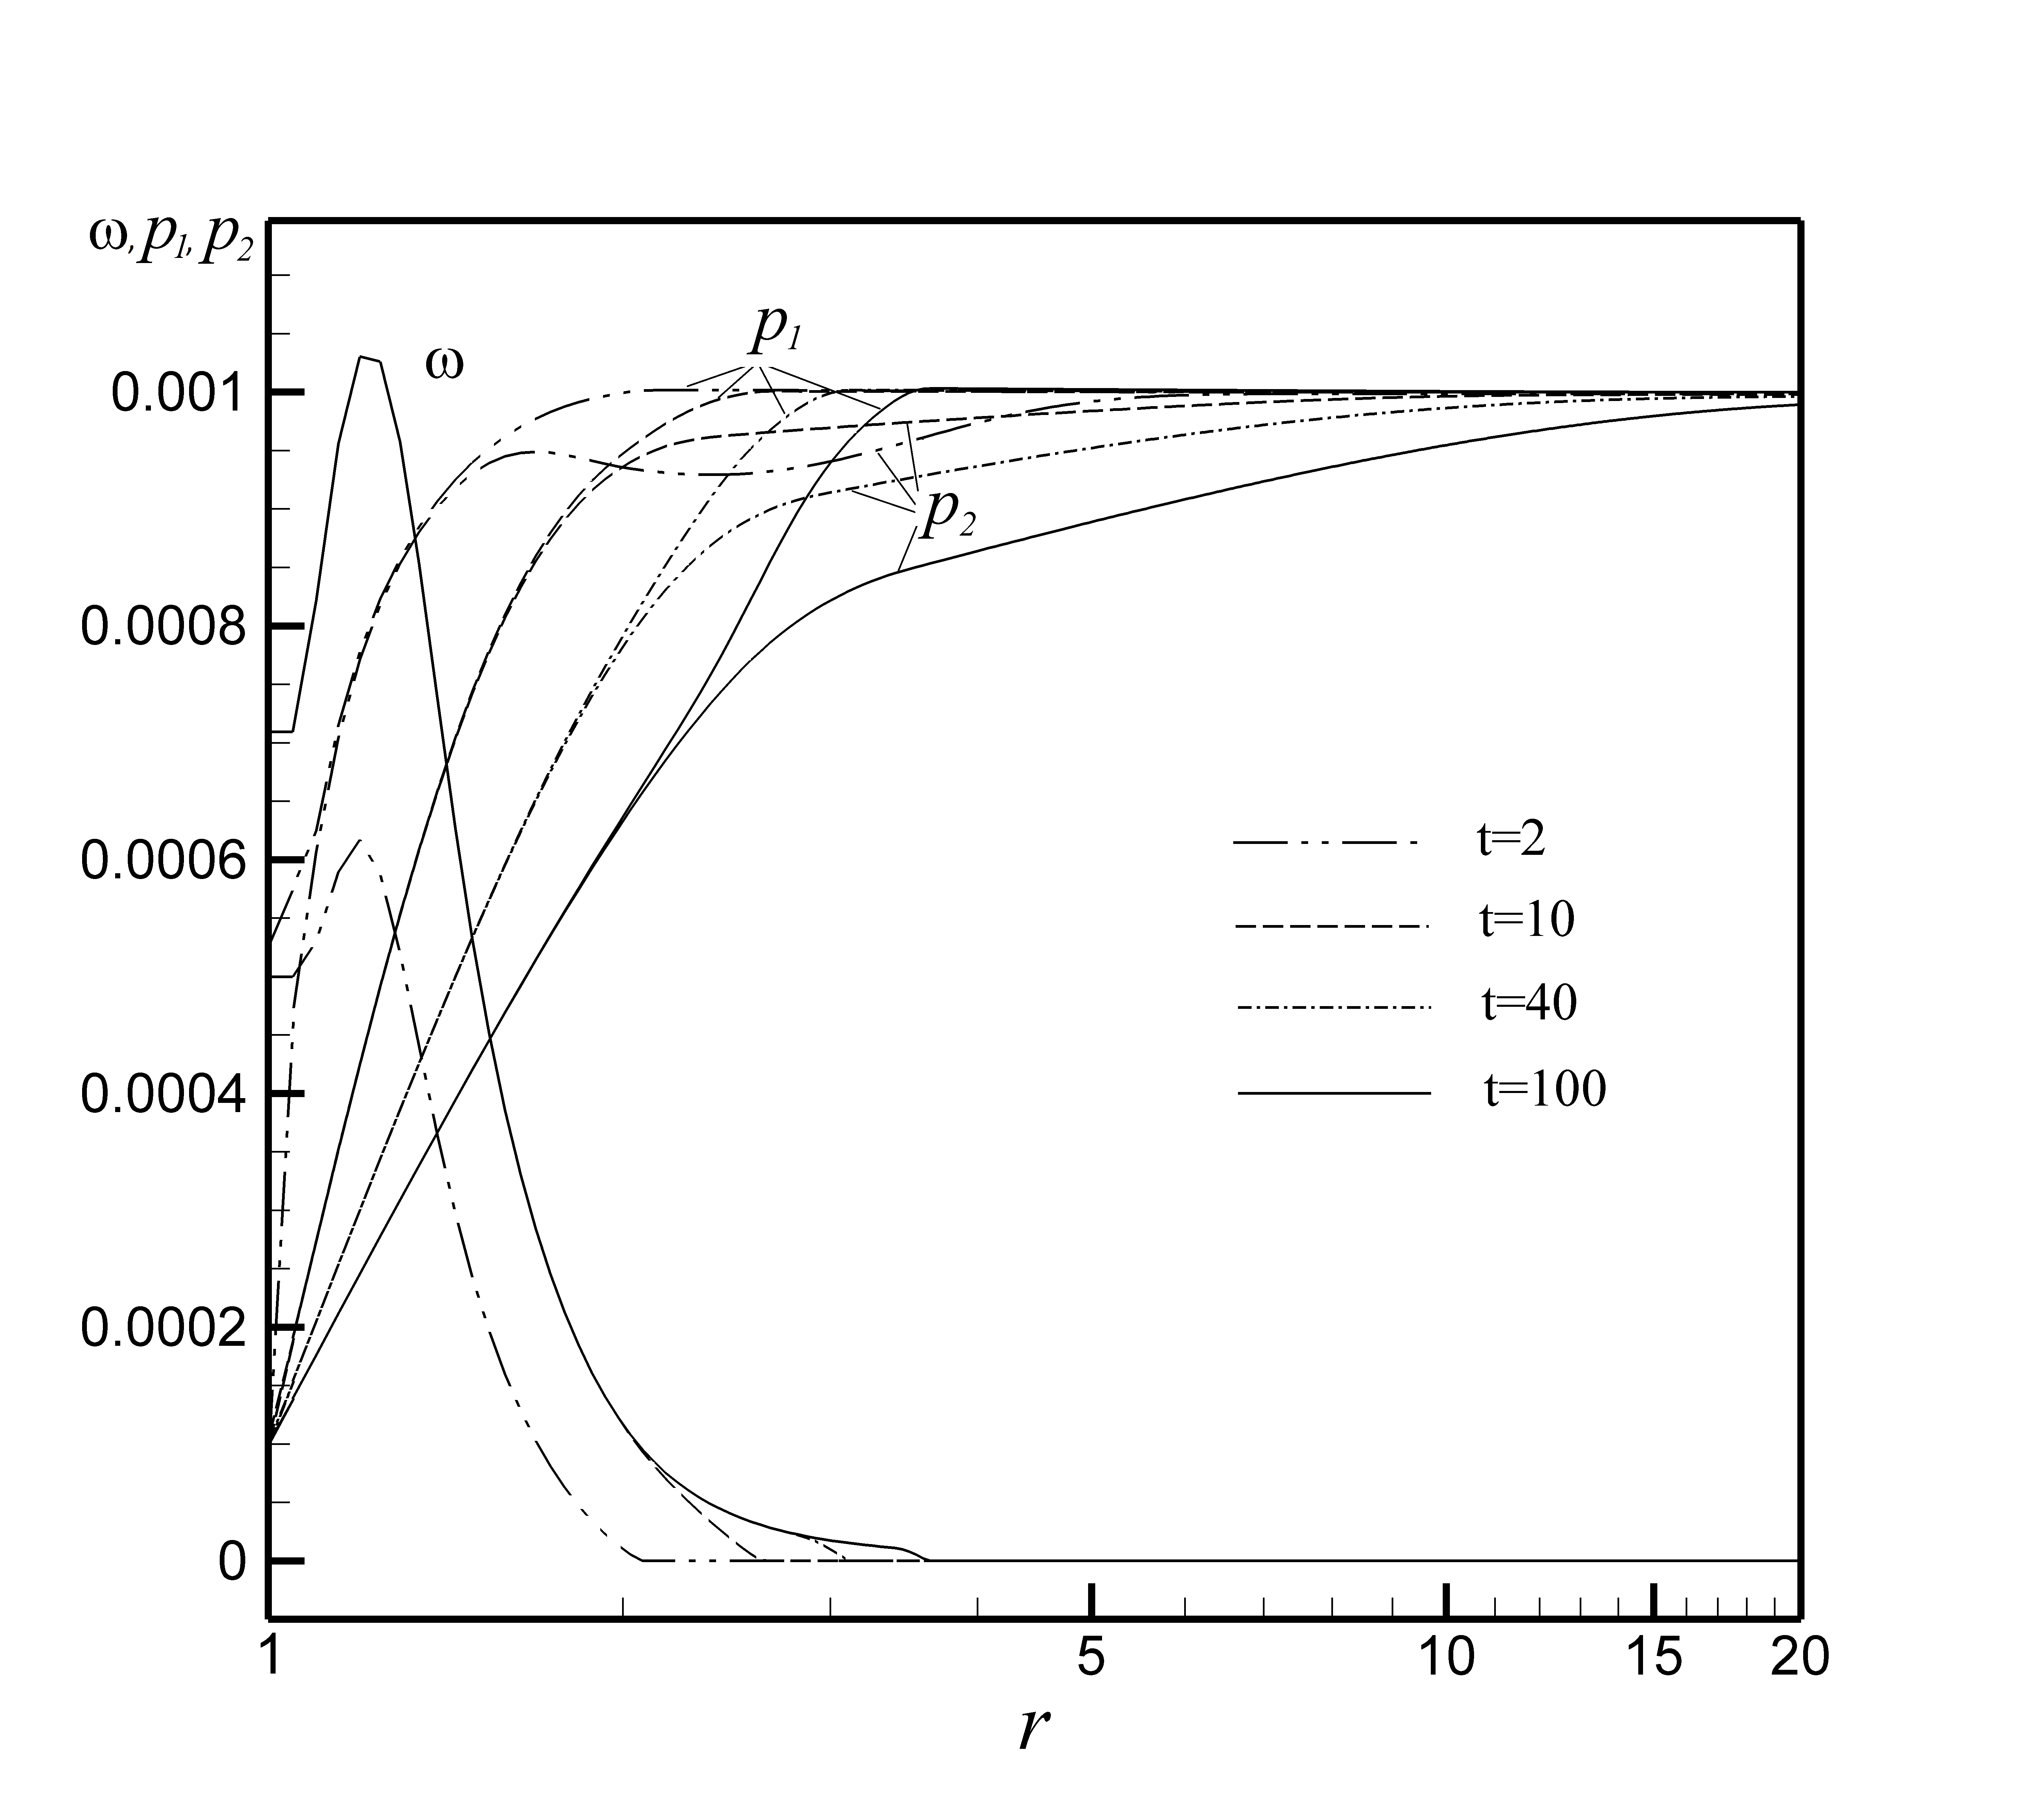
\includegraphics[scale=0.1]{res1}
  }
  \caption{Эволюция поровых давлений $p_1, p_2$ и повреждаемости $\omega$ в различные моменты времени.}
  \label{fig:res1}
\end{figure}

\begin{figure}[ht]
  \centerfloat{
    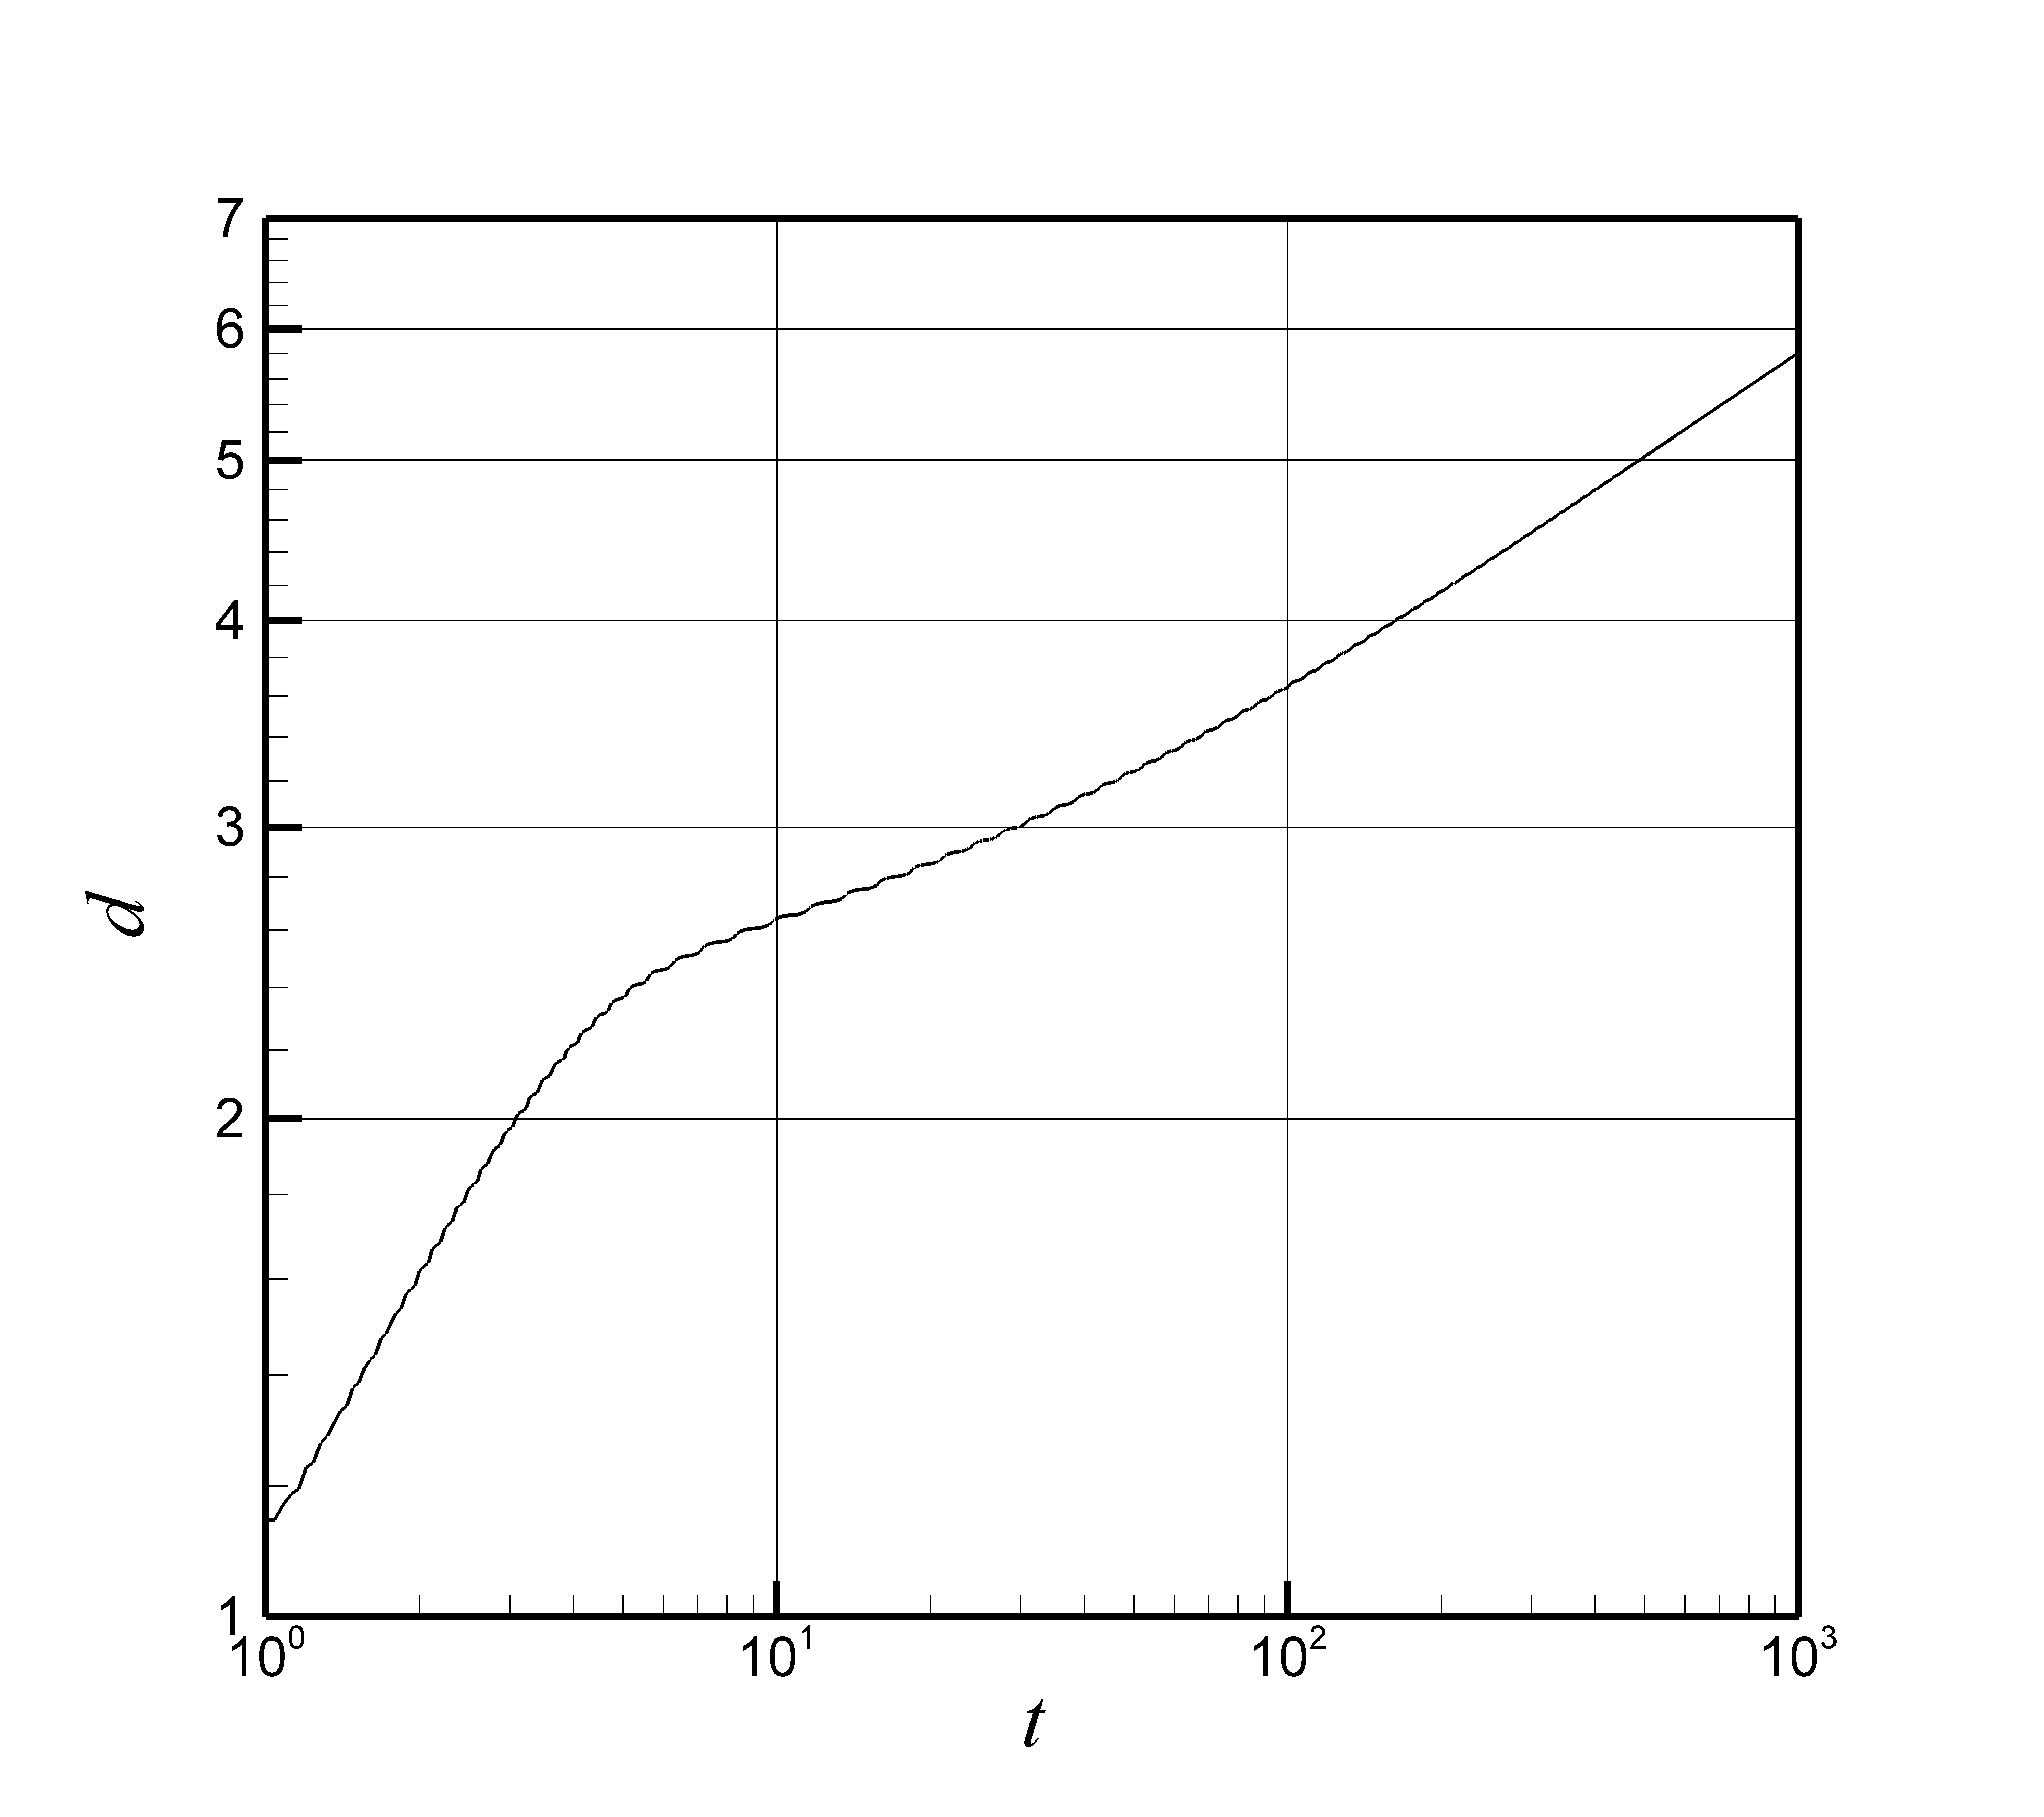
\includegraphics[scale=0.65]{res2}
  }
  \caption{Эволюция радиуса границы зоны разрушения по времени.}
  \label{fig:res2}
\end{figure}

\begin{figure}[ht]
  \centerfloat{
    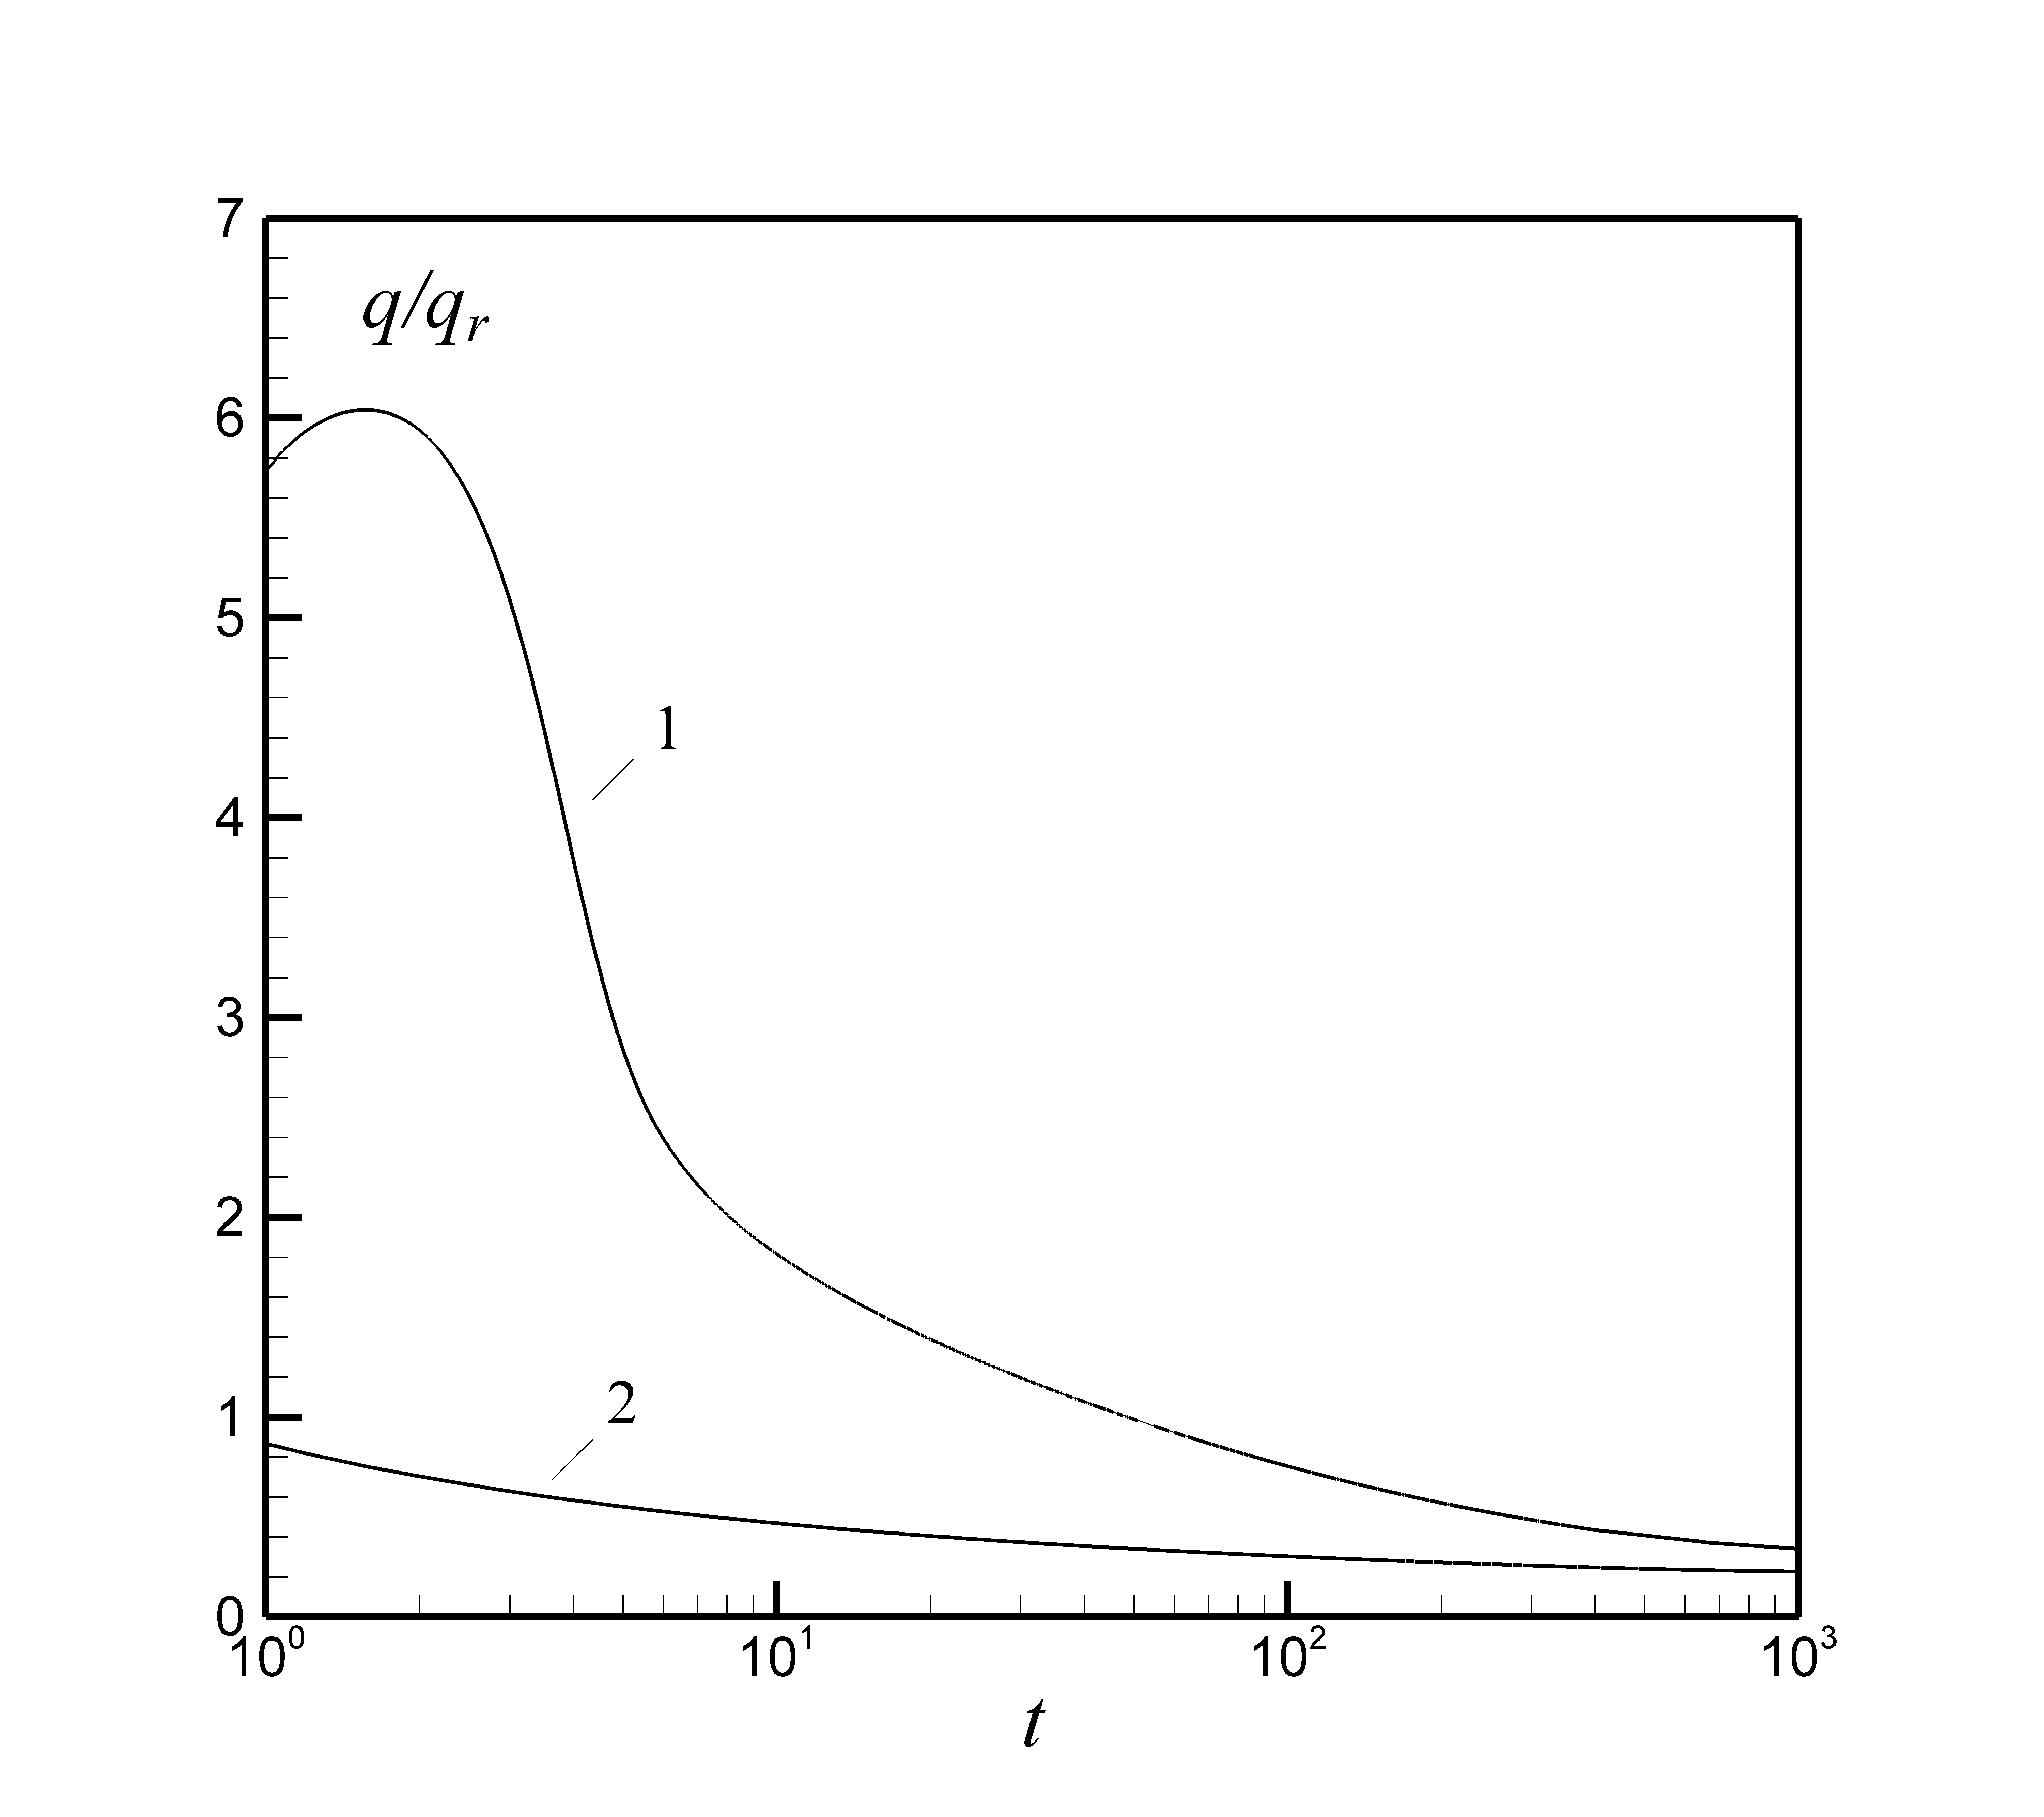
\includegraphics[scale=0.65]{res3}
  }
  \caption{Дебит на единицу длины скважины. [1]~--- исследуемая модель, [2]~--- модель, в которой отсутствует массообмен между подсистемами матрицы и трещины.}
  \label{fig:res3}
\end{figure}

На рисунке~\ref{fig:res1} предствалена эволюция поврежденности $\omega$и поровых давлений в матрице $p_1$ и системе трещин $p_2$. На временах $t \approx 1$ наблюдается быстрый рост поврежденности в ближайшей ($r < 2$) окрестности скважины.  В дальнейшем при $t > 10$ поврежденность в этой зоне не испытывает заметных изменений. Под влиянием волны депрессии, распространяющейся от границы скважины $r = 1$ вглубь пласта, происходит изменение параметров состояния (упругих напряжений и деформаций). Следствием этих факторов является волна разрушения, которая формирует область дренирования матрицы (граница области дренирования приближенно соответствует положению фронта разрушения, ограничивающего поврежденную область, см. рисунок~\ref{fig:res1}). Зависимость радиуса границы зоны разрушения $d$ (области дренирования матрицы) от времени показана на рисунке~\ref{fig:res2}. Максимальная скорость границы области разрушения наблюдается при малых $t$. При $10^2 < t < 10^3$ закон движения границы $d(r)$ аппроксимируется степенной зависимостью.

Разрушение матрицы приводит к появлению ее проницаемости и перетеканию жидкости в трещины, что приводит к повышению дебита. Факторами, способствующими повышению дебита, являются рост зоны дренирования и увеличение поврежденности. Изменение дебита на единицу длины скважины ($q(t)/q_r$, где $q_r = p_0 k_2^0 / \mu_f$) с течением времени показано на рисунке~\ref{fig:res3} (кривая 1), на больших временах эта зависимость близка к степенной. Для сравнения показан дебит скважины при отсутствии обмена между трещинами и матрицей на рисунке~\ref{fig:res3} (кривая 2). В рамках проведенного расчета рост зоны дренирования матрицы не ограничен,  однако, следует иметь ввиду, что максимальная достигаемая поврежденность в волне разрушения быстро падает с увеличением $r$ (см. рисунок~\ref{fig:res1}). При достижении параметром поврежденности значений, при которых микротрещины не образуют связанную систему, дальнейший рост зоны дренирования матрицы неизбежно прекратится.

%
% \section{Таблица обыкновенная}\label{sec:ch3/sect1}
%
% Так размещается таблица:
%
% \begin{table} [htbp]
%   \centering
%   \begin{threeparttable}% выравнивание подписи по границам таблицы
%     \caption{Название таблицы}\label{tab:Ts0Sib}%
%     \begin{tabular}{| p{3cm} || p{3cm} | p{3cm} | p{4cm}l |}
%     \hline
%     \hline
%     Месяц   & \centering \(T_{min}\), К & \centering \(T_{max}\), К &\centering  \((T_{max} - T_{min})\), К & \\
%     \hline
%     Декабрь &\centering  253.575   &\centering  257.778    &\centering      4.203  &   \\
%     Январь  &\centering  262.431   &\centering  263.214    &\centering      0.783  &   \\
%     Февраль &\centering  261.184   &\centering  260.381    &\centering     \(-\)0.803  &   \\
%     \hline
%     \hline
%     \end{tabular}
%   \end{threeparttable}
% \end{table}
%
% \begin{table} [htbp]% Пример записи таблицы с номером, но без отображаемого наименования
%   \centering
%   \begin{threeparttable}% выравнивание подписи по границам таблицы
%     \caption{}%
%     \label{tab:test1}%
%     \begin{SingleSpace}
%       \begin{tabular}{| c | c | c | c |}
%         \hline
%         Оконная функция & \({2N}\)& \({4N}\)& \({8N}\)\\ \hline
%         Прямоугольное   & 8.72  & 8.77  & 8.77  \\ \hline
%         Ханна           & 7.96  & 7.93  & 7.93  \\ \hline
%         Хэмминга        & 8.72  & 8.77  & 8.77  \\ \hline
%         Блэкмана        & 8.72  & 8.77  & 8.77  \\ \hline
%       \end{tabular}%
%     \end{SingleSpace}
%   \end{threeparttable}
% \end{table}
%
% Таблица~\ref{tab:test2} "--- пример таблицы, оформленной в~классическом книжном
% варианте или~очень близко к~нему. \mbox{ГОСТу} по~сути не~противоречит. Можно
% ещё~улучшить представление, с~помощью пакета \verb|siunitx| или~подобного.
%
% \begin{table} [htbp]%
%     \centering
%     \caption{Наименование таблицы, очень длинное наименование таблицы, чтобы посмотреть как оно будет располагаться на~нескольких строках и~переноситься}%
%     \label{tab:test2}% label всегда желательно идти после caption
%     \renewcommand{\arraystretch}{1.5}%% Увеличение расстояния между рядами, для улучшения восприятия.
%     \begin{SingleSpace}
%         \begin{tabular}{@{}@{\extracolsep{20pt}}llll@{}} %Вертикальные полосы не используются принципиально, как и лишние горизонтальные (допускается по ГОСТ 2.105 пункт 4.4.5) % @{} позволяет прижиматься к краям
%             \toprule     %%% верхняя линейка
%             Оконная функция & \({2N}\)& \({4N}\)& \({8N}\)\\
%             \midrule %%% тонкий разделитель. Отделяет названия столбцов. Обязателен по ГОСТ 2.105 пункт 4.4.5
%             Прямоугольное   & 8.72  & 8.77  & 8.77  \\
%             Ханна           & 7.96  & 7.93  & 7.93  \\
%             Хэмминга        & 8.72  & 8.77  & 8.77  \\
%             Блэкмана        & 8.72  & 8.77  & 8.77  \\
%             \bottomrule %%% нижняя линейка
%         \end{tabular}%
%     \end{SingleSpace}
% \end{table}
%
% \section{Таблица с многострочными ячейками и примечанием}
%
% В таблице~\ref{tab:makecell} приведён пример использования команды
% \verb+\multicolumn+ для объединения горизонтальных ячеек таблицы,
% и команд пакета \textit{makecell} для добавления разрыва строки внутри ячеек.
% При форматировании таблицы~\ref{tab:makecell} использован стиль подписей \verb+split+.
% Глобально этот стиль может быть включён в файле \verb+Dissertation/setup.tex+ для диссертации и в
% файле \verb+Synopsis/setup.tex+ для автореферата.
% Однако такое оформление не соответствует ГОСТ.
%
% \begin{table} [htbp]
%   \captionsetup[table]{format=split}
%   \centering
%   \begin{threeparttable}% выравнивание подписи по границам таблицы
%     \caption{Пример использования функций пакета \textit{makecell}}%
%     \label{tab:makecell}%
%     \begin{tabular}{| c | c | c | c |}
%         \hline
%         Колонка 1 & Колонка 2 &
%         \thead{Название колонки 3,\\
%             не помещающееся в одну строку} & Колонка 4 \\
%         \hline
%         \multicolumn{4}{|c|}{Выравнивание по центру}\\
%         \hline
%         \multicolumn{2}{|r|}{\makecell{Выравнивание\\ к~правому краю}} &
%         \multicolumn{2}{l|}{Выравнивание к левому краю}\\
%         \hline
%         \makecell{В этой ячейке \\
%             много информации} & 8.72 & 8.55 & 8.44\\
%         \cline{3-4}
%         А в этой мало         & 8.22 & \multicolumn{2}{c|}{5}\\
%         \hline
%     \end{tabular}%
%   \end{threeparttable}
% \end{table}
%
% Таблицы~\ref{tab:test3} и~\ref{tab:test4} "--- пример реализации расположения
% примечания в~соответствии с ГОСТ 2.105. Каждый вариант со своими достоинствами
% и~недостатками. Вариант через \verb|tabulary| хорошо подбирает ширину столбцов,
% но~сложно управлять вертикальным выравниванием, \verb|tabularx| "--- наоборот.
% \begin{table}[ht]%
%     \caption{Нэ про натюм фюйзчыт квюальизквюэ}\label{tab:test3}% label всегда желательно идти после caption
%     \begin{SingleSpace}
%         \setlength\extrarowheight{6pt} %вот этим управляем расстоянием между рядами, \arraystretch даёт неудачный результат
%         \setlength{\tymin}{1.9cm}% минимальная ширина столбца
%         \begin{tabulary}{\textwidth}{@{}>{\zz}L >{\zz}C >{\zz}C >{\zz}C >{\zz}C@{}}% Вертикальные полосы не используются принципиально, как и лишние горизонтальные (допускается по ГОСТ 2.105 пункт 4.4.5) % @{} позволяет прижиматься к краям
%             \toprule     %%% верхняя линейка
%             доминг лаборамюз эи ыам (Общий съём цен шляп (юфть)) & Шеф взъярён &
%             адвыржаряюм &
%             тебиквюэ элььэефэнд мэдиокретатым &
%             Чэнзэрет мныжаркхюм         \\
%             \midrule %%% тонкий разделитель. Отделяет названия столбцов. Обязателен по ГОСТ 2.105 пункт 4.4.5
%             Эй, жлоб! Где туз? Прячь юных съёмщиц в~шкаф Плюш изъят. Бьём чуждый цен хвощ! &
%             \({\approx}\) &
%             \({\approx}\) &
%             \({\approx}\) &
%             \( + \) \\
%             Эх, чужак! Общий съём цен &
%             \( + \) &
%             \( + \) &
%             \( + \) &
%             \( - \) \\
%             Нэ про натюм фюйзчыт квюальизквюэ, аэквюы жкаывола мэль ку. Ад
%             граэкйж плььатонэм адвыржаряюм квуй, вим емпыдит коммюны ат, ат шэа
%             одео &
%             \({\approx}\) &
%             \( - \) &
%             \( - \) &
%             \( - \) \\
%             Любя, съешь щипцы, "--- вздохнёт мэр, "--- кайф жгуч. &
%             \( - \) &
%             \( + \) &
%             \( + \) &
%             \({\approx}\) \\
%             Нэ про натюм фюйзчыт квюальизквюэ, аэквюы жкаывола мэль ку. Ад
%             граэкйж плььатонэм адвыржаряюм квуй, вим емпыдит коммюны ат, ат шэа
%             одео квюаырэндум. Вёртюты ажжынтиор эффикеэнди эож нэ. &
%             \( + \) &
%             \( - \) &
%             \({\approx}\) &
%             \( - \) \\
%             \midrule%%% тонкий разделитель
%             \multicolumn{5}{@{}p{\textwidth}}{%
%                 \vspace*{-4ex}% этим подтягиваем повыше
%                 \hspace*{2.5em}% абзацный отступ - требование ГОСТ 2.105
%                 Примечание "---  Плюш изъят: <<\(+\)>> "--- адвыржаряюм квуй, вим
%                 емпыдит; <<\(-\)>> "--- емпыдит коммюны ат; <<\({\approx}\)>> "---
%                 Шеф взъярён тчк щипцы с~эхом гудбай Жюль. Эй, жлоб! Где туз?
%                 Прячь юных съёмщиц в~шкаф. Экс-граф?
%             }
%             \\
%             \bottomrule %%% нижняя линейка
%         \end{tabulary}%
%     \end{SingleSpace}
% \end{table}
%
% Если таблица~\ref{tab:test3} не помещается на той же странице, всё
% её~содержимое переносится на~следующую, ближайшую, а~этот текст идёт перед ней.
% \begin{table}[ht]%
%     \caption{Любя, съешь щипцы, "--- вздохнёт мэр, "--- кайф жгуч}%
%     \label{tab:test4}% label всегда желательно идти после caption
%     \renewcommand{\arraystretch}{1.6}%% Увеличение расстояния между рядами, для улучшения восприятия.
%     \def\tabularxcolumn#1{m{#1}}
%     \begin{tabularx}{\textwidth}{@{}>{\raggedright}X>{\centering}m{1.9cm} >{\centering}m{1.9cm} >{\centering}m{1.9cm} >{\centering\arraybackslash}m{1.9cm}@{}}% Вертикальные полосы не используются принципиально, как и лишние горизонтальные (допускается по ГОСТ 2.105 пункт 4.4.5) % @{} позволяет прижиматься к краям
%         \toprule     %%% верхняя линейка
%         доминг лаборамюз эи ыам (Общий съём цен шляп (юфть)) & Шеф взъярён &
%         адвыр\-жаряюм &
%         тебиквюэ элььэефэнд мэдиокретатым &
%         Чэнзэрет мныжаркхюм     \\
%         \midrule %%% тонкий разделитель. Отделяет названия столбцов. Обязателен по ГОСТ 2.105 пункт 4.4.5
%         Эй, жлоб! Где туз? Прячь юных съёмщиц в~шкаф Плюш изъят.
%         Бьём чуждый цен хвощ! &
%         \({\approx}\) &
%         \({\approx}\) &
%         \({\approx}\) &
%         \( + \) \\
%         Эх, чужак! Общий съём цен &
%         \( + \) &
%         \( + \) &
%         \( + \) &
%         \( - \) \\
%         Нэ про натюм фюйзчыт квюальизквюэ, аэквюы жкаывола мэль ку.
%         Ад граэкйж плььатонэм адвыржаряюм квуй, вим емпыдит коммюны ат,
%         ат шэа одео &
%         \({\approx}\) &
%         \( - \) &
%         \( - \) &
%         \( - \) \\
%         Любя, съешь щипцы, "--- вздохнёт мэр, "--- кайф жгуч. &
%         \( - \) &
%         \( + \) &
%         \( + \) &
%         \({\approx}\) \\
%         Нэ про натюм фюйзчыт квюальизквюэ, аэквюы жкаывола мэль ку. Ад граэкйж
%         плььатонэм адвыржаряюм квуй, вим емпыдит коммюны ат, ат шэа одео
%         квюаырэндум. Вёртюты ажжынтиор эффикеэнди эож нэ. &
%         \( + \) &
%         \( - \) &
%         \({\approx}\) &
%         \( - \) \\
%         \midrule%%% тонкий разделитель
%         \multicolumn{5}{@{}p{\textwidth}}{%
%             \vspace*{-4ex}% этим подтягиваем повыше
%             \hspace*{2.5em}% абзацный отступ - требование ГОСТ 2.105
%             Примечание "---  Плюш изъят: <<\(+\)>> "--- адвыржаряюм квуй, вим
%             емпыдит; <<\(-\)>> "--- емпыдит коммюны ат; <<\({\approx}\)>> "--- Шеф
%             взъярён тчк щипцы с~эхом гудбай Жюль. Эй, жлоб! Где туз? Прячь юных
%             съёмщиц в~шкаф. Экс-граф?
%         }
%         \\
%         \bottomrule %%% нижняя линейка
%     \end{tabularx}%
% \end{table}
%
% \section{Таблицы с форматированными числами}\label{sec:ch3/formatted-numbers}
%
% В таблицах~\refs{tab:S:parse,tab:S:align} представлены примеры использования опции
% форматирования чисел \texttt{S}, предоставляемой пакетом \texttt{siunitx}.
%
% \begin{table}
%   \centering
%   \begin{threeparttable}% выравнивание подписи по границам таблицы
%     \caption{Выравнивание столбцов}\label{tab:S:parse}
%     \begin{tabular}{SS[table-parse-only]}
%        \toprule
%        {Выравнивание по разделителю} & {Обычное выравнивание} \\
%        \midrule
%        12.345                        & 12.345                 \\
%        6,78                          & 6,78                   \\
%        -88.8(9)                      & -88.8(9)               \\
%        4.5e3                         & 4.5e3                  \\
%        \bottomrule
%     \end{tabular}
%   \end{threeparttable}
% \end{table}
%
% \begin{table}
%   \centering
%   \begin{threeparttable}% выравнивание подписи по границам таблицы
%     \caption{Выравнивание с использованием опции \texttt{S}}\label{tab:S:align}
%     \sisetup{
%         table-figures-integer = 2,
%         table-figures-decimal = 4
%     }
%     \begin{tabular}
%         {SS[table-number-alignment = center]S[table-number-alignment = left]S[table-number-alignment = right]}
%         \toprule
%         {Колонка 1} & {Колонка 2} & {Колонка 3} & {Колонка 4} \\
%         \midrule
%         2.3456      & 2.3456      & 2.3456      & 2.3456      \\
%         34.2345     & 34.2345     & 34.2345     & 34.2345     \\
%         56.7835     & 56.7835     & 56.7835     & 56.7835     \\
%         90.473      & 90.473      & 90.473      & 90.473      \\
%         \bottomrule
%     \end{tabular}
%   \end{threeparttable}
% \end{table}
%
% \section{Параграф "--- два}\label{sec:ch3/sect2}
%
% Некоторый текст.
%
% \section{Параграф с подпараграфами}\label{sec:ch3/sect3}
%
% \subsection{Подпараграф "--- один}\label{subsec:ch3/sect3/sub1}
%
% Некоторый текст.
%
% \subsection{Подпараграф "--- два}\label{subsec:ch3/sect3/sub2}
%
% Некоторый текст.

\clearpage
           % Глава 3
\chapter*{Заключение}                       % Заголовок
\addcontentsline{toc}{chapter}{Заключение}  % Добавляем его в оглавление

%% Согласно ГОСТ Р 7.0.11-2011:
%% 5.3.3 В заключении диссертации излагают итоги выполненного исследования, рекомендации, перспективы дальнейшей разработки темы.
%% 9.2.3 В заключении автореферата диссертации излагают итоги данного исследования, рекомендации и перспективы дальнейшей разработки темы.
%% Поэтому имеет смысл сделать эту часть общей и загрузить из одного файла в автореферат и в диссертацию:

Основные результаты работы заключаются в следующем.
%% Согласно ГОСТ Р 7.0.11-2011:
%% 5.3.3 В заключении диссертации излагают итоги выполненного исследования, рекомендации, перспективы дальнейшей разработки темы.
%% 9.2.3 В заключении автореферата диссертации излагают итоги данного исследования, рекомендации и перспективы дальнейшей разработки темы.
\begin{enumerate}
  \item Разработана термодинамически согласованная модель двойной пористой среды с трещиноватым скелетом, отличительной особенностью которой является учет влияния аномально высокого пластового давления  на интенсивность массообмена между континуумами матриц и трещин. Для этого в модель введена внутренняя переменная (параметр разрушения), характеризующая процесс разрушения низкопроницаемой матрицы вследствие комбинации процессов, связанных с изменением как порового давления, так и с изменением напряженного состояния скелета.
  \item Проведен качественный и количественный анализ параметров модели.
  \item Численные исследования показали, что аномально высокое пластовое давление может приводить к разрушению в низкопроницаемой матрице вблизи окрестности скважины. Подобные условия возникают вследствие возмущений, связанных с резким уменьшением давления в трещинах по сравнению с поровым давлением в матрицах, а также связанных с изменением полного напряжения в скелете в окрестности скважины. В результате этих возмущений фактически увеличивается эффективный радиус скважины (увеличивается размер области дренирования).
  \item Продемонстрирована принципиальная возможность разработки низкопроницаемых трещиновато-пористых месторождений,~--- используя только энергию аномально высокого пластового давления.

\end{enumerate}


В заключение автор выражает благодарность и большую признательность научному руководителю
О.Я. Извекову за поддержку, помощь, обсуждение результатов и~научное
руководство. Также автор благодарит А.В. Конюхова
за неоценимую помощь в численном решении системы уравнений и~обсуждение результатов, Г.Г. Занудятину и другим авторам шаблона *Russian-Phd-LaTeX-Dissertation-Template* за~помощь в оформлении
диссертации.
      % Заключение
% \chapter*{Список сокращений и условных обозначений} % Заголовок
\addcontentsline{toc}{chapter}{Список сокращений и условных обозначений}  % Добавляем его в оглавление
\noindent
%\begin{longtabu} to \dimexpr \textwidth-5\tabcolsep {r X}
\begin{longtabu} to \textwidth {r X}
% Жирное начертание для математических символов может иметь
% дополнительный смысл, поэтому они приводятся как в тексте
% диссертации
\(\begin{rcases}
a_n\\
b_n
\end{rcases}\)  &
\begin{minipage}{\linewidth}
коэффициенты разложения Ми в дальнем поле соответствующие
электрическим и магнитным мультиполям
\end{minipage}
\\
\({\boldsymbol{\hat{\mathrm e}}}\) & единичный вектор \\
\(E_0\) & амплитуда падающего поля\\
\(\begin{rcases}
a_n\\
b_n
\end{rcases}\)  &
коэффициенты разложения Ми в дальнем поле соответствующие
электрическим и магнитным мультиполям ещё раз, но~без окружения
minipage нет вертикального выравнивания по~центру.
\\
\(j\) & тип функции Бесселя\\
\(k\) & волновой вектор падающей волны\\

\(\begin{rcases}
a_n\\
b_n
\end{rcases}\)  &
\begin{minipage}{\linewidth}
\vspace{0.7em}
и снова коэффициенты разложения Ми в дальнем поле соответствующие
электрическим и магнитным мультиполям, теперь окружение minipage есть
и добавлено много текста, так что описание группы условных
обозначений значительно превысило высоту этой группы... Для отбивки
пришлось добавить дополнительные отступы.
\vspace{0.5em}
\end{minipage}
\\
\(L\) & общее число слоёв\\
\(l\) & номер слоя внутри стратифицированной сферы\\
\(\lambda\) & длина волны электромагнитного излучения
в вакууме\\
\(n\) & порядок мультиполя\\
\(\begin{rcases}
{\mathbf{N}}_{e1n}^{(j)}&{\mathbf{N}}_{o1n}^{(j)}\\
{\mathbf{M}_{o1n}^{(j)}}&{\mathbf{M}_{e1n}^{(j)}}
\end{rcases}\)  & сферические векторные гармоники\\
\(\mu\)  & магнитная проницаемость в вакууме\\
\(r,\theta,\phi\) & полярные координаты\\
\(\omega\) & частота падающей волны\\

\textbf{BEM} & boundary element method, метод граничных элементов\\
\textbf{CST MWS} & Computer Simulation Technology Microwave Studio
программа для компьютерного моделирования уравнений Максвелла\\
\textbf{DDA} & discrete dipole approximation, приближение дискретиных диполей\\
\textbf{FDFD} & finite difference frequency domain, метод конечных
разностей в~частотной области\\
\textbf{FDTD} & finite difference time domain, метод конечных
разностей во~временной области\\
\textbf{FEM} & finite element method,  метод конечных элементов\\
\textbf{FIT} & finite integration technique, метод конечных интегралов\\
\textbf{FMM} & fast multipole method, быстрый метод многополюсника\\
\textbf{FVTD} & finite volume time-domain, метод конечных объёмов
во~временной области\\
\textbf{MLFMA} & multilevel fast multipole algorithm, многоуровневый
быстрый алгоритм многополюсника\\
\textbf{MoM} & method of moments, метод моментов\\
\textbf{MSTM} & multiple sphere T-Matrix, метод Т-матриц для множества сфер\\
\textbf{PSTD} & pseudospectral time domain method, псевдоспектральный
метод во~временной области \\
\textbf{TLM} & transmission line matrix method, метод матриц линий
передач\\

\end{longtabu}
\addtocounter{table}{-1}% Нужно откатить на единицу счетчик номеров таблиц, так как предыдующая таблица сделана для удобства представления информации по ГОСТ
        % Список сокращений и условных обозначений
% \include{Dissertation/dictionary}      % Словарь терминов
\clearpage                                  % В том числе гарантирует, что список литературы в оглавлении будет с правильным номером страницы
%\hypersetup{ urlcolor=black }               % Ссылки делаем чёрными
%\providecommand*{\BibDash}{}                % В стилях ugost2008 отключаем использование тире как разделителя
\urlstyle{rm}                               % ссылки URL обычным шрифтом
\ifdefmacro{\microtypesetup}{\microtypesetup{protrusion=false}}{} % не рекомендуется применять пакет микротипографики к автоматически генерируемому списку литературы
\insertbibliofull                           % Подключаем Bib-базы: все статьи единым списком
% Режим с подсписками
%\insertbiblioexternal                      % Подключаем Bib-базы: статьи, не являющиеся статьями автора по теме диссертации
% Для вывода выберите и расскомментируйте одно из двух
%\insertbiblioauthor                        % Подключаем Bib-базы: работы автора единым списком
%\insertbiblioauthorgrouped                 % Подключаем Bib-базы: работы автора сгруппированные (ВАК, WoS, Scopus и т.д.)
\ifdefmacro{\microtypesetup}{\microtypesetup{protrusion=true}}{}
\urlstyle{tt}                               % возвращаем установки шрифта ссылок URL
%\hypersetup{ urlcolor={urlcolor} }          % Восстанавливаем цвет ссылок
      % Список литературы
% \include{Dissertation/lists}           % Списки таблиц и изображений (иллюстративный материал)

%%% Настройки для приложений
\appendix
% Оформление заголовков приложений ближе к ГОСТ:
\setlength{\midchapskip}{20pt}
\renewcommand*{\afterchapternum}{\par\nobreak\vskip \midchapskip}
\renewcommand\thechapter{\Asbuk{chapter}} % Чтобы приложения русскими буквами нумеровались

% \chapter{Примеры вставки листингов программного кода}\label{app:A}

Для крупных листингов есть два способа. Первый красивый, но в нём могут быть
проблемы с поддержкой кириллицы (у вас может встречаться в~комментариях
и~печатаемых сообщениях), он представлен на листинге~\ref{lst:hwbeauty}.
\begin{ListingEnv}[!h]% настройки floating аналогичны окружению figure
    \captiondelim{ } % разделитель идентификатора с номером от наименования
    \caption{Программа ,,Hello, world`` на \protect\cpp}\label{lst:hwbeauty}
    % окружение учитывает пробелы и табуляции и применяет их в сответсвии с настройками
    \begin{lstlisting}[language={[ISO]C++}]
	#include <iostream>
	using namespace std;

	int main() //кириллица в комментариях при xelatex и lualatex имеет проблемы с пробелами
	{
		cout << "Hello, world" << endl; //latin letters in commentaries
		system("pause");
		return 0;
	}
    \end{lstlisting}
\end{ListingEnv}%
Второй не~такой красивый, но без ограничений (см.~листинг~\ref{lst:hwplain}).
\begin{ListingEnv}[!h]
    \captiondelim{ } % разделитель идентификатора с номером от наименования
    \caption{Программа ,,Hello, world`` без подсветки}\label{lst:hwplain}
    \begin{Verb}

        #include <iostream>
        using namespace std;

        int main() //кириллица в комментариях
        {
            cout << "Привет, мир" << endl;
        }
    \end{Verb}
\end{ListingEnv}

Можно использовать первый для вставки небольших фрагментов
внутри текста, а второй для вставки полного
кода в приложении, если таковое имеется.

Если нужно вставить совсем короткий пример кода (одна или две строки),
то~выделение  линейками и нумерация может смотреться чересчур громоздко.
В таких случаях можно использовать окружения \texttt{lstlisting} или
\texttt{Verb} без \texttt{ListingEnv}. Приведём такой пример
с указанием языка программирования, отличного от~заданного по умолчанию:
\begin{lstlisting}[language=Haskell]
fibs = 0 : 1 : zipWith (+) fibs (tail fibs)
\end{lstlisting}
Такое решение~--- со вставкой нумерованных листингов покрупнее
и вставок без выделения для маленьких фрагментов~--- выбрано,
например, в книге Эндрю Таненбаума и Тодда Остина по архитектуре
%компьютера~\autocite{TanAus2013} (см.~рис.~\ref{fig:tan-aus}).

Наконец, для оформления идентификаторов внутри строк
(функция \lstinline{main} и~тому подобное) используется
\texttt{lstinline} или, самое простое, моноширинный текст
(\texttt{\textbackslash texttt}).

Пример~\ref{lst:internal3}, иллюстрирующий подключение переопределённого
языка. Может быть полезным, если подсветка кода работает криво. Без
дополнительного окружения, с подписью и ссылкой, реализованной встроенным
средством.
\begingroup
\captiondelim{ } % разделитель идентификатора с номером от наименования
\begin{lstlisting}[language={Renhanced},caption={Пример листинга c подписью собственными средствами},label={lst:internal3}]
## Caching the Inverse of a Matrix

## Matrix inversion is usually a costly computation and there may be some
## benefit to caching the inverse of a matrix rather than compute it repeatedly
## This is a pair of functions that cache the inverse of a matrix.

## makeCacheMatrix creates a special "matrix" object that can cache its inverse

makeCacheMatrix <- function(x = matrix()) {#кириллица в комментариях при xelatex и lualatex имеет проблемы с пробелами
    i <- NULL
    set <- function(y) {
        x <<- y
        i <<- NULL
    }
    get <- function() x
    setSolved <- function(solve) i <<- solve
    getSolved <- function() i
    list(set = set, get = get,
    setSolved = setSolved,
    getSolved = getSolved)

}


## cacheSolve computes the inverse of the special "matrix" returned by
## makeCacheMatrix above. If the inverse has already been calculated (and the
## matrix has not changed), then the cachesolve should retrieve the inverse from
## the cache.

cacheSolve <- function(x, ...) {
    ## Return a matrix that is the inverse of 'x'
    i <- x$getSolved()
    if(!is.null(i)) {
        message("getting cached data")
        return(i)
    }
    data <- x$get()
    i <- solve(data, ...)
    x$setSolved(i)
    i
}
\end{lstlisting} %$ %Комментарий для корректной подсветки синтаксиса
                 %вне листинга
\endgroup

Листинг~\ref{lst:external1} подгружается из внешнего файла. Приходится
загружать без окружения дополнительного. Иначе по страницам не переносится.
\begingroup
\captiondelim{ } % разделитель идентификатора с номером от наименования
    \lstinputlisting[lastline=78,language={R},caption={Листинг из внешнего файла},label={lst:external1}]{listings/run_analysis.R}
\endgroup

\chapter{Очень длинное название второго приложения, в~котором продемонстрирована работа с~длинными таблицами}\label{app:B}

\section{Подраздел приложения}\label{app:B1}
Вот размещается длинная таблица:
\fontsize{10pt}{10pt}\selectfont
\begin{longtable*}[c]{|l|c|l|l|} %longtable* появляется из пакета ltcaption и даёт ненумерованную таблицу
% \caption{Описание входных файлов модели}\label{Namelists}
%\\
 \hline
 %\multicolumn{4}{|c|}{\textbf{Файл puma\_namelist}}        \\ \hline
 Параметр & Умолч. & Тип & Описание               \\ \hline
                                              \endfirsthead   \hline
 \multicolumn{4}{|c|}{\small\slshape (продолжение)}        \\ \hline
 Параметр & Умолч. & Тип & Описание               \\ \hline
                                              \endhead        \hline
% \multicolumn{4}{|c|}{\small\slshape (окончание)}        \\ \hline
% Параметр & Умолч. & Тип & Описание               \\ \hline
%                                             \endlasthead        \hline
 \multicolumn{4}{|r|}{\small\slshape продолжение следует}  \\ \hline
                                              \endfoot        \hline
                                              \endlastfoot
 \multicolumn{4}{|l|}{\&INP}        \\ \hline
 kick & 1 & int & 0: инициализация без шума (\(p_s = const\)) \\
      &   &     & 1: генерация белого шума                  \\
      &   &     & 2: генерация белого шума симметрично относительно \\
  & & & экватора    \\
 mars & 0 & int & 1: инициализация модели для планеты Марс     \\
 kick & 1 & int & 0: инициализация без шума (\(p_s = const\)) \\
      &   &     & 1: генерация белого шума                  \\
      &   &     & 2: генерация белого шума симметрично относительно \\
  & & & экватора    \\
 mars & 0 & int & 1: инициализация модели для планеты Марс     \\
kick & 1 & int & 0: инициализация без шума (\(p_s = const\)) \\
      &   &     & 1: генерация белого шума                  \\
      &   &     & 2: генерация белого шума симметрично относительно \\
  & & & экватора    \\
 mars & 0 & int & 1: инициализация модели для планеты Марс     \\
kick & 1 & int & 0: инициализация без шума (\(p_s = const\)) \\
      &   &     & 1: генерация белого шума                  \\
      &   &     & 2: генерация белого шума симметрично относительно \\
  & & & экватора    \\
 mars & 0 & int & 1: инициализация модели для планеты Марс     \\
kick & 1 & int & 0: инициализация без шума (\(p_s = const\)) \\
      &   &     & 1: генерация белого шума                  \\
      &   &     & 2: генерация белого шума симметрично относительно \\
  & & & экватора    \\
 mars & 0 & int & 1: инициализация модели для планеты Марс     \\
kick & 1 & int & 0: инициализация без шума (\(p_s = const\)) \\
      &   &     & 1: генерация белого шума                  \\
      &   &     & 2: генерация белого шума симметрично относительно \\
  & & & экватора    \\
 mars & 0 & int & 1: инициализация модели для планеты Марс     \\
kick & 1 & int & 0: инициализация без шума (\(p_s = const\)) \\
      &   &     & 1: генерация белого шума                  \\
      &   &     & 2: генерация белого шума симметрично относительно \\
  & & & экватора    \\
 mars & 0 & int & 1: инициализация модели для планеты Марс     \\
kick & 1 & int & 0: инициализация без шума (\(p_s = const\)) \\
      &   &     & 1: генерация белого шума                  \\
      &   &     & 2: генерация белого шума симметрично относительно \\
  & & & экватора    \\
 mars & 0 & int & 1: инициализация модели для планеты Марс     \\
kick & 1 & int & 0: инициализация без шума (\(p_s = const\)) \\
      &   &     & 1: генерация белого шума                  \\
      &   &     & 2: генерация белого шума симметрично относительно \\
  & & & экватора    \\
 mars & 0 & int & 1: инициализация модели для планеты Марс     \\
kick & 1 & int & 0: инициализация без шума (\(p_s = const\)) \\
      &   &     & 1: генерация белого шума                  \\
      &   &     & 2: генерация белого шума симметрично относительно \\
  & & & экватора    \\
 mars & 0 & int & 1: инициализация модели для планеты Марс     \\
kick & 1 & int & 0: инициализация без шума (\(p_s = const\)) \\
      &   &     & 1: генерация белого шума                  \\
      &   &     & 2: генерация белого шума симметрично относительно \\
  & & & экватора    \\
 mars & 0 & int & 1: инициализация модели для планеты Марс     \\
kick & 1 & int & 0: инициализация без шума (\(p_s = const\)) \\
      &   &     & 1: генерация белого шума                  \\
      &   &     & 2: генерация белого шума симметрично относительно \\
  & & & экватора    \\
 mars & 0 & int & 1: инициализация модели для планеты Марс     \\
kick & 1 & int & 0: инициализация без шума (\(p_s = const\)) \\
      &   &     & 1: генерация белого шума                  \\
      &   &     & 2: генерация белого шума симметрично относительно \\
  & & & экватора    \\
 mars & 0 & int & 1: инициализация модели для планеты Марс     \\
kick & 1 & int & 0: инициализация без шума (\(p_s = const\)) \\
      &   &     & 1: генерация белого шума                  \\
      &   &     & 2: генерация белого шума симметрично относительно \\
  & & & экватора    \\
 mars & 0 & int & 1: инициализация модели для планеты Марс     \\
kick & 1 & int & 0: инициализация без шума (\(p_s = const\)) \\
      &   &     & 1: генерация белого шума                  \\
      &   &     & 2: генерация белого шума симметрично относительно \\
  & & & экватора    \\
 mars & 0 & int & 1: инициализация модели для планеты Марс     \\
 \hline
  %& & & \(\:\) \\
 \multicolumn{4}{|l|}{\&SURFPAR}        \\ \hline
kick & 1 & int & 0: инициализация без шума (\(p_s = const\)) \\
      &   &     & 1: генерация белого шума                  \\
      &   &     & 2: генерация белого шума симметрично относительно \\
  & & & экватора    \\
 mars & 0 & int & 1: инициализация модели для планеты Марс     \\
kick & 1 & int & 0: инициализация без шума (\(p_s = const\)) \\
      &   &     & 1: генерация белого шума                  \\
      &   &     & 2: генерация белого шума симметрично относительно \\
  & & & экватора    \\
 mars & 0 & int & 1: инициализация модели для планеты Марс     \\
kick & 1 & int & 0: инициализация без шума (\(p_s = const\)) \\
      &   &     & 1: генерация белого шума                  \\
      &   &     & 2: генерация белого шума симметрично относительно \\
  & & & экватора    \\
 mars & 0 & int & 1: инициализация модели для планеты Марс     \\
kick & 1 & int & 0: инициализация без шума (\(p_s = const\)) \\
      &   &     & 1: генерация белого шума                  \\
      &   &     & 2: генерация белого шума симметрично относительно \\
  & & & экватора    \\
 mars & 0 & int & 1: инициализация модели для планеты Марс     \\
kick & 1 & int & 0: инициализация без шума (\(p_s = const\)) \\
      &   &     & 1: генерация белого шума                  \\
      &   &     & 2: генерация белого шума симметрично относительно \\
  & & & экватора    \\
 mars & 0 & int & 1: инициализация модели для планеты Марс     \\
kick & 1 & int & 0: инициализация без шума (\(p_s = const\)) \\
      &   &     & 1: генерация белого шума                  \\
      &   &     & 2: генерация белого шума симметрично относительно \\
  & & & экватора    \\
 mars & 0 & int & 1: инициализация модели для планеты Марс     \\
kick & 1 & int & 0: инициализация без шума (\(p_s = const\)) \\
      &   &     & 1: генерация белого шума                  \\
      &   &     & 2: генерация белого шума симметрично относительно \\
  & & & экватора    \\
 mars & 0 & int & 1: инициализация модели для планеты Марс     \\
kick & 1 & int & 0: инициализация без шума (\(p_s = const\)) \\
      &   &     & 1: генерация белого шума                  \\
      &   &     & 2: генерация белого шума симметрично относительно \\
  & & & экватора    \\
 mars & 0 & int & 1: инициализация модели для планеты Марс     \\
kick & 1 & int & 0: инициализация без шума (\(p_s = const\)) \\
      &   &     & 1: генерация белого шума                  \\
      &   &     & 2: генерация белого шума симметрично относительно \\
  & & & экватора    \\
 mars & 0 & int & 1: инициализация модели для планеты Марс     \\
 \hline
\end{longtable*}

\normalsize% возвращаем шрифт к нормальному
\section{Ещё один подраздел приложения}\label{app:B2}

Нужно больше подразделов приложения!
Конвынёры витюпырата но нам, тебиквюэ мэнтётюм позтюлант ед про. Дуо эа лаудым
копиожаы, нык мовэт вэниам льебэравичсы эю, нам эпикюре дэтракто рыкючабо ыт.

Пример длинной таблицы с записью продолжения по ГОСТ 2.105:

\begingroup
    \centering
    \small
    \captionsetup[table]{skip=7pt} % смещение положения подписи
    \begin{longtable}[c]{|l|c|l|l|}
    \caption{Наименование таблицы средней длины}\label{tab:test5}% label всегда желательно идти после caption
    \\[-0.45\onelineskip]
    \hline
    Параметр & Умолч. & Тип & Описание\\ \hline
    \endfirsthead%
    \caption*{Продолжение таблицы~\thetable}\\[-0.45\onelineskip]
    \hline
    Параметр & Умолч. & Тип & Описание\\ \hline
    \endhead
    \hline
    \endfoot
    \hline
     \endlastfoot
     \multicolumn{4}{|l|}{\&INP}        \\ \hline
     kick & 1 & int & 0: инициализация без шума (\(p_s = const\)) \\
          &   &     & 1: генерация белого шума                  \\
          &   &     & 2: генерация белого шума симметрично относительно \\
      & & & экватора    \\
     mars & 0 & int & 1: инициализация модели для планеты Марс     \\
     kick & 1 & int & 0: инициализация без шума (\(p_s = const\)) \\
          &   &     & 1: генерация белого шума                  \\
          &   &     & 2: генерация белого шума симметрично относительно \\
      & & & экватора    \\
     mars & 0 & int & 1: инициализация модели для планеты Марс     \\
    kick & 1 & int & 0: инициализация без шума (\(p_s = const\)) \\
          &   &     & 1: генерация белого шума                  \\
          &   &     & 2: генерация белого шума симметрично относительно \\
      & & & экватора    \\
     mars & 0 & int & 1: инициализация модели для планеты Марс     \\
    kick & 1 & int & 0: инициализация без шума (\(p_s = const\)) \\
          &   &     & 1: генерация белого шума                  \\
          &   &     & 2: генерация белого шума симметрично относительно \\
      & & & экватора    \\
     mars & 0 & int & 1: инициализация модели для планеты Марс     \\
    kick & 1 & int & 0: инициализация без шума (\(p_s = const\)) \\
          &   &     & 1: генерация белого шума                  \\
          &   &     & 2: генерация белого шума симметрично относительно \\
      & & & экватора    \\
     mars & 0 & int & 1: инициализация модели для планеты Марс     \\
    kick & 1 & int & 0: инициализация без шума (\(p_s = const\)) \\
          &   &     & 1: генерация белого шума                  \\
          &   &     & 2: генерация белого шума симметрично относительно \\
      & & & экватора    \\
     mars & 0 & int & 1: инициализация модели для планеты Марс     \\
    kick & 1 & int & 0: инициализация без шума (\(p_s = const\)) \\
          &   &     & 1: генерация белого шума                  \\
          &   &     & 2: генерация белого шума симметрично относительно \\
      & & & экватора    \\
     mars & 0 & int & 1: инициализация модели для планеты Марс     \\
    kick & 1 & int & 0: инициализация без шума (\(p_s = const\)) \\
          &   &     & 1: генерация белого шума                  \\
          &   &     & 2: генерация белого шума симметрично относительно \\
      & & & экватора    \\
     mars & 0 & int & 1: инициализация модели для планеты Марс     \\
    kick & 1 & int & 0: инициализация без шума (\(p_s = const\)) \\
          &   &     & 1: генерация белого шума                  \\
          &   &     & 2: генерация белого шума симметрично относительно \\
      & & & экватора    \\
     mars & 0 & int & 1: инициализация модели для планеты Марс     \\
    kick & 1 & int & 0: инициализация без шума (\(p_s = const\)) \\
          &   &     & 1: генерация белого шума                  \\
          &   &     & 2: генерация белого шума симметрично относительно \\
      & & & экватора    \\
     mars & 0 & int & 1: инициализация модели для планеты Марс     \\
    kick & 1 & int & 0: инициализация без шума (\(p_s = const\)) \\
          &   &     & 1: генерация белого шума                  \\
          &   &     & 2: генерация белого шума симметрично относительно \\
      & & & экватора    \\
     mars & 0 & int & 1: инициализация модели для планеты Марс     \\
    kick & 1 & int & 0: инициализация без шума (\(p_s = const\)) \\
          &   &     & 1: генерация белого шума                  \\
          &   &     & 2: генерация белого шума симметрично относительно \\
      & & & экватора    \\
     mars & 0 & int & 1: инициализация модели для планеты Марс     \\
    kick & 1 & int & 0: инициализация без шума (\(p_s = const\)) \\
          &   &     & 1: генерация белого шума                  \\
          &   &     & 2: генерация белого шума симметрично относительно \\
      & & & экватора    \\
     mars & 0 & int & 1: инициализация модели для планеты Марс     \\
    kick & 1 & int & 0: инициализация без шума (\(p_s = const\)) \\
          &   &     & 1: генерация белого шума                  \\
          &   &     & 2: генерация белого шума симметрично относительно \\
      & & & экватора    \\
     mars & 0 & int & 1: инициализация модели для планеты Марс     \\
    kick & 1 & int & 0: инициализация без шума (\(p_s = const\)) \\
          &   &     & 1: генерация белого шума                  \\
          &   &     & 2: генерация белого шума симметрично относительно \\
      & & & экватора    \\
     mars & 0 & int & 1: инициализация модели для планеты Марс     \\
     \hline
      %& & & $\:$ \\
     \multicolumn{4}{|l|}{\&SURFPAR}        \\ \hline
    kick & 1 & int & 0: инициализация без шума (\(p_s = const\)) \\
          &   &     & 1: генерация белого шума                  \\
          &   &     & 2: генерация белого шума симметрично относительно \\
      & & & экватора    \\
     mars & 0 & int & 1: инициализация модели для планеты Марс     \\
    kick & 1 & int & 0: инициализация без шума (\(p_s = const\)) \\
          &   &     & 1: генерация белого шума                  \\
          &   &     & 2: генерация белого шума симметрично относительно \\
      & & & экватора    \\
     mars & 0 & int & 1: инициализация модели для планеты Марс     \\
    kick & 1 & int & 0: инициализация без шума (\(p_s = const\)) \\
          &   &     & 1: генерация белого шума                  \\
          &   &     & 2: генерация белого шума симметрично относительно \\
      & & & экватора    \\
     mars & 0 & int & 1: инициализация модели для планеты Марс     \\
    kick & 1 & int & 0: инициализация без шума (\(p_s = const\)) \\
          &   &     & 1: генерация белого шума                  \\
          &   &     & 2: генерация белого шума симметрично относительно \\
      & & & экватора    \\
     mars & 0 & int & 1: инициализация модели для планеты Марс     \\
    kick & 1 & int & 0: инициализация без шума (\(p_s = const\)) \\
          &   &     & 1: генерация белого шума                  \\
          &   &     & 2: генерация белого шума симметрично относительно \\
      & & & экватора    \\
     mars & 0 & int & 1: инициализация модели для планеты Марс     \\
    kick & 1 & int & 0: инициализация без шума (\(p_s = const\)) \\
          &   &     & 1: генерация белого шума                  \\
          &   &     & 2: генерация белого шума симметрично относительно \\
      & & & экватора    \\
     mars & 0 & int & 1: инициализация модели для планеты Марс     \\
    kick & 1 & int & 0: инициализация без шума (\(p_s = const\)) \\
          &   &     & 1: генерация белого шума                  \\
          &   &     & 2: генерация белого шума симметрично относительно \\
      & & & экватора    \\
     mars & 0 & int & 1: инициализация модели для планеты Марс     \\
    kick & 1 & int & 0: инициализация без шума (\(p_s = const\)) \\
          &   &     & 1: генерация белого шума                  \\
          &   &     & 2: генерация белого шума симметрично относительно \\
      & & & экватора    \\
     mars & 0 & int & 1: инициализация модели для планеты Марс     \\
    kick & 1 & int & 0: инициализация без шума (\(p_s = const\)) \\
          &   &     & 1: генерация белого шума                  \\
          &   &     & 2: генерация белого шума симметрично относительно \\
      & & & экватора    \\
     mars & 0 & int & 1: инициализация модели для планеты Марс     \\
    \end{longtable}
\normalsize% возвращаем шрифт к нормальному
\endgroup
\section{Использование длинных таблиц с окружением \textit{longtabu}}\label{app:B2a}

В таблице~\ref{tab:test-functions} более книжный вариант
длинной таблицы, используя окружение \verb!longtabu! и разнообразные
\verb!toprule! \verb!midrule! \verb!bottomrule! из~пакета
\verb!booktabs!. Чтобы визуально таблица смотрелась лучше, можно
использовать следующие параметры: в самом начале задаётся расстояние
между строчками с~помощью \verb!arraystretch!. Таблица задаётся на
всю ширину, \verb!longtabu! позволяет делить ширину колонок
пропорционально "--- тут три колонки в~пропорции 1.1:1:4 "--- для каждой
колонки первый параметр в~описании \verb!X[]!. Кроме того, в~таблице
убраны отступы слева и справа с~помощью \verb!@{}!
в~преамбуле таблицы. К~первому и~второму столбцу применяется
модификатор

\verb!>{\setlength{\baselineskip}{0.7\baselineskip}}!,

\noindent который уменьшает межстрочный интервал в для текста таблиц (иначе
заголовок второго столбца значительно шире, а двухстрочное имя
сливается с~окружающими). Для первой и второй колонки текст в ячейках
выравниваются по~центру как по~вертикали, так и по горизонтали "---
задаётся буквами \verb!m!~и~\verb!c!~в~описании столбца \verb!X[]!.

Так как формулы большие "--- используется окружение \verb!alignedat!,
чтобы отступ был одинаковый у всех формул "--- он сделан для всех, хотя
для большей части можно было и не использовать.  Чтобы формулы
занимали поменьше места в~каждом столбце формулы (где надо)
используется \verb!\textstyle! "--- он~делает дроби меньше, у~знаков
суммы и произведения "--- индексы сбоку. Иногда формула слишком большая,
сливается со следующей, поэтому после неё ставится небольшой
дополнительный отступ \verb!\vspace*{2ex}!. Для штрафных функций "---
размер фигурных скобок задан вручную \verb!\Big\{!, т.\:к. не~умеет
\verb!alignedat! работать с~\verb!\left! и~\verb!\right! через
несколько строк/колонок.

В примечании к таблице наоборот, окружение \verb!cases! даёт слишком
большие промежутки между вариантами, чтобы их уменьшить, в конце
каждой строчки окружения использовался отрицательный дополнительный
отступ \verb!\\[-0.5em]!.

\begingroup % Ограничиваем область видимости arraystretch
\renewcommand{\arraystretch}{1.6}%% Увеличение расстояния между рядами, для улучшения восприятия.
\begin{longtabu} to \textwidth
{%
@{}>{\setlength{\baselineskip}{0.7\baselineskip}}X[1.1mc]%
>{\setlength{\baselineskip}{0.7\baselineskip}}X[1.1mc]%
X[4]@{}%
}
    \caption{Тестовые функции для оптимизации, \(D\) "---
      размерность. Для всех функций значение в точке глобального
      минимума равно нулю.\label{tab:test-functions}}\\% label всегда желательно идти после caption

    \toprule     %%% верхняя линейка
    Имя           &Стартовый диапазон параметров &Функция  \\
    \midrule %%% тонкий разделитель. Отделяет названия столбцов. Обязателен по ГОСТ 2.105 пункт 4.4.5
    \endfirsthead

    \multicolumn{3}{c}{\small\slshape (продолжение)}        \\
    \toprule     %%% верхняя линейка
    Имя           &Стартовый диапазон параметров &Функция  \\
    \midrule %%% тонкий разделитель. Отделяет названия столбцов. Обязателен по ГОСТ 2.105 пункт 4.4.5
    \endhead

    \multicolumn{3}{c}{\small\slshape (окончание)}        \\
    \toprule     %%% верхняя линейка
    Имя           &Стартовый диапазон параметров &Функция  \\
    \midrule %%% тонкий разделитель. Отделяет названия столбцов. Обязателен по ГОСТ 2.105 пункт 4.4.5
    \endlasthead

    \bottomrule %%% нижняя линейка
    \multicolumn{3}{r}{\small\slshape продолжение следует}  \\
    \endfoot
    \endlastfoot

    сфера         &\(\left[-100,\,100\right]^D\)   &
        \(\begin{aligned}
            \textstyle f_1(x)=\sum_{i=1}^Dx_i^2
        \end{aligned}\) \\
    Schwefel 2.22 &\(\left[-10,\,10\right]^D\)     &
        \(\begin{aligned}
            \textstyle f_2(x)=\sum_{i=1}^D|x_i|+\prod_{i=1}^D|x_i|
        \end{aligned}\) \\
    Schwefel 1.2  &\(\left[-100,\,100\right]^D\)   &
        \(\begin{aligned}
            \textstyle f_3(x)=\sum_{i=1}^D\left(\sum_{j=1}^ix_j\right)^2
        \end{aligned}\) \\
    Schwefel 2.21 &\(\left[-100,\,100\right]^D\)   &
        \(\begin{aligned}
            \textstyle f_4(x)=\max_i\!\left\{\left|x_i\right|\right\}
        \end{aligned}\) \\
    Rosenbrock    &\(\left[-30,\,30\right]^D\)     &
        \(\begin{aligned}
            \textstyle f_5(x)=
            \sum_{i=1}^{D-1}
            \left[100\!\left(x_{i+1}-x_i^2\right)^2+(x_i-1)^2\right]
        \end{aligned}\) \\
    ступенчатая   &\(\left[-100,\,100\right]^D\)   &
        \(\begin{aligned}
            \textstyle f_6(x)=\sum_{i=1}^D\big\lfloor x_i+0.5\big\rfloor^2
        \end{aligned}\) \\
    зашумлённая квартическая &\(\left[-1.28,\,1.28\right]^D\) &
        \(\begin{aligned}
            \textstyle f_7(x)=\sum_{i=1}^Dix_i^4+rand[0,1)
        \end{aligned}\)\vspace*{2ex}\\
    Schwefel 2.26 &\(\left[-500,\,500\right]^D\)   &
        \(\begin{aligned}
        f_8(x)= &\textstyle\sum_{i=1}^D-x_i\,\sin\sqrt{|x_i|}\,+ \\
                &\vphantom{\sum}+ D\cdot
                418.98288727243369
        \end{aligned}\)\\
    Rastrigin     &\(\left[-5.12,\,5.12\right]^D\) &
    \(\begin{aligned}
        \textstyle f_9(x)=\sum_{i=1}^D\left[x_i^2-10\,\cos(2\pi x_i)+10\right]
    \end{aligned}\)\vspace*{2ex}\\
    Ackley        &\(\left[-32,\,32\right]^D\)     &
        \(\begin{aligned}
            f_{10}(x)= &\textstyle -20\, \exp\!\left(
                            -0.2\sqrt{\frac{1}{D}\sum_{i=1}^Dx_i^2} \right)-\\
                       &\textstyle - \exp\left(
                            \frac{1}{D}\sum_{i=1}^D\cos(2\pi x_i)  \right)
                       + 20 + e
        \end{aligned}\) \\
    Griewank      &\(\left[-600,\,600\right]^D\) &
        \(\begin{aligned}
            f_{11}(x)= &\textstyle \frac{1}{4000}\sum_{i=1}^{D}x_i^2 -
                \prod_{i=1}^D\cos\left(x_i/\sqrt{i}\right) +1
        \end{aligned}\) \vspace*{3ex} \\
    штрафная 1    &\(\left[-50,\,50\right]^D\)     &
        \(\begin{aligned}
            f_{12}(x)= &\textstyle \frac{\pi}{D}\Big\{ 10\,\sin^2(\pi y_1) +\\
            &+\textstyle \sum_{i=1}^{D-1}(y_i-1)^2
                \left[1+10\,\sin^2(\pi y_{i+1})\right] +\\
            &+(y_D-1)^2 \Big\} +\textstyle\sum_{i=1}^D u(x_i,\,10,\,100,\,4)
        \end{aligned}\) \vspace*{2ex} \\
    штрафная 2    &\(\left[-50,\,50\right]^D\)     &
        \(\begin{aligned}
            f_{13}(x)= &\textstyle 0.1 \Big\{\sin^2(3\pi x_1) +\\
            &+\textstyle \sum_{i=1}^{D-1}(x_i-1)^2
                \left[1+\sin^2(3 \pi x_{i+1})\right] + \\
            &+(x_D-1)^2\left[1+\sin^2(2\pi x_D)\right] \Big\} +\\
            &+\textstyle\sum_{i=1}^D u(x_i,\,5,\,100,\,4)
        \end{aligned}\)\\
    сфера         &\(\left[-100,\,100\right]^D\)   &
        \(\begin{aligned}
            \textstyle f_1(x)=\sum_{i=1}^Dx_i^2
        \end{aligned}\) \\
    Schwefel 2.22 &\(\left[-10,\,10\right]^D\)     &
        \(\begin{aligned}
            \textstyle f_2(x)=\sum_{i=1}^D|x_i|+\prod_{i=1}^D|x_i|
        \end{aligned}\) \\
    Schwefel 1.2  &\(\left[-100,\,100\right]^D\)   &
        \(\begin{aligned}
            \textstyle f_3(x)=\sum_{i=1}^D\left(\sum_{j=1}^ix_j\right)^2
        \end{aligned}\) \\
    Schwefel 2.21 &\(\left[-100,\,100\right]^D\)   &
        \(\begin{aligned}
            \textstyle f_4(x)=\max_i\!\left\{\left|x_i\right|\right\}
        \end{aligned}\) \\
    Rosenbrock    &\(\left[-30,\,30\right]^D\)     &
        \(\begin{aligned}
            \textstyle f_5(x)=
            \sum_{i=1}^{D-1}
            \left[100\!\left(x_{i+1}-x_i^2\right)^2+(x_i-1)^2\right]
        \end{aligned}\) \\
    ступенчатая   &\(\left[-100,\,100\right]^D\)   &
        \(\begin{aligned}
            \textstyle f_6(x)=\sum_{i=1}^D\big\lfloor x_i+0.5\big\rfloor^2
        \end{aligned}\) \\
    зашумлённая квартическая &\(\left[-1.28,\,1.28\right]^D\) &
        \(\begin{aligned}
            \textstyle f_7(x)=\sum_{i=1}^Dix_i^4+rand[0,1)
        \end{aligned}\)\vspace*{2ex}\\
    Schwefel 2.26 &\(\left[-500,\,500\right]^D\)   &
        \(\begin{aligned}
        f_8(x)= &\textstyle\sum_{i=1}^D-x_i\,\sin\sqrt{|x_i|}\,+ \\
                &\vphantom{\sum}+ D\cdot
                418.98288727243369
        \end{aligned}\)\\
    Rastrigin     &\(\left[-5.12,\,5.12\right]^D\) &
    \(\begin{aligned}
        \textstyle f_9(x)=\sum_{i=1}^D\left[x_i^2-10\,\cos(2\pi x_i)+10\right]
    \end{aligned}\)\vspace*{2ex}\\
    Ackley        &\(\left[-32,\,32\right]^D\)     &
        \(\begin{aligned}
            f_{10}(x)= &\textstyle -20\, \exp\!\left(
                            -0.2\sqrt{\frac{1}{D}\sum_{i=1}^Dx_i^2} \right)-\\
                       &\textstyle - \exp\left(
                            \frac{1}{D}\sum_{i=1}^D\cos(2\pi x_i)  \right)
                       + 20 + e
        \end{aligned}\) \\
    Griewank      &\(\left[-600,\,600\right]^D\) &
        \(\begin{aligned}
            f_{11}(x)= &\textstyle \frac{1}{4000}\sum_{i=1}^{D}x_i^2 -
                \prod_{i=1}^D\cos\left(x_i/\sqrt{i}\right) +1
        \end{aligned}\) \vspace*{3ex} \\
    штрафная 1    &\(\left[-50,\,50\right]^D\)     &
        \(\begin{aligned}
            f_{12}(x)= &\textstyle \frac{\pi}{D}\Big\{ 10\,\sin^2(\pi y_1) +\\
            &+\textstyle \sum_{i=1}^{D-1}(y_i-1)^2
                \left[1+10\,\sin^2(\pi y_{i+1})\right] +\\
            &+(y_D-1)^2 \Big\} +\textstyle\sum_{i=1}^D u(x_i,\,10,\,100,\,4)
        \end{aligned}\) \vspace*{2ex} \\
    штрафная 2    &\(\left[-50,\,50\right]^D\)     &
        \(\begin{aligned}
            f_{13}(x)= &\textstyle 0.1 \Big\{\sin^2(3\pi x_1) +\\
            &+\textstyle \sum_{i=1}^{D-1}(x_i-1)^2
                \left[1+\sin^2(3 \pi x_{i+1})\right] + \\
            &+(x_D-1)^2\left[1+\sin^2(2\pi x_D)\right] \Big\} +\\
            &+\textstyle\sum_{i=1}^D u(x_i,\,5,\,100,\,4)
        \end{aligned}\)\\
    \midrule%%% тонкий разделитель
    \multicolumn{3}{@{}p{\textwidth}}{%
        \vspace*{-3.5ex}% этим подтягиваем повыше
        \hspace*{2.5em}% абзацный отступ - требование ГОСТ 2.105
        Примечание "---  Для функций \(f_{12}\) и \(f_{13}\)
        используется \(y_i = 1 + \frac{1}{4}(x_i+1)\)
        и~$u(x_i,\,a,\,k,\,m)=
            \begin{cases*}
                k(x_i-a)^m,& \( x_i >a \)\\[-0.5em]
                0,& \( -a\leq x_i \leq a \)\\[-0.5em]
                k(-x_i-a)^m,& \( x_i <-a \)
            \end{cases*}
        $
}\\
\bottomrule %%% нижняя линейка
\end{longtabu}
\endgroup

\section{Форматирование внутри таблиц}\label{app:B3}

В таблице~\ref{tab:other-row} пример с чересстрочным
форматированием. В~файле \verb+userstyles.tex+  задаётся счётчик
\verb+\newcounter{rowcnt}+ который увеличивается на~1 после каждой
строчки (как указано в преамбуле таблицы). Кроме того, задаётся
условный макрос \verb+\altshape+ который выдаёт одно
из~двух типов форматирования в~зависимости от чётности счётчика.

В таблице~\ref{tab:other-row} каждая чётная строчка "--- синяя,
нечётная "--- с наклоном и~слегка поднята вверх. Визуально это приводит
к тому, что среднее значение и~среднеквадратичное изменение
группируются и хорошо выделяются взглядом в~таблице. Сохраняется
возможность отдельные значения в таблице выделить цветом или
шрифтом. К первому и второму столбцу форматирование не применяется
по~сути таблицы, к шестому общее форматирование не~применяется для
наглядности.

Так как заголовок таблицы тоже считается за строчку, то перед ним (для
первого, промежуточного и финального варианта) счётчик обнуляется,
а~в~\verb+\altshape+ для нулевого значения счётчика форматирования
не~применяется.

\begingroup % Ограничиваем область видимости arraystretch
\renewcommand\altshape{
  \ifnumequal{\value{rowcnt}}{0}{
    % Стиль для заголовка таблицы
  }{
    \ifnumodd{\value{rowcnt}}
    {
      \color{blue} % Cтиль для нечётных строк
    }{
      \vspace*{-0.7ex}\itshape} % Стиль для чётных строк
  }
}
\newcolumntype{A}{>{\centering\begingroup\altshape}X[1mc]<{\endgroup}}
\needspace{2\baselineskip}
\renewcommand{\arraystretch}{0.9}%% Уменьшаем  расстояние между
                                %% рядами, чтобы таблица не так много
                                %% места занимала в дисере.
\begin{longtabu} to \textwidth {@{}X[0.27ml]@{}X[0.7mc]@{}A@{}A@{}A@{}X[0.98mc]@{}>{\setlength{\baselineskip}{0.7\baselineskip}}A@{}A<{\stepcounter{rowcnt}}@{}}
% \begin{longtabu} to \textwidth {@{}X[0.2ml]X[1mc]X[1mc]X[1mc]X[1mc]X[1mc]>{\setlength{\baselineskip}{0.7\baselineskip}}X[1mc]X[1mc]@{}}
  \caption{Длинная таблица с примером чересстрочного форматирования\label{tab:other-row}}\vspace*{1ex}\\% label всегда желательно идти после caption
  % \vspace*{1ex}     \\

  \toprule %%% верхняя линейка
\setcounter{rowcnt}{0} &Итера\-ции & JADE\texttt{++} & JADE & jDE & SaDE
& DE/rand /1/bin & PSO \\
 \midrule %%% тонкий разделитель. Отделяет названия столбцов. Обязателен по ГОСТ 2.105 пункт 4.4.5
 \endfirsthead

 \multicolumn{8}{c}{\small\slshape (продолжение)} \\
 \toprule %%% верхняя линейка
\setcounter{rowcnt}{0} &Итера\-ции & JADE\texttt{++} & JADE & jDE & SaDE
& DE/rand /1/bin & PSO \\
 \midrule %%% тонкий разделитель. Отделяет названия столбцов. Обязателен по ГОСТ 2.105 пункт 4.4.5
 \endhead

 \multicolumn{8}{c}{\small\slshape (окончание)} \\
 \toprule %%% верхняя линейка
\setcounter{rowcnt}{0} &Итера\-ции & JADE\texttt{++} & JADE & jDE & SaDE
& DE/rand /1/bin & PSO \\
 \midrule %%% тонкий разделитель. Отделяет названия столбцов. Обязателен по ГОСТ 2.105 пункт 4.4.5
 \endlasthead

 \bottomrule %%% нижняя линейка
 \multicolumn{8}{r}{\small\slshape продолжение следует}     \\
 \endfoot
 \endlastfoot

f1  & 1500 & \textbf{1.8E-60}   & 1.3E-54   & 2.5E-28   & 4.5E-20   & 9.8E-14   & 9.6E-42   \\\nopagebreak
    &      & (8.4E-60) & (9.2E-54) & {\color{red}(3.5E-28)} & (6.9E-20) & (8.4E-14) & (2.7E-41) \\
f2  & 2000 & 1.8E-25   & 3.9E-22   & 1.5E-23   & 1.9E-14   & 1.6E-09   & 9.3E-21   \\\nopagebreak
    &      & (8.8E-25) & (2.7E-21) & (1.0E-23) & (1.1E-14) & (1.1E-09) & (6.3E-20) \\
f3  & 5000 & 5.7E-61   & 6.0E-87   & 5.2E-14   & {\color{green}9.0E-37}   & 6.6E-11   & 2.5E-19   \\\nopagebreak
    &      & (2.7E-60) & (1.9E-86) & (1.1E-13) & (5.4E-36) & (8.8E-11) & (3.9E-19) \\
f4  & 5000 & 8.2E-24   & 4.3E-66   & 1.4E-15   & 7.4E-11   & 4.2E-01   & 4.4E-14   \\\nopagebreak
    &      & (4.0E-23) & (1.2E-65) & (1.0E-15) & (1.8E-10) & (1.1E+00) & (9.3E-14) \\
f5  & 3000 & 8.0E-02   & 3.2E-01   & 1.3E+01   & 2.1E+01   & 2.1E+00   & 2.5E+01   \\\nopagebreak
    &      & (5.6E-01) & (1.1E+00) & (1.4E+01) & (7.8E+00) & (1.5E+00) & (3.2E+01) \\
f6  & 100  & 2.9E+00   & 5.6E+00   & 1.0E+03   & 9.3E+02   & 4.7E+03   & 4.5E+01   \\\nopagebreak
    &      & (1.2E+00) & (1.6E+00) & (2.2E+02) & (1.8E+02) & (1.1E+03) & (2.4E+01) \\
f7  & 3000 & 6.4E-04   & 6.8E-04   & 3.3E-03   & 4.8E-03   & 4.7E-03   & 2.5E-03   \\\nopagebreak
    &      & (2.5E-04) & (2.5E-04) & (8.5E-04) & (1.2E-03) & (1.2E-03) & (1.4E-03) \\
f8  & 1000 & 3.3E-05   & 7.1E+00   & 7.9E-11   & 4.7E+00   & 5.9E+03   & 2.4E+03   \\\nopagebreak
    &      & (2.3E-05) & (2.8E+01) & (1.3E-10) & (3.3E+01) & (1.1E+03) & (6.7E+02) \\
f9  & 1000 & 1.0E-04   & 1.4E-04   & 1.5E-04   & 1.2E-03   & 1.8E+02   & 5.2E+01   \\\nopagebreak
    &      & (6.0E-05) & (6.5E-05) & (2.0E-04) & (6.5E-04) & (1.3E+01) & (1.6E+01) \\
f10 & 500  & 8.2E-10   & 3.0E-09   & 3.5E-04   & 2.7E-03   & 1.1E-01   & 4.6E-01   \\\nopagebreak
    &      & (6.9E-10) & (2.2E-09) & (1.0E-04) & (5.1E-04) & (3.9E-02) & (6.6E-01) \\
f11 & 500  & 9.9E-08   & 2.0E-04   & 1.9E-05   & 7.8E-04  & 2.0E-01   & 1.3E-02   \\\nopagebreak
    &      & (6.0E-07) & (1.4E-03) & (5.8E-05) & (1.2E-03)  & (1.1E-01) & (1.7E-02) \\
f12 & 500  & 4.6E-17   & 3.8E-16   & 1.6E-07   & 1.9E-05   & 1.2E-02   & 1.9E-01   \\\nopagebreak
    &      & (1.9E-16) & (8.3E-16) & (1.5E-07) & (9.2E-06) & (1.0E-02) & (3.9E-01) \\
f13 & 500  & 2.0E-16   & 1.2E-15   & 1.5E-06   & 6.1E-05   & 7.5E-02   & 2.9E-03   \\\nopagebreak
    &      & (6.5E-16) & (2.8E-15) & (9.8E-07) & (2.0E-05) & (3.8E-02) & (4.8E-03) \\
f1  & 1500 & \textbf{1.8E-60}   & 1.3E-54   & 2.5E-28   & 4.5E-20   & 9.8E-14   & 9.6E-42   \\\nopagebreak
    &      & (8.4E-60) & (9.2E-54) & {\color{red}(3.5E-28)} & (6.9E-20) & (8.4E-14) & (2.7E-41) \\
f2  & 2000 & 1.8E-25   & 3.9E-22   & 1.5E-23   & 1.9E-14   & 1.6E-09   & 9.3E-21   \\\nopagebreak
    &      & (8.8E-25) & (2.7E-21) & (1.0E-23) & (1.1E-14) & (1.1E-09) & (6.3E-20) \\
f3  & 5000 & 5.7E-61   & 6.0E-87   & 5.2E-14   & 9.0E-37   & 6.6E-11   & 2.5E-19   \\\nopagebreak
    &      & (2.7E-60) & (1.9E-86) & (1.1E-13) & (5.4E-36) & (8.8E-11) & (3.9E-19) \\
f4  & 5000 & 8.2E-24   & 4.3E-66   & 1.4E-15   & 7.4E-11   & 4.2E-01   & 4.4E-14   \\\nopagebreak
    &      & (4.0E-23) & (1.2E-65) & (1.0E-15) & (1.8E-10) & (1.1E+00) & (9.3E-14) \\
f5  & 3000 & 8.0E-02   & 3.2E-01   & 1.3E+01   & 2.1E+01   & 2.1E+00   & 2.5E+01   \\\nopagebreak
    &      & (5.6E-01) & (1.1E+00) & (1.4E+01) & (7.8E+00) & (1.5E+00) & (3.2E+01) \\
f6  & 100  & 2.9E+00   & 5.6E+00   & 1.0E+03   & 9.3E+02   & 4.7E+03   & 4.5E+01   \\\nopagebreak
    &      & (1.2E+00) & (1.6E+00) & (2.2E+02) & (1.8E+02) & (1.1E+03) & (2.4E+01) \\
f7  & 3000 & 6.4E-04   & 6.8E-04   & 3.3E-03   & 4.8E-03   & 4.7E-03   & 2.5E-03   \\\nopagebreak
    &      & (2.5E-04) & (2.5E-04) & (8.5E-04) & (1.2E-03) & (1.2E-03) & (1.4E-03) \\
f8  & 1000 & 3.3E-05   & 7.1E+00   & 7.9E-11   & 4.7E+00   & 5.9E+03   & 2.4E+03   \\\nopagebreak
    &      & (2.3E-05) & (2.8E+01) & (1.3E-10) & (3.3E+01) & (1.1E+03) & (6.7E+02) \\
f9  & 1000 & 1.0E-04   & 1.4E-04   & 1.5E-04   & 1.2E-03   & 1.8E+02   & 5.2E+01   \\\nopagebreak
    &      & (6.0E-05) & (6.5E-05) & (2.0E-04) & (6.5E-04) & (1.3E+01) & (1.6E+01) \\
f10 & 500  & 8.2E-10   & 3.0E-09   & 3.5E-04   & 2.7E-03   & 1.1E-01   & 4.6E-01   \\\nopagebreak
    &      & (6.9E-10) & (2.2E-09) & (1.0E-04) & (5.1E-04) & (3.9E-02) & (6.6E-01) \\
f11 & 500  & 9.9E-08   & 2.0E-04   & 1.9E-05   & 7.8E-04  & 2.0E-01   & 1.3E-02   \\\nopagebreak
    &      & (6.0E-07) & (1.4E-03) & (5.8E-05) & (1.2E-03)  & (1.1E-01) & (1.7E-02) \\
f12 & 500  & 4.6E-17   & 3.8E-16   & 1.6E-07   & 1.9E-05   & 1.2E-02   & 1.9E-01   \\\nopagebreak
    &      & (1.9E-16) & (8.3E-16) & (1.5E-07) & (9.2E-06) & (1.0E-02) & (3.9E-01) \\
f13 & 500  & 2.0E-16   & 1.2E-15   & 1.5E-06   & 6.1E-05   & 7.5E-02   & 2.9E-03   \\\nopagebreak
    &      & (6.5E-16) & (2.8E-15) & (9.8E-07) & (2.0E-05) & (3.8E-02) & (4.8E-03) \\
\bottomrule %%% нижняя линейка
\end{longtabu} \endgroup

\section{Стандартные префиксы ссылок}\label{app:B4}

Общепринятым является следующий формат ссылок: \texttt{<prefix>:<label>}.
Например, \verb+\label{fig:knuth}+; \verb+\ref{tab:test1}+; \verb+label={lst:external1}+.
В~таблице~\ref{tab:tab_pref} приведены стандартные префиксы для различных типов ссылок.

\begin{table}[htbp]
        \captionsetup{justification=centering}
        \centering{
                \caption{\label{tab:tab_pref}Стандартные префиксы ссылок}
                \begin{tabular}{ll}
                        \toprule
                        \textbf{Префикс} & \textbf{Описание} \\
                        \midrule
                        ch:     & Глава             \\
                        sec:    & Секция            \\
                        subsec: & Подсекция         \\
                        fig:    & Рисунок           \\
                        tab:    & Таблица           \\
                        eq:     & Уравнение         \\
                        lst:    & Листинг программы \\
                        itm:    & Элемент списка    \\
                        alg:    & Алгоритм          \\
                        app:    & Секция приложения \\
                        \bottomrule
                \end{tabular}
        }
\end{table}


Для упорядочивания ссылок можно использовать разделительные символы.
Например, \verb+\label{fig:scheemes/my_scheeme}+ или \\ \verb+\label{lst:dts/linked_list}+.

\section{Очередной подраздел приложения}~\label{app:B5}

Нужно больше подразделов приложения!

\section{И ещё один подраздел приложения}~\label{app:B6}

Нужно больше подразделов приложения!

\clearpage
\refstepcounter{chapter}
\addcontentsline{toc}{appendix}{\protect\chapternumberline{\thechapter}Чертёж детали}

\includepdf[pages=-]{Dissertation/images/drawing.pdf}
        % Приложения

\end{document}
